
\documentclass[12pt]{ucthesis}

%%%%%%%%%%%%%%%%%
% some packages %
%%%%%%%%%%%%%%%%%
\usepackage{apjabbrev} % journal abbreviation definitions used by apj.bst
\usepackage{amssymb}    
\usepackage{graphicx}
\usepackage{color}
\usepackage{times}     % my preference: otherwise uses computer modern fonts
\usepackage{natbib}
\bibpunct{(}{)}{;}{a}{}{,}         % formatting for natbib package
\usepackage[rightcaption]{sidecap} % defines the SCfigure environment

%%%%%%%%%%%%%%%%%%%%
% fancyhdr package %
%%%%%%%%%%%%%%%%%%%%
\usepackage{fancyhdr} 
\pagestyle{fancy}

% with this we ensure that the chapter and section headings are in lowercase.
\renewcommand{\chaptermark}[1]{\markboth{#1}{}}
\renewcommand{\sectionmark}[1]{\markright{\thesection\ #1}}
\fancyhf{} % delete current setting for header and footer
\fancyhead[LE,RO]{\bfseries\thepage}
\fancyhead[LO]{\bfseries\rightmark}
\fancyhead[RE]{\bfseries\leftmark}
\renewcommand{\headrulewidth}{0.5pt}
\renewcommand{\footrulewidth}{0pt}
\addtolength{\headheight}{0.5pt} % make space for the rule
\fancypagestyle{plain}{%
\fancyhead[RO]{\bfseries\thepage}
\fancyhead[LO]{} % get rid of headers on plain pages
\addtolength{\headheight}{0.5pt}
\renewcommand{\headrulewidth}{0pt} % and the line
}

%%%%%%%%%%%%%%%%%%%%
% ccaption package %
%%%%%%%%%%%%%%%%%%%%
\usepackage{ccaption}
\captionnamefont{\footnotesize\bfseries} % e.g., `Figure 1.1.'
\captiontitlefont{\footnotesize}         % the caption itself
\captiondelim{. }                      % e.g., `Figure 1.1. ' vs `Figure 1.1: ' 

%%%%%%%%%%%%%%%%%%%%
% hyperref package %
%%%%%%%%%%%%%%%%%%%%
\usepackage{hyperref}
\urlstyle{same}
\hypersetup{
    pdftitle={PhD Thesis: High-Redshift Type Ia Supernova Rates},
    pdfauthor={Kyle Harris Barbary},
    colorlinks=true, % false = boxed links; true = colored links
    linkcolor=black, % color of internal links
    citecolor=black, % color of links to bibliography
    urlcolor=black,  % color of external links
    breaklinks=true  %allow breaking author names across lines to avoid line 
                     %overflow
}

%%%%%%%%%%%
%COMMANDS %
%%%%%%%%%%%
\def\ssp{\def\baselinestretch{1}\large\normalsize}\ssp %hack for single-spacing
\def\nodata{\dots}
\def\phn{\phantom{0}}
\newcommand{\NOTE}[1]{{\color{red}[{\it #1}]}} %for notes in draft
\hyphenation{MAG-AUTO}


%%%%%%%%%%%%%%%%%%%
%   Frontmatter   %
%%%%%%%%%%%%%%%%%%%
\begin{document}
\title{High-Redshift Type Ia Supernova Rates in Galaxy 
Cluster and Field Environments}
\author{Kyle Harris Barbary}

\degreeyear{2011}
\degreesemester{Spring}
\degree{Doctor of Philosophy}

\numberofmembers{3}
\numberofchairs{1}
\chair{Professor Saul Perlmutter}
\othermembers{Professor William Holzapfel\\
  Professor Joshua Bloom}

\field{Physics}
\campus{Berkeley}

\maketitle
%\approvalpage
\copyrightpage

\begin{abstract}
\ssp

This thesis presents Type~Ia supernova (SN~Ia) rates from
the \emph{Hubble Space Telescope (HST)} Cluster Supernova Survey, a program
designed to efficiently detect and observe high-redshift supernovae by
targeting massive galaxy clusters at redshifts $0.9 < z <1.46$. Among
other uses, measurements of the rate at which SNe~Ia occur can be used
to help constrain the SN~Ia ``progenitor scenario.''  The progenitor
scenario, the process that leads to a SN~Ia, is a particularly poorly
understood aspect of these events. Fortunately, the progenitor is
directly linked to the delay time between star formation and supernova
explosion. Supernova rates can be used to measure the distribution of
these delay times and thus yield information about the elusive
progenitors.

Galaxy clusters, with their simpler star formation histories, offer an
ideal environment for measuring the delay time distribution. In this
thesis the SN~Ia rate in clusters is calculated based on $8 \pm 1$
cluster SNe~Ia discovered in the \emph{HST} Cluster Supernova
Survey. This is the first cluster SN~Ia rate measurement with detected
$z>0.9$ SNe. The SN~Ia rate is found to be $0.50^{+0.23}_{-0.19}$
(stat) $^{+0.10}_{-0.09}$ (sys) $h_{70}^2$ SNuB (SNuB $\equiv
10^{-12}$ SNe~$L_{\odot,B}^{-1}$~yr$^{-1}$), or in units of stellar
mass, $0.36^{+0.16}_{-0.13}$ (stat) $^{+0.07}_{-0.06}$ (sys)
$h_{70}^2$ SNuM (SNuM $\equiv 10^{-12}$
SNe~$M_\odot^{-1}$~yr$^{-1}$). This represents a factor of $\approx
5 \pm 2$ increase over measurements of the cluster rate at $z<0.2$ and
is the first significant detection of a changing cluster SN~Ia rate
with redshift. Parameterizing the late-time SN~Ia delay time
distribution with a power law ($\Psi(t) \propto t^s$), this
measurement in combination with lower-redshift cluster SN~Ia rates
constrains $s = -1.41^{+0.47}_{-0.40}$, under the approximation of a
single-burst cluster formation redshift of $z_f = 3$.  This is
generally consistent with expectations for the ``double degenerate''
progenitor scenario and inconsistent with some models for the ``single
degenerate'' progenitor scenario predicting a steeper delay time distribution at
large delay times.  To check for environmental dependence and the
influence of younger stellar populations the rate is also calculated
specifically in cluster red-sequence galaxies and in morphologically
early-type galaxies, with results similar to the full cluster
rate. Finally, the upper limit of one host-less cluster SN~Ia detected
in the survey implies that the fraction of stars in the intra-cluster
medium is less than 0.47 ($95\%$ confidence), consistent with
measurements at lower redshifts.

The volumetric SN~Ia rate can also be used to constrain the SN~Ia
delay time distribution. However, there have been discrepancies in
recent analyses of both the high-redshift rate and its implications
for the delay time distribution.  Here, the volumetric SN~Ia rate out
to $z \sim 1.6$ is measured, based on $\sim$12 SNe~Ia in the
foregrounds and backgrounds of the clusters targeted in the survey.
The rate is measured in four broad redshift bins. The results are
consistent with previous measurements at $z \gtrsim 1$ and strengthen
the case for a SN~Ia rate that is $\gtrsim$$0.6 \times 10^{-4}
h_{70}^{3}$~yr$^{-1}$~Mpc$^{-3}$ at $z \sim 1$ and flattening out at
higher redshift. Assumptions about host-galaxy dust extinction used in
different high-redshift rate measurements are examined. Different
assumptions may account for some of the difference in published
results for the $z \sim 1$ rate.

\end{abstract}

\begin{frontmatter}

\begin{dedication}
\null\vfil
{\large\raggedleft\it
To,\\ \vspace{12pt}
Mom and Dad,\\ \vspace{12pt}
for always supporting me\\
in whatever I wanted to do,\\
even if it was going to grad school.\\
}
\vfil\null
\end{dedication}

\begin{acknowledgements}
When I think back to starting with the Supernova Cosmology Project
nearly six years ago, it was partially the project that convinced me
to join the group but mostly it was the enthusiasm of {\bf Saul
  Perlmutter}.  Throughout this work his unflagging determination has
been a source of inspiration. I have been thankful for the opportunity
and freedom to work on the areas of analysis I found most interesting
while still having Saul's guidance whenever I needed it. In writing
and presenting, Saul's comments have been particularly insightful
and (hopefully) have shaped the way I communicate scientifically. I
won't soon forget the long nights on the phone working on
\emph{HST} proposals!

I have {\bf Kyle Dawson} to thank for recruiting me to join the group and
for being a second advisor throughout my time here. It was also Kyle
who urged me to write up the peculiar transient SN SCP06F6 which ended
up not only being an important result from our survey but also gave me
the opportunity to gain experience talking to the media. 

Of course this work has been done as part of a larger project and
would have been impossible without the work and expertise of many
fellow group members. I can't list everything that people have done,
but I am indebted to {\bf David Rubin} for being with me from the
beginning of the supernova search, to {\bf Natalia Connolly} for all
her help on software when I was starting out, to {\bf Nao Suzuki} for
his late nights reducing ACS images, to {\bf Joshua Meyers} for all
his host galaxy analysis and for introducing me to Python for
astronomy, to {\bf Xiaosheng Huang} for his expertise in lensing, and
to {\bf Hannah Fakhouri} for careful feedback on all my work. Among
other things, I am grateful to {\bf Rahman Amanullah} for his
computing expertise, ``life advice'' and, most of all, for how he
brought the LBL SCP group together during his time in Berkeley. I
don't know exactly how he does it, but {\bf Chris Lidman}'s tireless
work on many aspects of the survey bears special mention, as does {\bf
Greg Aldering}'s observing expertise and detailed input on the
analyses presented here.  Special thanks go to {\bf Tony Spadafora}
for so many little things and for always being there to provide a
perspective.

Finally, {\bf Lauren Tompkins} has been by my side throughout my
graduate career, even when she was in a different country. Though I
sometimes like to pretend otherwise, her passion for physics has
always been inspiring. And of course, the biggest thanks go to my
family for their constant support throughout my 24 years of schooling.

\vspace{8pt}
Financial support for this work was provided by NASA through program
GO-10496 from the Space Telescope Science Institute, which is operated
by the Association of Universities for Research in Astronomy, Inc.,
under NASA contract NAS 5-26555.  This work was also supported in part
by the Director, Office of Science, Office of High Energy and Nuclear
Physics, of the U.S. Department of Energy under Contract
No. AC02-05CH11231.

\end{acknowledgements}

\chapter*{Preface}

Cosmology has come a long way in the last two decades. At the
beginning of the 1990s there were large uncertainties regarding the
age of the universe, whether it is flat or curved, and even the nature
of its major components. Today, we have overwhelming confidence that
we live in a flat, accelerating universe dominated by dark energy and
we have moved on to measuring its parameters with percent-level
accuracy.

Much of this advance has been thanks to Type Ia supernovae (SNe~Ia), a
type of stellar explosion that always has (more or less) the same
intrinsic brightness. A painstakingly acquired handful of these
supernovae was used to determine that the universe is
accelerating. Cosmologists have now become experts at finding them and
using them as distance indicators at the largest scales. The current
world sample of well observed supernovae has surpassed one thousand,
spanning from those in the local universe out to supernovae that
exploded over 9 billion years ago.

In spite of these advances, there is still much we don't know about
how these explosions occur. As the field pushes forward, a more
complete understanding of supernovae is becoming more and more
important for measuring cosmological parameters with the accuracy
needed to distinguish between models for dark energy. The work in this
thesis is a small step towards a better understanding of Type Ia
supernovae, via a measurement of the rate at which they occur.

This work is based on a survey carried out by the Supernova Cosmology
Project (SCP) using the \emph{Hubble Space Telescope (HST)} during
2005 and 2006, called the \emph{HST} Cluster Supernova Survey. The
main aim of the survey was to improve both the efficiency and
usefulness of high-redshift SN observations with \emph{HST} by
specifically targeting high-redshift galaxy clusters. Final results
from the survey are now coming to fruition, with a total of ten
publications related to the supernova work and ten more (as of this
writing) related to the cluster studies. This thesis represents my
analyses of the data from the survey. These analyses have also been
presented in \citet{barbary09a,barbary11a}, and will also be the
subject of a third article, in preparation.

This thesis begins in Chapter~\ref{sec:intro} with a review of SN~Ia
progenitor models and work that has been done to differentiate between
them using SN~Ia rates. Chapter~\ref{sec:survey} describes the
\emph{HST} Cluster Supernova Survey, placing particular emphasis 
on the aspects relevant to the rate calculation. During the survey we
discovered a very unusual transient. This was the subject of
{\bf \citet{barbary09a}} and is discussed here in
Chapter~\ref{sec:scp06f6}. Chapter~\ref{sec:cands} lays out the
systematic selection of supernova candidates used in the rate
calculations and the determination of supernova type for these
candidates {\bf \citep[first part of][]{barbary11a}}.  In
Chapter~\ref{sec:clrate} the cluster SN~Ia rate is calculated based on
the candidates in the clusters and, using this rate, the SN~Ia delay
time distribution is calculated {\bf \citep[second part
of][]{barbary11a}}. This is followed by a calculation of the
volumetric field rate based on the non-cluster-member candidates in
Chapter~\ref{sec:fieldrate} {\bf (Barbary et al., in preparation)}.
Finally, the thesis work is summarized in Chapter~\ref{sec:conclusions}.


\tableofcontents
\listoffigures
\listoftables

\end{frontmatter}

%%%%%%%%%%%%%%%%%%%%%%%%%%%%%%%%%%%%%%%%%%%%%
% Chapter 1: Review                         %
%%%%%%%%%%%%%%%%%%%%%%%%%%%%%%%%%%%%%%%%%%%%%
\chapter{Introduction: Type Ia Supernovae and Their Progenitors} 
\label{sec:intro}
\section{Type Ia Supernovae as Standard Candles}

Supernovae (SNe) are the explosion of stars at the end of their lives
that can be as bright as ten billion Suns for a period of a few
weeks. They are divided into subtypes empirically, based on the
properties of their optical spectra. The first division, into Types I
and II, was firmly established by \citet{minkowski41a}. Supernovae
whose spectra clearly exhibit hydrogen are Type II; those that do not
are Type I. These two main classes have since been
subdivided. Specifically for Type I, it was recognized that there are
spectroscopically distinguishable subsets in the mid-1980s
\citep{elias85a,panagia85a,wheeler85a,uomoto85a}. Type I SNe are now
divided into Ia, Ib and Ic. Type Ia SNe (SNe~Ia) are defined by the
presence of a strong Si II $\lambda6355$ absorption trough blueshifted
to $\sim 6100$\AA\ while Types Ib and Ic do not have this feature and
are divided by the presence (Ib) or absence (Ic) of clear helium I
lines \citep[see][for a review]{filippenko97a}.

Since the original division into Types I and II a more physical
dichotomy has become apparent: SNe~Ia are now widely accepted to be
thermonuclear disruptions of mass-accreting carbon-oxygen (C-O) white
dwarfs (WDs), while all other types are thought to result from the core
collapse of massive stars ($>8M_\odot$) at the end of their lives.
For SNe~Ia, the explosion is believed to occur as the white dwarf
nears the \citet{chandrasekhar31a} mass limit. That all SNe Ia occur at
nearly the same mass gives a natural explanation for the overwhelming
homogeneity exhibited by this (but not any other) type.

This homogeneity is what makes SNe~Ia the best available ``standard
candles'' that are visible at cosmological distances. Their peak
absolute $B$-band magnitudes have a dispersion of $\sigma(M_B) \sim
0.3$ \citep[e.g.,][]{hamuy96a}, excluding spectroscopically peculiar
SNe~Ia. Empirical correlations between absolute magnitude and other SN
properties can be used to effectively decrease this dispersion,
increasing their utility for cosmological measurements. The first and
most widely used such correlation is between the absolute
magnitude and the width of the SN light curve (or rate of decline):
brighter SNe have light curves that are wider, or
slower evolving. Characterizing the light curve width with the $\Delta
m_{15}$ \citep{phillips93a} or ``stretch''
\citep[$s$;][]{perlmutter97a} parameter, the dispersion of
``corrected'' peak magnitudes can be reduced to $\sigma(M_B^{\rm corr})
\sim 0.17$.

Today there are various methods used to parameterize SN~Ia light
curves and determine corrected magnitudes
\citep[e.g.,][]{guy05a,guy07a,jha07a,conley08a}. In addition to light
curve shape, a second parameter corresponding to the SN color is
used. For example, the {\sc salt} light curve fitter \citep{guy05a}
defines the corrected magnitudes as
\begin{equation}
M_B^{\rm corr} = M_B + \alpha (s-1) -\beta c
\end{equation}
where $c$ is the SN color, approximately equivalent to $E(B-V)$. With two
parameters the dispersion can be reduced to $\lesssim 0.15$~mag and
there is evidence that it can be reduced to $0.13$~mag or lower with
other correlations, such as with spectral line ratios \citep{bailey09a}.

In contrast to the handful of SNe~Ia used in the discovery of dark
energy over a decade ago \citep{perlmutter97a,riess98a,perlmutter99a},
over 500 SNe~Ia are now used in the latest analyses
\citep[e.g.][]{hicken09a,amanullah10a}, with at least as many more
observed and still ``in the pipeline.'' Combined with constraints from
baryon acoustic oscillations and the cosmic microwave background,
SNe~Ia constrain $\Omega_M = 0.277 \pm 0.014$ (stat)
$^{+0.017}_{-0.016}$ (stat+sys) and $w = -1.009
^{+0.050}_{-0.054}$(stat) $^{+0.077}_{-0.082}$ (stat+sys), assuming a
flat universe \citep{amanullah10a}.


\section{The Progenitors of SNe Ia}

Despite their very successful use as standard candles and the vast
numbers of them now observed, \emph{significant} uncertainties remain
about many aspects of SNe~Ia.  As noted above, we are quite certain
about the basic model of SNe~Ia: they are the thermonuclear explosion
of mass-accreting C-O WDs, and that furthermore the accreted mass is
donated by a binary companion star.  However, the nature of the
companion star, how the system evolves to trigger a SN~Ia, and how the
explosion starts and progresses are still unknown 
\citep[see][for a review]{livio01a}.

The nature of the companion and the evolution of the system prior to
explosion are collectively referred to as the progenitor scenario. In
addition to the intrinsic interest in the SNe themselves, a better
understanding of the progenitor scenario is demanded from both a
cosmological and an astrophysical perspective.
Cosmologically, the corrections that improve the standardization of
SNe~Ia are entirely based on \emph{empirical} relations, and not a
deep understanding of the events themselves.  While the unknown nature
of the SN progenitor system is unlikely to bias measurements at the
current level of uncertainty \citep{yungelson00a,sarkar08a}, it could
become a significant source of uncertainty in the future as
statistical uncertainty continues to decrease. Essentially, it leaves
open the question of whether high-redshift SNe are different than
low-redshift SNe in a way that affects the inferred distance.
Astrophysically, SNe~Ia dominate the production of iron
\citep[e.g.,][]{matteucci86a,tsujimoto95a,thielemann96a} and provide
energy feedback \citep{scannapieco06a} in galaxies. To properly
include these effects in galaxy evolution models requires an accurate
prediction of the SN~Ia rate in galaxies of varying ages, masses and
star formation histories, which in turn requires a good understanding
of the progenitor. This is particularly true for higher redshifts
where direct SN rate constraints are unavailable.


\subsection{Models}

The leading models fall into two classes: the {\it single degenerate}
scenario \citep[SD;][]{whelan73a,nomoto82a}, and the {\it double
  degenerate} scenario \citep[DD;][]{iben84a,webbink84a}. In the SD
scenario the companion is a red giant or main sequence star that
overflows its Roche lobe. In the DD scenario, the companion is a
second C-O WD which merges with the primary after orbital decay due to
the emission of gravitational radiation.  Within the SD class of
models there are various refinements: The companion could be a red
giant donating hydrogen or a subgiant donating helium rich material,
or even a main sequence star in close orbit. The explosion could occur
very near the Chandrasekhar mass or significantly below it.
Among DD models there is less room for refinement as both stars are
necessarily WDs. However, their total mass and their mass ratios are
open questions. For example, \citet{vankerkwijk10a} have recently
suggested sub-Chandrasekhar mass systems with WDs of roughly equal
mass as a promising progenitor candidate.

It is possible to probe the progenitor scenario via direct
observations, such as imaging of SN
remnants \citep[e.g.,][]{ruizlapuente04a,ihara07a,maoz08a,gonzalez09a},
the observation of hydrogen in SN spectra \citep[e.g.,][]{livio03a},
X-ray detection before
explosion \citep[e.g.,][]{nelemans08a,roelofs08a,gilfanov10a}, or
searches for likely progenitor
systems \citep[e.g.,][]{geier07a,parthasarathy07a}. Drawing definitive
conclusions based on such observations is typically quite difficult,
due in part to the rarity of very nearby SNe~Ia, and in part to the
fact that even the direct detection of one type of progenitor scenario
cannot rule out a contribution from the other scenario.

Along these lines, note that recently the observation of SNe~Ia with
super-Chandrasekhar mass progenitors \citep{howell06a,scalzo10a} has
been taken as evidence in favor of the DD scenario. However, there is
some confusion about how this can be achieved in the DD scenario, as
the lighter WD is expected to dissipate into a disk in the merger
process. Even if these SNe are found to originate from DD progenitors,
they represent only a small subset of all SNe~Ia; the bulk of SNe may
be explained by a different mechanism.

\section{SN~Ia Rates and the Delay Time Distribution}

An alternative to direct detection is to probe the progenitor scenario
statistically by measuring the rate at which SNe~Ia occur
\citep[e.g.,][]{ruizlapuente95a,ruizlapuente98a,yungelson00a}.  SN~Ia
rates constrain the progenitor scenario via the delay time
distribution (DTD), $\Psi (t)$, where ``delay time'' refers to the time between
star formation and SN~Ia explosion. The DTD is the distribution of
these times for a population of stars, and is equivalent to the SN~Ia
rate as a function of time after a burst of star formation. Crucially,
the delay time is governed by different physical mechanisms in the
different progenitor scenarios. For example, in the DD scenario,
the delay time is dominated by the time the orbit takes to decay due to
gravitational radiation. In the SD scenario, when
the donor is a red giant star the delay time is set by the time the
companion takes to evolve off the main sequence. 

To see how these dependencies translate to different DTDs for a
population of stars, we consider a simplified model for each
scenario. For the DD scenario, we make the approximation that the time
to form a double WD binary is negligible compared to the gravitational
radiation merger time. That time depends on the the initial WD
separation ($a$) as
\begin{equation}
t \propto a^4.
\end{equation}
Assuming the initial separations are distributed as a power law,
\begin{equation}
\frac{dN}{da} \propto a^\epsilon ,
\end{equation}
the SN rate as a function of time (DTD) is given by 
\begin{equation}
\Psi (t) = \frac{dN}{dt} = \frac{dN}{da} \frac{da}{dt} \propto 
t^{(\epsilon -3)/4} \quad {\rm (DD~scenario).} 
\end{equation}
For the SD scenario with a red giant companion star, we similarly
neglect the time to form the WD and assume that the delay time is
equal to the main-sequence lifetime of the secondary (lower mass)
star. If that lifetime depends on the mass as a power law,
\begin{equation}
t \propto m^\delta,
\end{equation}
and if we assume the initial mass function (IMF) follows a power law as well,
\begin{equation}
\frac{dN}{dm} \propto m^\lambda ,
\end{equation}
then the DTD is given by
\begin{equation}
\Psi (t) = \frac{dN}{dm} \frac{dm}{dt} \propto t^{(1+\lambda-\delta)/\delta}
\quad {\rm (SD~scenario)}.
\end{equation}
Plugging in nominal values of $\epsilon = -1$ for the DD scenario (the
approximate separation distribution observed in binary systems) and the
commonly used value $\delta = -2.5$ and the \citet{salpeter55a} slope
$\lambda=-2.35$ for the SD scenario, we arrive at $\Psi (t) \propto
t^{-1}$ for the DD scenario and $\Psi (t) \propto t^{-0.46}$ for the
SD scenario.

These models serve to illustrate how the shape of the DTD can be
affected by the progenitor, but in both cases these are
oversimplifications. In the DD model, although the distribution of
initial binary separations is observed to be approximately $\propto
a^{-1}$, the distribution of separations after the system has passed
through two common envelope \citep[CE; see, e.g.,][]{yungelson05a}
phases is not known. It is could be radically different, resulting in
a power law much different than  $\Psi (t) \propto t^{-1}$. Furthermore, at small delay
times, the DTD will not follow a power law at all, as WDs do not form
instantaneously, but take from 40 -- 400 Myr after star formation.  In
the SD scenario, the slope of the DTD can actually be much steeper
than $\sim$$t^{-0.5}$ at later times. This is because in an older
population, fewer and fewer secondary stars will have the required
envelope mass to to donate to the primary so that it can reach $1.4
M_\odot$. In addition, factors such as the IMF, the distribution of
initial separation and mass ratio in binary systems, are not perfectly
known and will affect the derived DTD.

Detailed delay time distributions attempting to take these and other
effects into account were computed analytically following the proposal
of both the SD \citep{greggio83a} and DD
\citep{tornambe86a,tornambe89a} scenarios. Later, theoretical DTDs
were extended to include various subclasses of each model and a wider
range of parameters \citep{tutukov94a,
  yungelson00a,matteucci01a,belczynski05a,greggio05a}. More recently,
binary population synthesis codes have been used to compute the DTD
numerically, following a population of binaries with chosen initial
conditions through the stages of stellar and binary evolution. In
recent such studies, different plausible prescriptions for the initial
conditions and for the binary evolution have lead to widely ranging
DTDs, even within one scenario
\citep{hachisu08a,kobayashi09a,ruiter09a,mennekens10a}. Figure~\ref{fig:dtd_mennekens10a}
shows an example of various DTDs from \citet{mennekens10a}. A
measurement of the DTD then must constrain not only the relative
contribution of various progenitor scenarios, but also the initial
conditions and CE phase, which is particularly poorly
constrained. Still, most simulations show a difference in the DTD
shape between the SD and DD scenarios: the SD scenario typically shows
a strong drop-off in the SN rate at large delay times, whereas this is
not seen in the DD scenario \citep[but see][]{hachisu08a}.

\begin{figure}[tbh]
\begin{center}
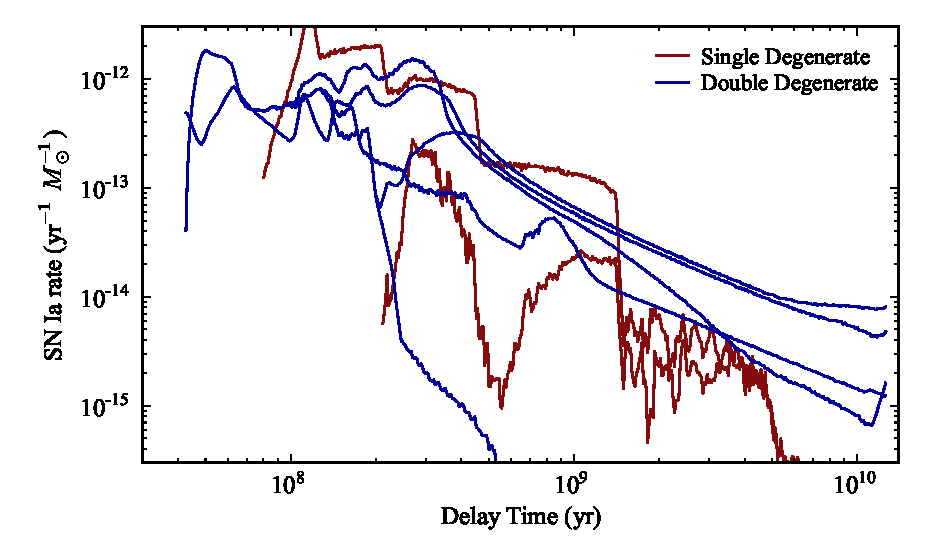
\includegraphics[width=\textwidth]{figures/review/dtd_mennekens10a.eps}
\end{center}
\caption[Example of delay time distributions]{An example of delay time
  distributions calculated using stellar population synthesis models
  from \citet{mennekens10a}. The various single degenerate and double
  degenerate DTDs use different assumptions and prescriptions for
  common envelope evolution.\label{fig:dtd_mennekens10a}}
\end{figure}

\section{Constraints from SN~Ia Rates}

As the DTD is simply the SN~Ia rate as a function of time after star
formation, it can be measured empirically by measuring the SN rate in
stellar populations of many different ages. In practice, this is
difficult because the typical galaxy is made up of many stars of
different ages. When a SN~Ia explodes, it is usually impossible to
tell which particular population the SN came from.

Five years ago, we had very little information about the shape of the
DTD from an observational standpoint. It had been recognized much
earlier that the SN~Ia rate is higher in star-forming galaxies
\citep{vandenbergh90a}, implying that the DTD is largest at small
delay times. [In fact, even earlier this trend was suggested as a
  motivation for two distinct subsets of SNe~I by
  \citet{dallaporta73a}.] However, little detail was gained over the
next 15 years. Some recent measurements have confirmed the same trend
with larger samples \citep{mannucci05a}. This has lead to a
parameterization of the DTD with a ``two component'' model
\citep{scannapieco05a} in which one component is proportional to the
instantaneous star formation rate and the other component is
proportional to stellar mass:
\begin{equation}
\mathcal{R}_{\rm SN~Ia} (t) = A M_\star (t) + B \dot{M}_\star(t).
\end{equation}
Also known as the ``$A+B$'' model, this form is convenient for
predicting the SN rate in environments with varying amounts of recent
star formation, and its parameters can be measured with relative ease
\citep[e.g.,][]{sullivan06a}. However, it suffers from being
unphysical (the $B$ component implies a delay time of zero) and
lacking theoretical motivation.  Unfortunately, this simplified model
was often interpreted as evidence for two distinct populations of
progenitors \citep[e.g.,][]{mannucci06a}, even though a single
progenitor channel could easily reproduce the observed
data. Complicating the entire situation at the time, some measurements
produced results in contradiction with the existence of short
delay-time SNe~Ia.  For example, \citet{dahlen04a} found the
volumetric SN~Ia rate (discussed in greater detail below) to decrease
at $z \gtrsim 1$, implying a narrow DTD centered at $t \sim 3$~Gyr,
with no contribution from short-delay SNe \citep{strolger04a}.

Recently, more detailed measurements of the DTD have become possible
using a variety of methods. Several measurements have confirmed that
the delay time spans a wide range, from less than 100 Myr
\citep[e.g.,][]{aubourg08a} to many Gyr
\citep[e.g.,][]{schawinski09a}. Detailed spectroscopic host galaxy
information for a large SN sample has allowed better constraints on
stellar population ages \citep{brandt10a}. The DTD at intermediate
delay times has been accessed using early-type galaxies
\citep{totani08a}. The common wisdom arising from these measurements
is that the SN rate generally declines with time, and that SNe with
progenitor ages $\lesssim$ a few hundred Myr comprise perhaps
$\sim$50\% of all SNe~Ia. 

We now discuss two particular approaches to DTD measurements that are
the main subject of this thesis: volumetric rates and rates
specifically in galaxy clusters.


%This is consistent with volumetric SN~Ia rate measurements
%\citep[e.g.][]{neill06a,dilday10a,dahlen04a,poznanski07a,kuznetsova08a,
%dahlen08a}
%which show that the SN~Ia rate clearly increases with redshift over
%the range $0<z<1$.

%The SN rate may also depend on metallicity of the progenitors, so
%measurements in stellar populations of different metallicity may shed
%light too.

\subsection{The Volumetric Field Rate}

One particular method for measuring the DTD is to correlate the cosmic
star formation history (SFH) with the the cosmic SN~Ia rate as a
function of redshift \citep{yungelson00a}: the rate as a function of
cosmic time is simply the cosmic SFH convolved with the DTD. Knowing
the SFH to good accuracy and measuring the SN~Ia rate, one can work
out the DTD.

A decade ago, before this method had ever been implemented, it was not
always looked upon as having great promise. Mario Livio, for one, took
this view in his review of SN~Ia progenitors:
\begin{quote}
The progenitors can be identified from the observed frequency of SNe
Ia as a function of redshift, since different progenitor models
produce different redshift distributions. Personally, I think it would
be quite pathetic to have to resort to this possibility.
\begin{flushright}
-- Mario \citet{livio01a}
\end{flushright}
\end{quote}
However, in the intervening ten years, this method has gained
appeal. In part, this has been because direct detection methods (such
as spectroscopic detection of hydrogen in SNe~Ia) have still not
provided definitive answers as hoped. At the same time advances in SN
rate measurements and new methods for backing out the DTD have started
yielding constraints that are informing progenitor models
\citep[e.g.][]{vankerkwijk10a}.

A measurement of the volumetric SN~Ia rate is often a ``free''
byproduct of conducting a survey for SNe for cosmology
measurements. As a result, the rate has now been measured in many
different SN surveys at redshifts $0<z<1$
\citep[e.g.]{pain02a,neill07a}. For some time, a number of
measurements were in disagreement. However, with new precise results
at low redshift \citep{dilday10a,li10a} and the recently revised rates
from the IfA Deep survey \citep{rodney10a}, most measurements at $z<1$
have now come into agreement, and paint a consistent picture of a SN
rate increasing with redshift. These measurements are reaching the
precision necessary for a DTD measurement: the slope of the increase
at low redshift ($z \lesssim 0.3$) alone has recently been used to
constrain the DTD \citep{horiuchi10a}.  However, due to the difficulty
of detecting $z \gtrsim 1$ SNe from the ground, measurements at these
higher redshifts have been limited to SN searches in the
GOODS\footnote{Great Observatories Origins Deep Survey
  \citep{giavalisco04a}} fields
\citep{dahlen04a,kuznetsova08a,dahlen08a} using \emph{HST} and
ultra-deep single-epoch searches in the Subaru Deep Field (SDF) from
the ground \citep{poznanski07a,graur11a}. These studies have yielded
discrepant results for both the SN rate and the implications for the
DTD. The first $z>1$ measurements by \citet{dahlen04a} \citep[and
  later][with an expanded dataset]{dahlen08a} showed a rate that
peaked at $z \sim 1$ and decreased in the highest redshift bin at
$z>1.4$. However, an independent analysis of much of the same dataset
by \citet{kuznetsova08a} resulted in a substantially lower rate at $z
\sim 1$ and an inability to distinguish a falling rate at high
redshift. The recent results of \citet{graur11a} from the SDF also
show a substantially lower rate at $z \sim 1$, at the level of
$\sim$$2\sigma$ (statistical-only) in each of two bins compared to
\citet{dahlen04a}. Their results are consistent with a flat SN rate at
$z \gtrsim 1$, and were used to infer a DTD proportional to a power
law in time with index of approximately $-1$.

Relative to the \emph{HST} measurements, the SDF measurements have the
advantage of better statistics in the highest-redshift bin,
but \emph{HST} measurements hold advantages in systematics.  A rolling
search with \emph{HST} offers multiple observations of each SN and
much higher resolution than possible from the ground, useful for
resolving separation between SNe and their hosts. These factors lead
to a more robust identification of SNe~Ia relative to the SDF searches
where a single observation is used for both detection and photometric
typing. In addition, the \citet{dahlen08a} analysis used spectroscopic
typing in addition to photometric typing, whereas \citet{graur11a}
uses only photometric typing. In general, the very different
strategies employed make \emph{HST} measurements a good cross-check
for the SDF measurements and vice versa. Increasing the statistics
in \emph{HST} rate measurements can help in resolving the source of
the discrepancies between the two measurements. At the same time, it
is important to carefully consider the assumptions about SN properties
that have gone into each measurement. Illustrating this importance is
the significant difference between the results
of \citet{kuznetsova08a} and \citet{dahlen08a} despite a largely
overlapping dataset.

In chapter~\ref{sec:fieldrate} of this thesis, we address these issues
by (1) supplementing current determinations of the \emph{HST}-based $z
\gtrsim 1$ SN~Ia rate and (2) comparing the effect on results of
different dust distributions assumed in previous analyses.


\subsection{Cluster Rates}

As an alternative to volumetric SN~Ia rates where stellar populations
with a wide range of ages contribute at all redshifts, it is more
straightforward to extract the DTD in stellar populations with a
narrow range of ages (with a single burst of star formation being the
ideal). Galaxy clusters, which are dominated by early-type galaxies,
provide an ideal environment for constraining the shape of the DTD at
large delay times. Early-type galaxies are generally expected to have
formed early ($z \gtrsim 2$) with little star formation since
\citep{stanford98a,vandokkum01a}. Cluster early-type galaxies in
particular form even earlier than those in the field, with most star
formation occurring at $z \gtrsim 3$
\citep{thomas05a,sanchezblazquez06a,gobat08a}.  Measuring the cluster
SN~Ia rate over a range of redshifts from $z=0$ to $z>1$ provides a
measurement of the SN~Ia rate at delay times from $\sim$2 to 11
Gyr. Obtaining an accurate rate at the highest-possible redshift is
crucial for constraining the shape of the late-time DTD: a larger
redshift range corresponds to a larger lever arm in delay time.

In addition to DTD constraints, there are also strong motivations for
measuring the cluster SN~Ia rate from a perspective of cluster
studies. SNe~Ia are an important source of iron in the intracluster
medium \citep[e.g.,][]{loewenstein06a}. Cluster SN rates constrain the
iron contribution from SNe and, paired with measured iron abundances,
can also constrain possible enrichment mechanisms \citep{maoz04a}. The
high-redshift cluster rate is particularly important: measurements
show that most of the intracluster iron was produced at high
redshift \citep{calura07a}. The poorly-constrained high-redshift
cluster rate is one of the largest sources of uncertainty in
constraining the metal-loss fraction from galaxies \citep{sivanandam09a}.

Cluster SNe~Ia can also be used to trace the
diffuse \emph{intracluster} stellar component. Intracluster stars,
bound to the cluster potential rather than individual galaxies, have
been found to account for anywhere from $5\%$ to $50\%$ of the stellar
mass in clusters \citep[e.g.,][]{ferguson98a,feldmeier98a,
gonzalez00a,feldmeier04a,lin04a,zibetti05a,gonzalez05a,krick06a,mihos05a}.
The use of SNe~Ia as tracers of this component was first demonstrated
by \citet{galyam03a} who found two likely host-less SNe~Ia out of a
total of seven cluster SNe~Ia in $0.06 < z < 0.19$ Abell
clusters. After correcting for the greater detection efficiency of host-less
SNe, they determined that on average, the intracluster medium
contained $20^{+20}_{-12}$\% of the total cluster stellar mass.  The
intrinsic faintness of the light from intracluster stars, combined
with $(1+z)^4$ surface brightness dimming, makes surface brightness
measurements impossible at redshifts much higher than $z=0.3$.  Type
Ia supernovae, which are detectable up to and beyond $z=1$, provide a
way to measure the intracluster stellar component and its possible
evolution with redshift.

The cluster SN~Ia rate has recently been measured at lower redshifts
($z>0.3$) in several studies \citep{sharon07a,mannucci08a,dilday10b},
and at intermediate redshift ($z\sim 0.6$) by
\citet{sharon10a}. However, at higher redshifts ($z \gtrsim 0.8$),
only weak constraints on the high-redshift cluster Ia rate exist,
based on 1--2 SNe~Ia at $z=0.83$ \citep{galyam02a}.  In
Chapter~\ref{sec:clrate} of this thesis, we calculate the SN~Ia rate
in $0.9 < z < 1.46$ clusters. We address the host-less SN~Ia fraction,
and use our result to place constraints on the late-time DTD in
clusters.

\section{Conventions Used in this Work}

Throughout this thesis a cosmology with
$H_0=70$~km~s$^{-1}$~Mpc$^{-1}$, $\Omega_M=0.3$, $\Omega_\Lambda =
0.7$ is assumed. Unless otherwise noted, magnitudes are in the Vega
system.


%%%%%%%%%%%%%%%%%%%%%%%%%%%%%%%%%%%%
% Chapter 2: HST Cluster SN Survey %
%%%%%%%%%%%%%%%%%%%%%%%%%%%%%%%%%%%%
\chapter{The \emph{HST} Cluster Supernova Survey} \label{sec:survey}

In a collaboration with members of the IRAC Shallow Cluster Survey
\citep{eisenhardt08a}, the Red-Sequence Cluster Survey (RCS) and RCS-2
\citep{gladders05a,yee07a}, the XMM Cluster Survey \citep{sahlen09a},
the Palomar Distant Cluster Survey \citep{postman96a}, the XMM-Newton
Distant Cluster Project \citep{bohringer05a}, and the ROSAT Deep
Cluster Survey \citep[RDCS;][]{rosati99a}, the SCP developed and
carried out a novel supernova survey approach. We aimed to improve
both the efficiency and usefulness of high-redshift SN observations
with \emph{HST} by specifically targeting high-redshift galaxy
clusters. Clusters provide a significant enhancement in the density of
potential SN hosts in \emph{HST}'s relatively small field of view.
Furthermore, the centers of rich clusters are dominated by relatively
dust-free early-type galaxies. SNe discovered in such galaxies offer
an opportunity to reduce the systematic uncertainty associated with
extinction corrections. Here we summarize the survey, named
the \emph{HST} Cluster Supernova Survey (PI Perlmutter; \emph{HST}
program GO-10496) and discuss aspects most relevant to the SN rate
calculation.

\section{Cluster Targets and Survey Strategy}

We used the Advanced Camera for Surveys (ACS) to search for and
observe SNe in 25 of the most massive galaxy clusters available at the
time of the survey. The survey was carried out during \emph{HST} Cycle
14 with observations spanning from July 2005 to December 2006.
Clusters were selected from X-ray, optical and IR surveys and cover
the redshift range $0.9<z<1.46$. Twenty-four of the clusters have
spectroscopically confirmed redshifts and the remaining cluster has a
photometric redshift estimate.  Cluster positions, redshifts and
discovery methods are listed in Table~\ref{tab:clusters}.

%%%%%%%%%%%%%%%%%%% 
% TABLE: CLUSTERS %
%%%%%%%%%%%%%%%%%%%
\begin{table}[thbp]
\caption{Clusters targeted in survey\label{tab:clusters}}
\begin{center}
\begin{footnotesizetabular}{lccccc}
\hline
\hline
ID & Cluster & Redshift & R.A. (J2000) & Decl. (J2000) & Discovery \\
\hline
A & XMMXCS J2215.9-1738 & 1.45 & $22^{\rm h}\,15^{\rm m}\,59^{\rm s}.0$ & $-17^{\circ}\,37'\,59''$ & X-ray      \\
B & XMMU J2205.8-0159   & 1.12 & $22^{\rm h}\,05^{\rm m}\,50^{\rm s}.6$ & $-01^{\circ}\,59'\,30''$ & X-ray      \\
C & XMMU J1229.4+0151   & 0.98 & $12^{\rm h}\,29^{\rm m}\,29^{\rm s}.2$ & $+01^{\circ}\,51'\,21''$ & X-ray      \\
D & RCS J0221.6-0347    & 1.02 & $02^{\rm h}\,21^{\rm m}\,42^{\rm s}.2$ & $-03^{\circ}\,21'\,52''$ & Optical    \\
E & WARP J1415.1+3612   & 1.03 & $14^{\rm h}\,15^{\rm m}\,11^{\rm s}.1$ & $+36^{\circ}\,12'\,03''$ & X-ray      \\
F & ISCS J1432.4+3332   & 1.11 & $14^{\rm h}\,32^{\rm m}\,28^{\rm s}.1$ & $+33^{\circ}\,33'\,00''$ & IR-Spitzer \\
G & ISCS J1429.3+3437   & 1.26 & $14^{\rm h}\,29^{\rm m}\,17^{\rm s}.7$ & $+34^{\circ}\,37'\,18''$ & IR-Spitzer \\
H & ISCS J1434.4+3426   & 1.24 & $14^{\rm h}\,34^{\rm m}\,28^{\rm s}.6$ & $+34^{\circ}\,26'\,22''$ & IR-Spitzer \\
I & ISCS J1432.6+3436   & 1.34 & $14^{\rm h}\,32^{\rm m}\,38^{\rm s}.8$ & $+34^{\circ}\,36'\,36''$ & IR-Spitzer \\
J & ISCS J1434.7+3519   & 1.37 & $14^{\rm h}\,34^{\rm m}\,46^{\rm s}.0$ & $+35^{\circ}\,19'\,36''$ & IR-Spitzer \\
K & ISCS J1438.1+3414   & 1.41 & $14^{\rm h}\,38^{\rm m}\,08^{\rm s}.2$ & $+34^{\circ}\,14'\,13''$ & IR-Spitzer \\
L & ISCS J1433.8+3325   & 1.37 & $14^{\rm h}\,33^{\rm m}\,51^{\rm s}.1$ & $+33^{\circ}\,25'\,50''$ & IR-Spitzer \\
M & Cl J1604+4304       & 0.92 & $16^{\rm h}\,04^{\rm m}\,23^{\rm s}.8$ & $+43^{\circ}\,04'\,37''$ & Optical    \\
N & RCS J0220.9-0333    & 1.03 & $02^{\rm h}\,20^{\rm m}\,55^{\rm s}.5$ & $-03^{\circ}\,33'\,10''$ & Optical    \\
P & RCS J0337.8-2844    & 1.1$^{\rm a}$ & $03^{\rm h}\,37^{\rm m}\,51^{\rm s}.2$ & $-28^{\circ}\,44'\,58''$ & Optical    \\
Q & RCS J0439.6-2904    & 0.95 & $04^{\rm h}\,39^{\rm m}\,37^{\rm s}.6$ & $-29^{\circ}\,05'\,01''$ & Optical    \\
R & XLSS J0223.0-0436   & 1.22 & $02^{\rm h}\,23^{\rm m}\,03^{\rm s}.4$ & $-04^{\circ}\,36'\,14''$ & X-ray      \\
S & RCS J2156.7-0448    & 1.07 & $21^{\rm h}\,56^{\rm m}\,42^{\rm s}.2$ & $-04^{\circ}\,48'\,04''$ & Optical    \\
T & RCS J1511.0+0903    & 0.97 & $15^{\rm h}\,11^{\rm m}\,03^{\rm s}.5$ & $+09^{\circ}\,03'\,09''$ & Optical    \\
U & RCS J2345.4-3632    & 1.04 & $23^{\rm h}\,45^{\rm m}\,27^{\rm s}.2$ & $-36^{\circ}\,32'\,49''$ & Optical    \\
V & RCS J2319.8+0038    & 0.91 & $23^{\rm h}\,19^{\rm m}\,53^{\rm s}.4$ & $+00^{\circ}\,38'\,13''$ & Optical    \\
W & RX J0848.9+4452     & 1.26 & $08^{\rm h}\,48^{\rm m}\,56^{\rm s}.4$ & $+44^{\circ}\,52'\,00''$ & X-ray      \\
X & RDCS J0910+5422     & 1.11 & $09^{\rm h}\,10^{\rm m}\,45^{\rm s}.1$ & $+54^{\circ}\,22'\,07''$ & X-ray      \\
Y & RDCS J1252.9-2927   & 1.23 & $12^{\rm h}\,52^{\rm m}\,54^{\rm s}.4$ & $-29^{\circ}\,27'\,17''$ & X-ray      \\
Z & XMMU J2235.3-2557   & 1.39 & $22^{\rm h}\,35^{\rm m}\,20^{\rm s}.8$ & $-25^{\circ}\,57'\,39''$ & X-ray      \\


\hline
\end{footnotesizetabular}
\end{center}
{\footnotesize

$^{\rm a}$ photometric redshift

{\bf References.} --- A \citep{stanford06a,hilton07a}; 
B,C \citep{bohringer05a,santos09a}; 
D \citep[also known as RzCS 052;][]{andreon08b,andreon08c}; 
D, N, U (Gilbank et al. in prep); E \citep{perlman02a};
F \citep{elston06a}; G, I, J, L \citep{eisenhardt08a}; 
L (Brodwin et al. in prep; Stanford et al. in prep);
H \citep{brodwin06a}; K \citep{stanford05a}; M \citep{postman01a};
Q \citep{cain08a}; R \citep{andreon05a,bremer06a};
S \citep{hicks08a}; V \citep{gilbank08a}; W \citep{rosati99a};
X \citep{stanford02a}; Y \citep{rosati04a}; 
Z \citep{mullis05a,rosati09a}.\\
{\bf Note.} --- Cluster positions differ slightly from those
originally reported in \citet{dawson09a} due to the use of an updated
algorithm for determining cluster centers. See \S\ref{sec:lum}
for a description of this algorithm.
}
\end{table}

During the survey, each cluster was observed once every 20 to 26 days
during its \emph{HST} visibility window (typically four to seven
months). Figure~\ref{fig:visits} shows the dates of visits to
each cluster. Each visit consisted of four exposures in the F850LP
filter (hereafter $z_{850}$).  Most visits also included a fifth
exposure in the F775W filter (hereafter $i_{775}$). We revisited
clusters D, N, P, Q, R and Z towards the end of the survey when they
became visible again.

%%%%%%%%%%%%%%%%
% PLOT: VISITS %
%%%%%%%%%%%%%%%%

\begin{SCfigure}[0.7][thb]
\centering
\includegraphics{figures/survey/visits.eps}
\caption[Dates of visits to each cluster]{Dates of visits to each
  cluster. All visits included $z_{850}$ exposures (usually
  four). Most visits also included one $i_{775}$ exposure. Filled
  circles indicate ``search'' visits (used for finding SNe). Open
  circles indicate ``follow-up'' visits (contingent on the existence
  of an active SN candidate). Clusters D, N, P, Q and R were
  re-visited once towards the end of the survey, with additional
  follow-up visits devoted to clusters in which promising SN
  candidates were found (N, Q, R). \label{fig:visits}}
\end{SCfigure}


Immediately following each visit, the four $z_{850}$ exposures were
cosmic ray-rejected and combined using {\sc MultiDrizzle}
\citep{fruchter02a,koekemoer02a} and searched for
supernovae. Following the technique employed in the earliest Supernova
Cosmology Project searches \citep{perlmutter95a,perlmutter97a}, we
used the initial visit as a reference image, flagged candidates with
software and then considered them by eye. Likely supernovae were
followed up spectroscopically using pre-scheduled time on the Keck
and Subaru telescopes and target-of-opportunity observations on VLT.
For nearly all SN candidates, either a live SN spectrum or host galaxy
spectrum was obtained. In many cases, spectroscopy of cluster galaxies
was obtained contemporaneously using slit masks. Candidates deemed
likely to be at higher redshift ($z>1$) were also observed with the
NICMOS camera on {\it HST}, but these data are not used in this work.

For the purpose of a rate calculation it is important to note that a
number of visits were contingent on the existence of an active SN. At
the end of a cluster's visibility window, the last two scheduled
visits were cancelled if there was no live SN previously
discovered. This is because a SN discovered on the rise in either of
the last two visits could not be followed long enough to obtain a
cosmologically useful light curve. In addition, supplementary visits
between pre-scheduled visits were occasionally added to provide more
complete light curve information for SNe (in the case of clusters A,
C, Q, and U). We call all visits contingent on the existence of an
active SN ``follow-up'' visits (designated by open circles in
Fig.~\ref{fig:visits}). Search and follow-up visits are considered
differently when calculating an SN rate.

\section{Data Processing}

Following the conclusion of the survey, all ACS images were
reprocessed \citep[see details in][]{suzuki11a}. This
reprocessing included an updated flat field, gain adjustment, custom
sky subtraction, and updated distortion correction and zeropoints.
The images for each cluster were aligned and output to a single common
reference frame for the cluster using the {\sc MultiDrizzle}
software. That is, the combined images for each epoch are all on the
same image and physical reference frame for a given cluster. This
makes it possible to stack and subtract images without resampling the
data. The four individual exposures (not cosmic ray-rejected) are also
transformed onto this output reference frame. The output pixel scale
is equal to the physical pixel scale: $0''.05$.

A single sky noise for each image is calculated, for use in the rate
calculation. To do this accurately, we first cut pixels with effective
exposure time less than 50\% of the total exposure time. We calculate
a rough sky noise level, then cut pixels belonging to objects. The
requirement to be an object is 1 pixel above $4\sigma$ and 5
contiguous pixels above $2.5\sigma$. This is done iteratively until
$\sigma$ has converged to within 25\%.

\section{Survey Publications}

The supernova-related results from the survey are reported in the
following publications: Paper I \citep{dawson09a} describes the survey
strategy and discoveries. Paper II \citep{barbary11a} reports on the
SN~Ia rate in clusters. Paper III \citep{meyers11a} addresses the
properties of the galaxies that host SNe~Ia. Paper
IV \citep{ripoche11a} introduces a new technique to calibrate the
zeropoint of the NICMOS camera at low counts rates, critical for
placing NICMOS-observed SNe~Ia on the Hubble diagram. Paper
V \citep{suzuki11a} reports the SNe~Ia light curves and cosmology from
the program. Paper VI (Barbary et al., in preparation) reports on the
volumetric field SN~Ia rate. \citet{melbourne07a}, one of several
unnumbered papers in the series, present a Keck adaptive optics
observation of a $z=1.31$ SN~Ia in $H$-band. \citet{barbary09a} report
the discovery of the extraordinary luminous supernova,
SN~SCP06F6. \citet{morokuma10a} presents the spectroscopic follow-up
observations for SN candidates. Finally, Hsiao et al. (in preparation)
develop techniques to remove problematic artifacts remaining after the
standard STScI pipeline. A separate series of papers, ten to date,
reports on cluster studies from the survey:
\citet{hilton07a,eisenhardt08a,jee09a,hilton09a,huang09a,rosati09a,
santos09a,strazzullo10a,brodwin10a}; Jee et al. (in preparation).


%%%%%%%%%%%%%%%%%%%%%%
% Chapter 3: SCP06F6 %
%%%%%%%%%%%%%%%%%%%%%%
\chapter{The Unusual Supernova SN SCP06F6} \label{sec:scp06f6}
Before we progress with the study of Type Ia SNe found in the survey,
we take a detour to discuss an very interesting transient that turned
out not to be a SN~Ia. The transient, designated either SN SCP06F6 or
SCP 06F6, was first detected in February 2006. It was originally
reported in a June 2006 IAU circular \citep{dawson06a} while detailed
data and a discussion were presented later in \citet{barbary09a}. Its
light curve rise-time of $\sim$100 days is inconsistent with all known
SN types, and its spectroscopic attributes are not readily matched to
any known variable. It is surprising to discover such a rare object in
a survey with \emph{HST}, given its extremely small field of view
relative to ground-based SN surveys. However, current indication are
that this is indeed what happened, as a few candidates bearing some
similarities have since been identified in vastly wider-area surveys.

%Supernova (SN) surveys are designed to detect the brightening of
%supernovae over timescales of days to weeks. They often cover large
%areas at high sensitivity. As a result, they are able to discover
%unusual and rare transients with similar timescales.  For example, in
%2006 the Lick Observatory Supernova Search (LOSS) discovered an
%optical transient in the galaxy M85 \citep{kulkarni07a,rau07b,ofek08a}
%with a light curve plateau of $\sim$80 days.  It is suggested that the
%origin of this transient is a stellar merger and that an entire class
%of similar transients, \emph{luminous red novae}, exists.  Other
%recent discoveries of rare objects include a Type Ia SN with a
%super-Chandrasekhar mass progenitor \citep{howell06a} from the
%Supernova Legacy Survey (SNLS) and SN 2005ap, the most luminous SN
%ever observed \citep{quimby07a} from the Texas Supernova Search
%(TSS).

We present photometry in \S\ref{sec:f6_phot} and spectroscopy in
\S\ref{sec:f6_spec}. In \S\ref{sec:f6_discussion}, we discuss
constraints on possible identities. 


\section{Photometry} \label{sec:f6_phot}

The transient was discovered on 21 February 2006 (UT) in a field
centered on cluster CL 1432.5+3332.8 (F; $z = 1.112$). This field was
imaged over nine epochs with a period of roughly three weeks.  The
 discovery occurred in the fourth epoch at a position $\alpha =
14^\mathrm{h} 32^\mathrm{m} 27^\mathrm{s}.40$, $\delta = +33^\circ 32'
24''.8$ (J2000.0).  The angular separation from the cluster center is
$35''$, corresponding to a projected physical separation at the
cluster redshift of 290 kpc.  Table~\ref{tab:lightcurve} gives a
summary of photometric observations.

There is no prior detection of a source at the transient's location in
the NRAO VLA Sky Survey \citep{condon98a} at 1.4~GHz to the survey
$5\sigma$ detection limit of 2.5~mJy beam$^{-1}$.  There is no X-ray
detection at this location in a 5 ks exposure in the Chandra Telescope
XBootes survey \citep{kenter05a} to the detection limit of $7.8 \times
10^{-15}~\mathrm{erg}~ \mathrm{cm}^{-2}~\mathrm{s}^{-1}$ in the full
0.5-7 keV band.

%%%%%%%%%%%%%%%%%%%%%%%%%%%%%%%%%%%%%%%%%%%%%%%%%%%%%%%%%%%%%%%%%%
% PHOTOMETRY TABLE                                               %
%%%%%%%%%%%%%%%%%%%%%%%%%%%%%%%%%%%%%%%%%%%%%%%%%%%%%%%%%%%%%%%%%%
\begin{table}[tbh]
\begin{center}
\caption{Photometric observations of SN SCP06F6\label{tab:lightcurve}}
\vspace{10pt}
\begin{footnotesizetabular}{l c c c c c c c}
\hline
\hline
     &       &     & Tele- &        & Exp. &             &           \\
Num. &  Date & MJD & scope & Filter & (s)  & Scaled Flux & Magnitude \\
\hline
1  & 11/28/05 & 53716.1 & \emph{HST} & $i_{775}$ & $175$  & $\phantom{-}0.0018 \pm 0.0049$  & $> 26.515$ \\
   &          &         &            & $z_{850}$ & $1400$ & $-0.0019 \pm 0.0053$            & $> 27.222$ \\
2  & 01/03/06 & 53738.7 & \emph{HST} & $i_{775}$ & $375$  & $\phantom{-}0.0002 \pm 0.0025$  & $> 27.509$ \\
   &          &         &            & $z_{850}$ & $1500$ & $\phantom{-}0.0053 \pm 0.0049$  & $26.733 \pm  0.857$ \\
3  & 01/29/06 & 53764.6 & \emph{HST} & $z_{850}$ & $1500$ & $\phantom{-}0.0087 \pm 0.0050$  & $26.185 \pm  0.524$ \\
4  & 02/21/06 & 53787.2 & \emph{HST} & $i_{775}$ & $515$  & $\phantom{-}0.1183 \pm 0.0032$  & $23.395 \pm  0.025$ \\
   &          &         &            & $z_{850}$ & $1360$ & $\phantom{-}0.1367 \pm 0.0059$  & $23.201 \pm  0.040$ \\
5  & 03/19/06 & 53813.7 & \emph{HST} & $i_{775}$ & $440$  & $\phantom{-}0.4229 \pm 0.0055$  & $22.012 \pm  0.012$ \\
   &          &         &            & $z_{850}$ & $1360$ & $\phantom{-}0.3805 \pm 0.0067$  & $22.089 \pm  0.016$ \\
6  & 04/04/06 & 53829.6 & \emph{HST} & $i_{775}$ & $515$  & $\phantom{-}0.6216 \pm 0.0065$  & $21.593 \pm  0.010$ \\
   &          &         &            & $z_{850}$ & $1360$ & $\phantom{-}0.6055 \pm 0.0074$  & $21.585 \pm  0.011$ \\
7  & 04/22/06 & 53847.0 & \emph{HST} & $i_{775}$ & $515$  & $\phantom{-}0.8343 \pm 0.0068$  & $21.274 \pm  0.008$ \\
   &          &         &            & $z_{850}$ & $1360$ & $\phantom{-}0.8276 \pm 0.0080$  & $21.246 \pm  0.009$ \\
8  & 05/21/06 & 53876.8 & \emph{HST} & $i_{775}$ & $295$  & $\phantom{-}1.0000 \pm 0.0099$  & $21.077 \pm  0.009$ \\
   &          &         &            & $z_{850}$ & $1400$ & $\phantom{-}1.0000 \pm 0.0082$  & $21.040 \pm  0.008$ \\
9  & 06/03/06 & 53889.3 & \emph{HST} & $i_{775}$ & $800$  & $\phantom{-}0.8534 \pm 0.0056$  & $21.249 \pm  0.006$ \\
   &          &         &            & $z_{850}$ & $1200$ & $\phantom{-}0.9176 \pm 0.0081$  & $21.134 \pm  0.008$ \\
10 & 06/28/06 & 53914.4 & Subaru     & $i_{775}$ & $960$  & $\phantom{-}0.6290 \pm 0.1441$  & $21.581 \pm  0.211$ \\
   &          &         &            & $z_{850}$ & $480$  & $\phantom{-}0.7384 \pm 0.1520$  & $21.370 \pm  0.189$ \\
11 & 08/23/06 & 53970.3 & Subaru     & $i_{775}$ & $600$  & $\phantom{-}0.0586 \pm 0.0234$  & $24.158 \pm  0.368$ \\
   &          &         &            & $z_{850}$ & $600$  & $\phantom{-}0.0654 \pm 0.0875$  & $> 23.080$ \\
12 & 05/18/07 & 54238.5 & Subaru     & $i_{775}$ & $2280$ & $-0.0324 \pm 0.0201$            & \ldots \\
\hline
\end{footnotesizetabular}

\end{center}
{\footnotesize
{\bf Note.} --- Flux measurements scaled relative to highest flux
epoch; effective zeropoints are 21.077 for $i_{775}$ and 21.040 for
$z_{850}$.
}
\end{table}

%%%%%%%%%%%%%%%%%%%%%%%%%%%%%%%%%%%%%%%%%%%%%%%%%%%%%%%%%%%%%%%%%%
% IMAGE                                                          %
%%%%%%%%%%%%%%%%%%%%%%%%%%%%%%%%%%%%%%%%%%%%%%%%%%%%%%%%%%%%%%%%%%
\begin{figure}
\begin{center}
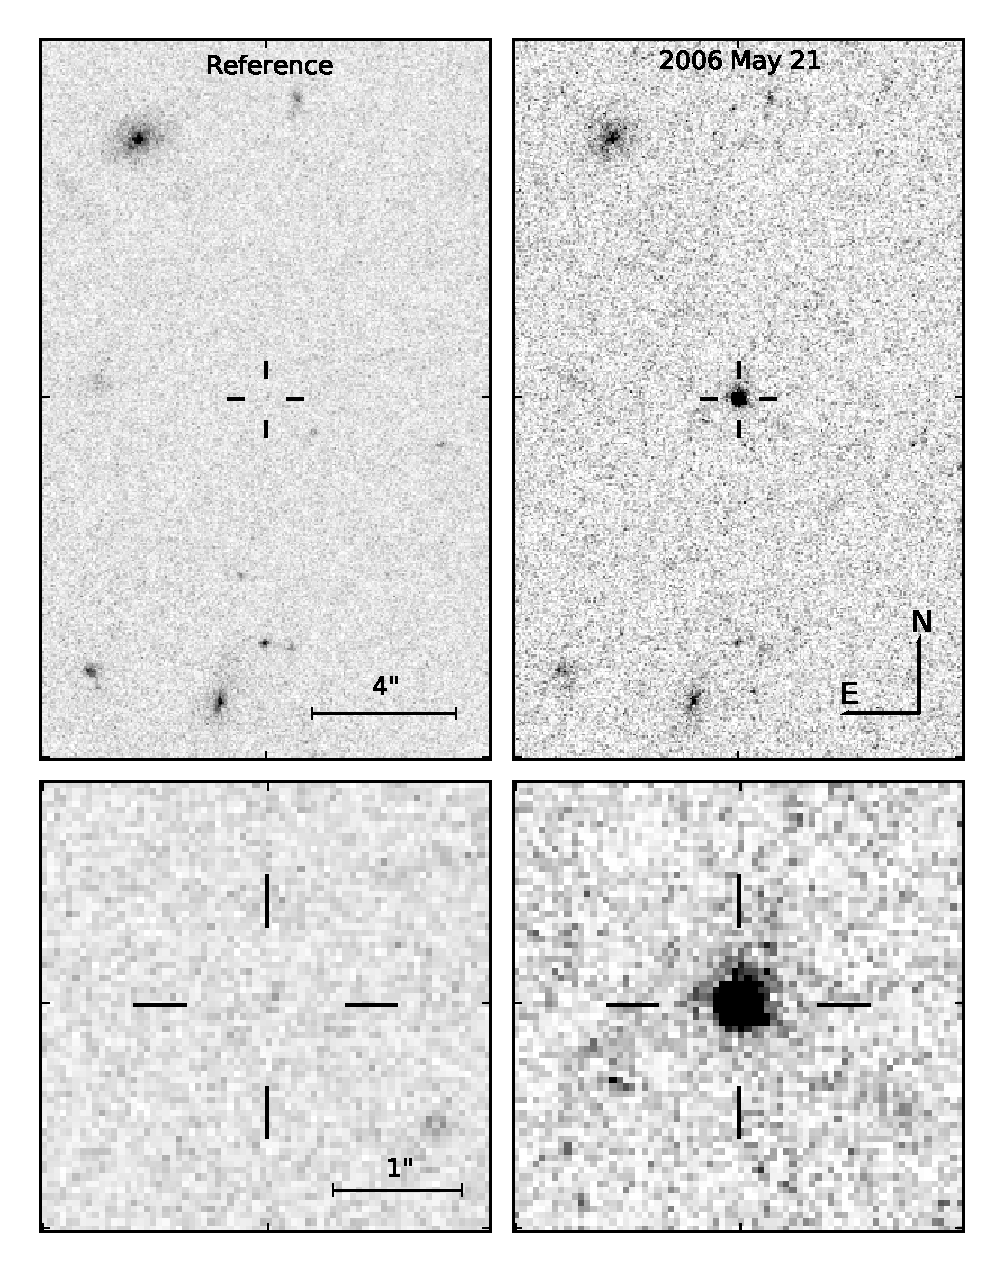
\includegraphics[width=0.9\textwidth]{figures/scp06f6/images.eps}
\end{center}
\caption[Imaging of SN SCP06F6]{Deep stack of the first three epochs
  in $z_{850}$ totaling 4400~s where the transient is undetected
  (\emph{top left} and zoomed in, \emph{bottom left}), and the
  highest-flux epoch eight $z_{850}$ exposure of 1400~s (\emph{top
    right} and zoomed in, \emph{bottom right}).  All images have the
  same greyscale.  The hash marks indicate the transient position and
  have the same physical scale in all images.\label{fig:images}}
\end{figure}

%%%%%%%%%%%%%%%%%%%%%%%%%%%%%%%%%%%%%%%%%%%%%%%%%%%%%%%%%%%%%%%%%%
% LIGHTCURVE PLOT                                                %
%%%%%%%%%%%%%%%%%%%%%%%%%%%%%%%%%%%%%%%%%%%%%%%%%%%%%%%%%%%%%%%%%%
\begin{figure}
\begin{center}
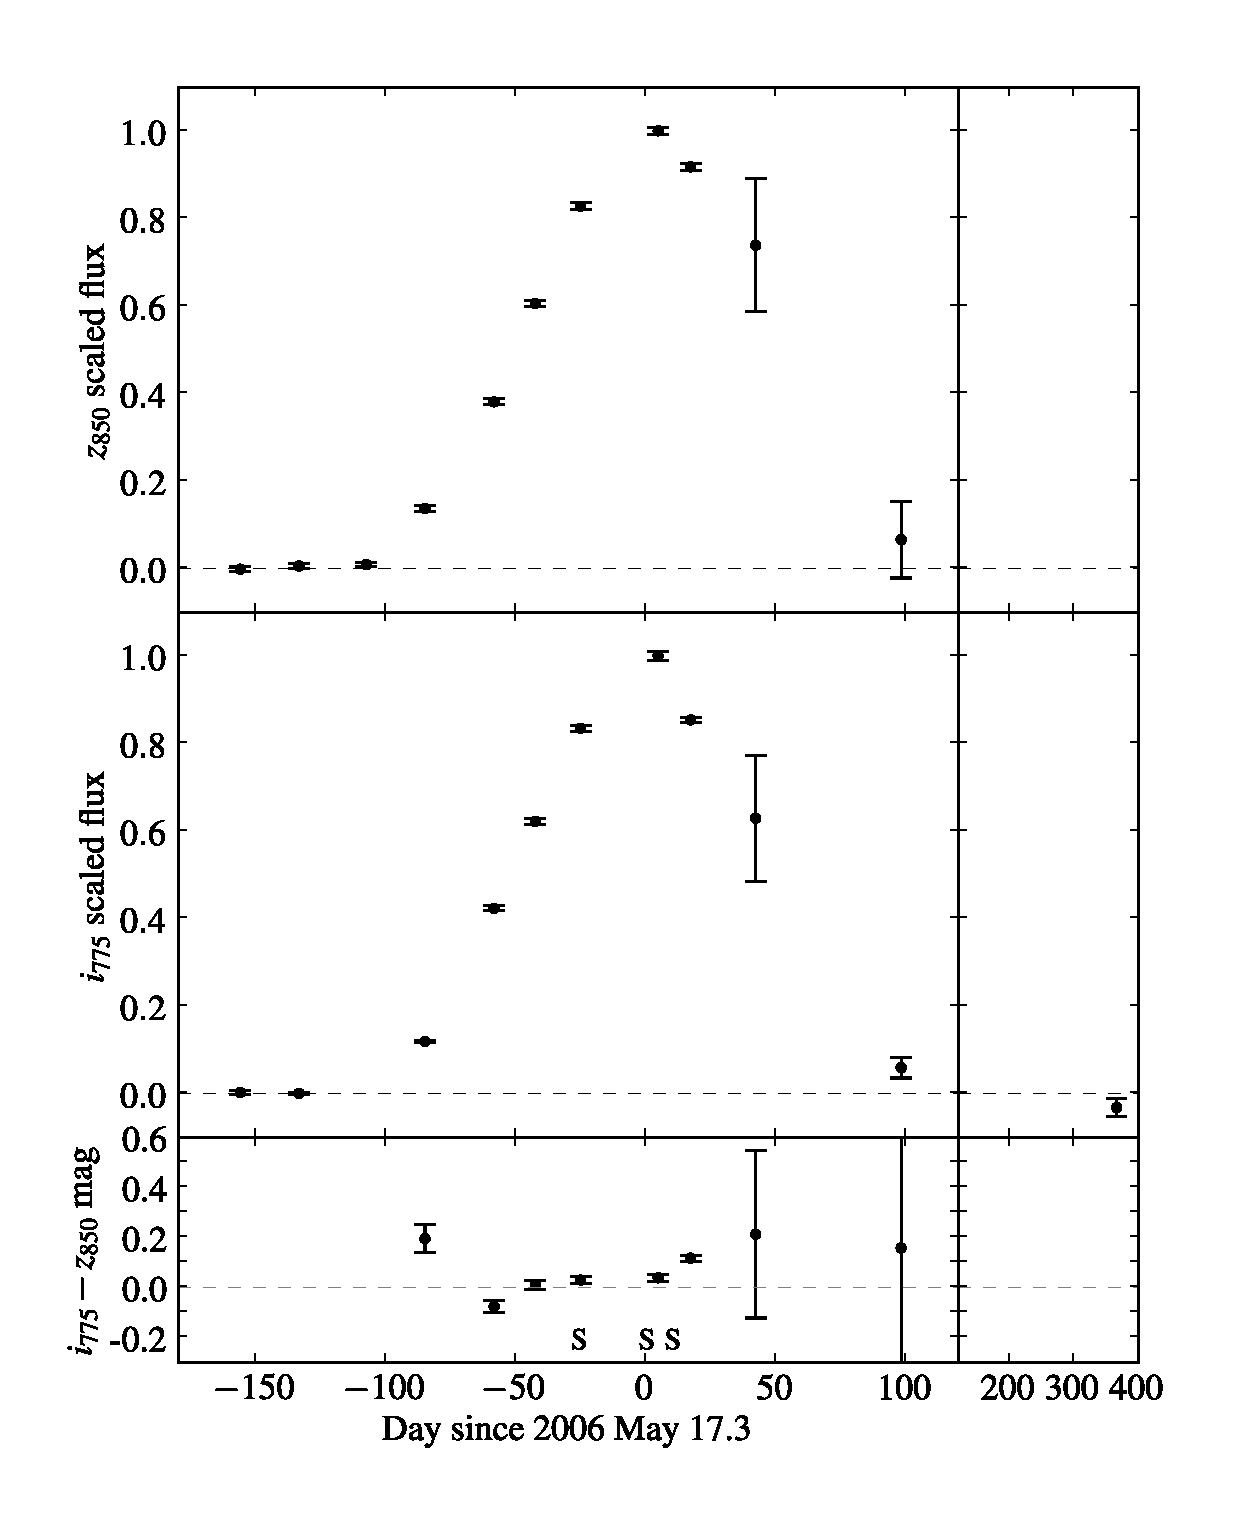
\includegraphics[width=0.9\textwidth]{figures/scp06f6/lightcurve.eps}
\end{center}
\caption[Light curve of SN SCP06F6]{Flux light curve for $z_{850}$
  (\emph{top panel}) and $i_{775}$ (\emph{middle panel}) scaled to
  maximum flux.  The last three epochs (starting at +42 days) are
  Subaru FOCAS observations.  \emph{bottom panel}: $i_{775} - z_{850}$
  color for epochs with significant detection in both bands. Though
  the color only varies $\sim 0.2$ magnitudes between the five best
  measured epochs, there is evidence for evolution.  The spectral
  epochs are marked along the abscissa with an ``S.''
	 \label{fig:lightcurve}}
\end{figure}

The transient is consistent with a point source in each of the six ACS 
detection epochs to the extent we can determine.
We performed aperture photometry on the {\sc MultiDrizzle}-processed ACS images
using 3.0 pixel ($0''.15$) radius apertures for $i_{775}$ and 5.0~pixel 
($0''.25$) radius apertures for $z_{850}$. Aperture corrections were taken 
from Table~3 of \citet{sirianni05a}. The systematic error due to the known 
color dependence of $z_{850}$ aperture correction \citep[see][]{sirianni05a} 
is estimated to be less than 0.015~mag.

After the transient had left the visibility window of \emph{HST} it remained 
visible from Mauna Kea for several months. Three additional photometry points 
were obtained with the Faint Object Camera and Spectrograph 
\citep[FOCAS;][]{kashikawa02a} 
on the Subaru telescope on 2006 June 28, 2006 August 23, 
and the next year on 2007 May 18. The June observations suffered from poor 
weather conditions (seeing $\gtrsim 2''$). 
All observations were cosmic ray-rejected using 120~s exposures. 
We performed aperture photometry using a $1''.04$ radius aperture and 
estimated photometric errors as described by \citet{morokuma08a}. 
In order to express magnitudes in the ACS filter 
system, we determined Subaru image zeropoints by cross-correlating the 
photometry of nine surrounding stars in the ACS and Subaru images. The 
Subaru FOCAS $i'$ and $z'$ filters are similar enough to ACS $i_{775}$ and 
$z_{850}$ that there is no significant trend with stellar color.

A deep stack of the first three epochs in $z_{850}$ totaling 4400~s 
(Fig.~\ref{fig:images}) and first two epochs 
in $i_{775}$ totaling 550~s provide limits on the magnitude of a possible 
progenitor star (if galactic) or host galaxy (if extragalactic).
No progenitor star is detected in a 3.0~pixel radius aperture centered at the 
position of the transient (known to $< 0.2$~pixels) to a $3\sigma$ upper limit 
of $i_{775} > 26.4$ and $z_{850} > 26.1$ 
(Vega magnitudes are used throughout this Letter).
There is no sign of a host galaxy in the 1~arcsec$^2$ surrounding the 
transient to a surface brightness $3\sigma$ limit of 25.0~mag~arcsec$^{-2}$ and 
25.1~mag~arcsec$^{-2}$ in $z_{850}$ and $i_{775}$, respectively.
However, there is a $6\sigma$ detection in a 3.0~pixel radius aperture of a 
$\sim$25.8~mag object $1''.5$ southwest of the 
transient position in $z_{850}$ (Fig.~\ref{fig:images}, \emph{lower left}). 
If the transient is extragalactic, this might represent a faint host galaxy.

The transient increased in brightness in each of 
epochs four through eight before finally declining in the ninth epoch, 
resulting in a rise time of approximately 100~days 
(Fig. \ref{fig:lightcurve}). 
A fit to the brightest five ACS $z_{850}$ photometry points 
gives a date of max of 2006 May 17.3 (MJD 53872.3). 
The declining part of the light curve, although sparsely measured, 
is consistent with symmetry about the maximum. 
The final photometry point approximately one year after maximum light shows 
no detection. The $i_{775} - z_{850}$ color is approximately constant over 
the 50~days preceding maximum light, but does show significant signs of 
evolution at early times and after maximum light.


\section{Spectroscopy} \label{sec:f6_spec}

%%%%%%%%%%%%%%%%%%%%%%%%%%%%%%%%%%%%%%%%%%%%%%%%%%%%%%%%%%%%%%%%%%
% SPECTROSCOPY PLOT                                              %
%%%%%%%%%%%%%%%%%%%%%%%%%%%%%%%%%%%%%%%%%%%%%%%%%%%%%%%%%%%%%%%%%%
\begin{figure}
\begin{center}
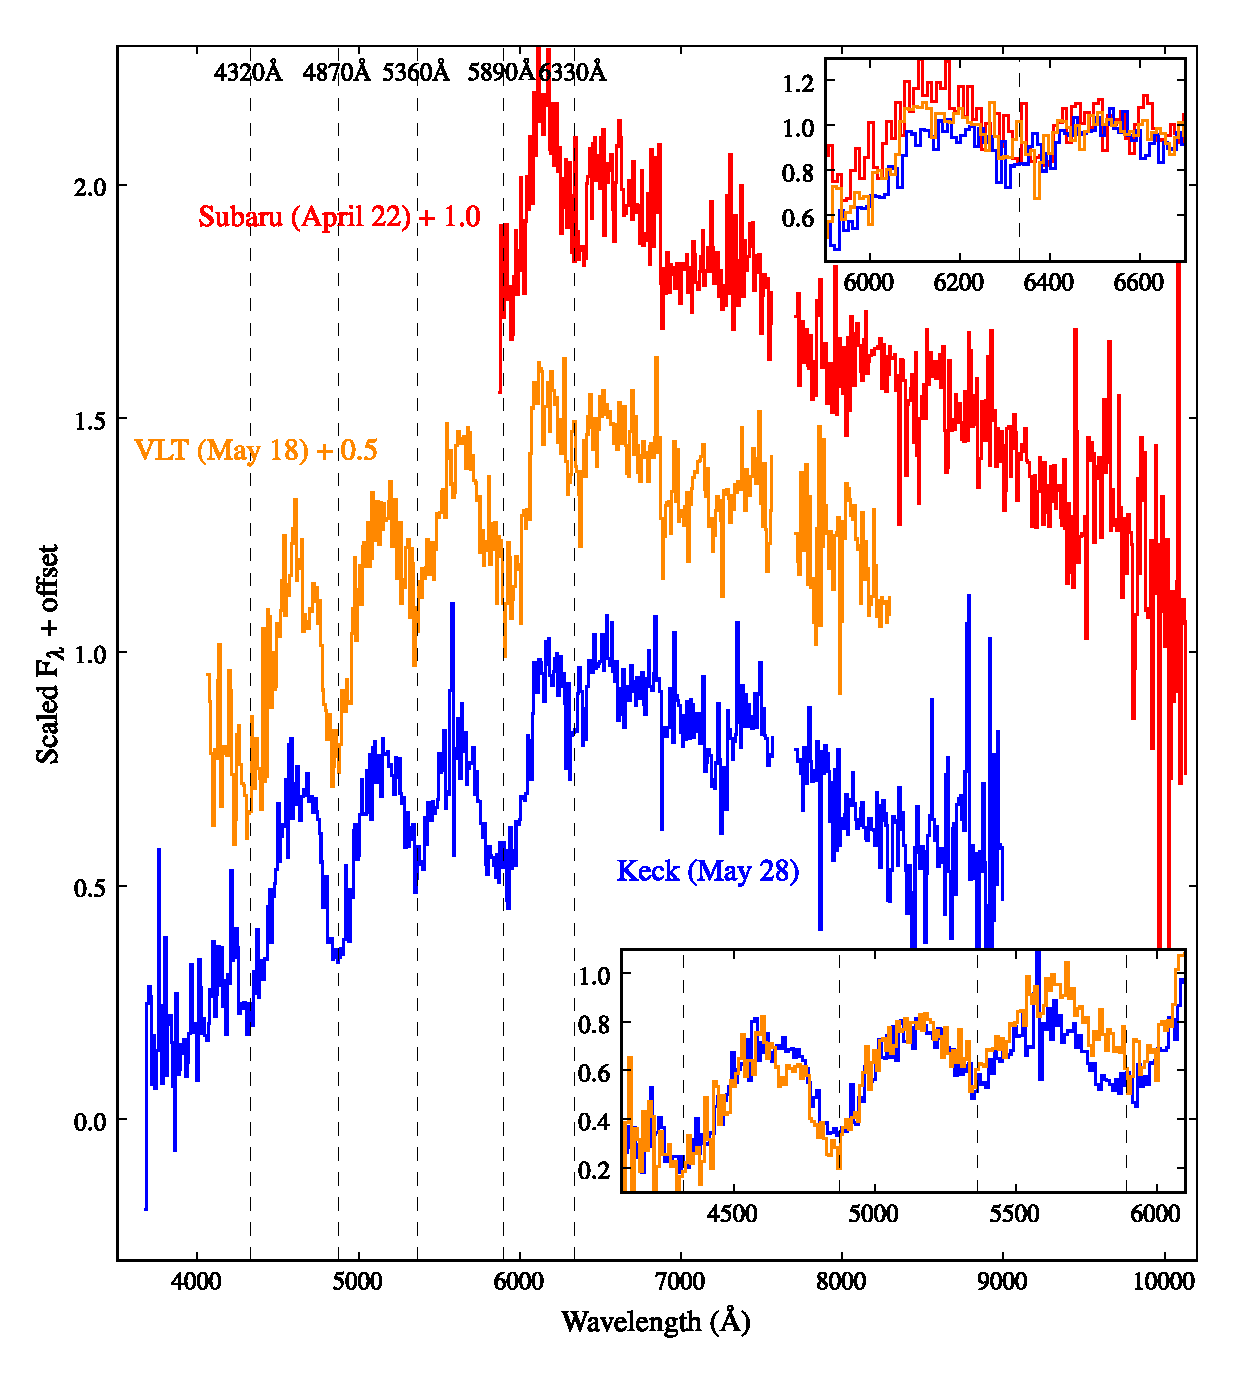
\includegraphics[width=\textwidth]{figures/scp06f6/spectra.eps}
\end{center}
\caption[Spectroscopy of SN SCP06F6]{Spectra averaged in
  10~\AA\ bins. Vertical dotted lines indicate the approximate
  absorption band centroids. Spectra are normalized to match in the
  red continuum. Inset figures show regions where spectra differ.
  \emph{Top Inset}: Overplot of all three spectra in the range
  5900~\AA\ - 6700~\AA, demonstrating apparent evolution of the flux
  at $\sim$6150~\AA\ relative to the red continuum.  \emph{Bottom
    Inset}: Overplot of VLT and Keck spectra (no offset) demonstrating
  apparent evolution at 4670~\AA\ and of the absorption feature at
  5890~\AA.\label{fig:spectra}}
\end{figure}

Spectroscopy was acquired on three dates (Fig.~\ref{fig:spectra}): 
2006 April 22 (-25~days) using Subaru FOCAS, 
2006 May 18 (+1~day) using VLT FORS2 \citep{appenzeller98a}, and 
2006 May 28 (+11~days) with Keck LRIS \citep{oke95a}.
The Subaru spectrum covers wavelengths longward of 5900~\AA, 
while the VLT and Keck spectra cover bluer wavelengths.
The VLT spectrum (observed at airmass $> 2$) is corrected for differential 
slit loss by applying a linear correction with a slope of 0.25 per 1000~\AA, 
derived from a comparison to the Keck spectrum, which covers the 
entire wavelength range of the VLT spectrum.
The Keck observation was made at the parallactic angle, 
while Subaru FOCAS is equipped with an atmospheric dispersion corrector,
making these observations more reliable measures of relative flux.

The spectra show a red continuum and several broad absorption features: 
a possible absorption feature at 4320~\AA\ ($\mathrm{FWHM} \sim 180$~\AA), 
three strong features at 4870~\AA\ ($\mathrm{FWHM} \sim 200$~\AA), 
5360~\AA\ ($\mathrm{FWHM} \sim 230$~\AA) and 5890~\AA\ 
($\mathrm{FWHM} \sim 280$~\AA), 
and a weaker absorption feature at 6330~\AA\ ($\mathrm{FWHM} \sim 270$~\AA). 
Including uncertainty in continuum shape, errors are estimated to be 25~\AA.

We compared the spectra to all supernova types using the $\chi^2$ fitting 
program described in \citet{howell05a} as well as the program SNID 
\citep{blondin07a}. No match was found with either program.

If the transient is galactic ($z=0$),
the absorption features at 4320~\AA\ and 4870~\AA\ are consistent with
$\mathrm{H}\gamma$ (4341~\AA) and $\mathrm{H}\beta$ (4861~\AA) respectively.
However, there is no significant $\mathrm{H}\alpha$ (6563~\AA) emission or 
absorption, which would be expected for the presence of strong 
$\mathrm{H}\gamma$ and $\mathrm{H}\beta$ features. (Although there is 
slight evidence for emission at 6563~\AA\ in the 
Keck spectrum, this is not seen in the VLT or Subaru spectra.)
It is therefore unlikely that the 4320~\AA\ and 4870~\AA\ features are 
due to hydrogen.
No other narrowband emission or absorption lines are detected.
From the slope of the red continuum we derive a lower limit blackbody 
temperature of 6500 K. The shape of the continuum is inconsistent with 
$\mathrm{F}_\lambda \propto \lambda^{-5/3}$ synchrotron radiation. 

If the transient is extragalactic, the absence of Lyman $\alpha$ absorption 
features shortward of 4500 \AA\ places a hard upper limit of $z \lesssim 2.7$ on 
its redshift. Among redshifts $0 < z < 2.7$, the cluster redshift of 
$z = 1.112$ is of specific interest;
the transient is located a small projected distance from the center of the 
cluster. At this redshift,
the absorption feature at 5890~\AA\ is consistent with Mg \textsc{ii}
$\lambda\lambda2796,2803$. However, the remaining features are not identified 
at this redshift. At $z = 1.112$, a peak apparent magnitude of 
$i_{775} = 21.0$ implies a peak bolometric magnitude of approximately $-22.1$.

A comparison of the three spectra shows evidence for spectral evolution.
The flux at 
$\sim$6150~\AA\ consistently decreases relative to the red continuum over time
(Fig.~\ref{fig:spectra}, \emph{upper inset}).
Over the 10 day period from the VLT to the Keck spectrum, 
the absorption feature at 5890~\AA\ appears to move toward shorter wavelengths,
while a small absorption feature at 4670~\AA\ in the VLT spectrum 
seems to disappear in the Keck spectrum
(Fig.~\ref{fig:spectra}, \emph{lower inset}).


\section{Discussion} \label{sec:f6_discussion}

The key features of SN SCP06F6 are as follows: a rise time of
$\sim$100~days with a roughly symmetric light curve; small but
statistically significant color variations across the light curve; no
detected host galaxy or progenitor; broad spectral features in the
blue, with a red continuum, and some evidence for spectral evolution.
Below, we first discuss constraints on the distance to the source.
Next we consider the possibility that the transient is the result of
microlensing, finding this to be unlikely.  Lastly, we search for
objects in the SDSS spectral database, finding no convincing matches.

%%%%%%%%%%%%%%%%%%%%%%%%%%%%%%%%%%%%%%%%%%%%%%%%%%%%%%%%%%%%%%%%%%%%
% PROPER MOTION PLOT                                               %
%%%%%%%%%%%%%%%%%%%%%%%%%%%%%%%%%%%%%%%%%%%%%%%%%%%%%%%%%%%%%%%%%%%%
\begin{figure}[tbh]
\begin{center}
\includegraphics[width=0.8\textwidth]{figures/scp06f6/propmotion.eps}
\end{center}
\caption[Proper motion of SN SCP06F6]{Position of the transient in
  each of the 6 ACS detection epochs.  1 pixel is $0''.05$. The upper
  limit on parallax is 0.3 pixels.\label{fig:propmotion}}
\end{figure}

\subsection{Distance from Parallax}
Any detection of proper motion or parallax would be strong evidence of
a galactic source. We tested for this by fitting the position of the
transient in each of the six ACS detection epochs using a
two-dimensional Gaussian (Fig.~\ref{fig:propmotion}).  The fit
uncertainty is dominated by residual distortion and alignment errors
in most epochs.  These errors are on the order of 0.1 to 0.2~pixels.
The most discrepant positions differ by approximately 0.25~pixels
($0''.0125$).  As a whole, the positions are consistent with no proper
motion or parallax and give little indication of either.  The upper
limit on parallax is 0.3~pixels ($0''.015$), which gives a lower limit
on distance of $\sim$70~pc.

\subsection{Distance from Reference Limits}
We can derive a more significant constraint on distance from reference
image magnitude limits, assuming that the transient is an explosion
and a progenitor star exists. The dimmest stars (aside from neutron
stars) known to undergo explosions are white dwarfs (WDs).  WDs range
in absolute magnitude from approximately 10~mag
($T_\mathrm{eff}\sim25000$~K) to approximately 16~mag
($T_\mathrm{eff}\sim3000$~K).  If we assume the progenitor is a WD
with absolute magnitude $i_{775} = 13$, the reference image $3\sigma$
upper limit of $i_{775} > 26.4$ gives a distance $3\sigma$ lower limit
of 4.8~kpc. Because the source is at high galactic latitude ($b =
67.3^\circ$), we are looking nearly directly out of the plane of the
galaxy. Given a Milky Way scale height for WDs of $(275 \pm 50)$~pc
\citep{boyle89a}, this places the source firmly outside of the plane
of the Galaxy. However, a galactic WD progenitor is still possible, if
it is a relatively cool white dwarf residing in the galactic halo. If
the progenitor is a source dimmer than $i_{775} = 13$~mag (e.g., a
cooler WD or neutron star), the constraints on distance are weaker.

\subsection{A Microlensing Event?}
Although the symmetry of the light curve (Fig.~\ref{fig:lightcurve})
suggests that the transient is a microlensing event, this
interpretation is unlikely.  The light curve is dramatically broader
than the theoretical light curve for microlensing of a point source by
a single lens \citep{paczynski86a}. The typical light curve FWHM of
high-magnification (peak magnification $\gtrsim 300$) microlensing
events is on the order of a few hours \citep[e.g.,][]{abe04a,dong06a}
whereas the transient's light curve FWHM is $\sim$100 days with a peak
magnification $3\sigma$ lower limit of $\sim$120.  Also, the color
evolves a small but significant amount over the light curve,
particularly between epochs eight and nine. Some of these difficulties
can be overcome if we assume the source is resolved; this can both
change the shape of the light curve and allow for color variation as
different source regions are differentially magnified. However, this
typically results in a lower peak magnification. Finally, microlensing
would still not explain the mysterious spectrum.

\subsection{Search for Similar Objects in SDSS}
In an effort to identify objects with similar spectra, we
cross-correlated the broad features of the spectrum with the SDSS
spectral database. Each SDSS spectrum was warped with a polynomial
function to best fit the Keck spectrum, based on a least squares
fit. The value of the root mean square of the difference between the
spectra was used to determine the correlation. An allowance for
relative redshift was made, with the requirement that the spectra
overlapped in the range of the strongest features (3500~\AA\ to
6200~\AA). No convincing matches were found. Changing the warping
function between linear and quadratic and varying the wavelength range
used in the fit altered which SDSS objects had the highest
correlation, but did not result in a more convincing match. The SDSS
objects with the highest correlation were broad absorption line
quasars (BAL QSOs) at various redshifts and carbon (DQ) WDs.  Although
BAL QSOs do have similarly broad features, they don't exhibit the
spacing or rounded profiles of those of the transient. Also, BAL QSOs
typically include emission features. The DQ WDs most similar to the
transient are known as DQp WDs. Like the transient, DQp WDs have
broad, rounded absorption features between 4000~\AA\ and
6000~\AA\ with a red continuum \citep[see, e.g.,][]{hall08a}. However,
the positions and spacing of the absorption features shortward of
5000~\AA\ differ greatly from those of the transient spectrum. In
addition, DQp WDs show increased emission toward the UV, which is not
seen in the transient.

The absence of similar spectra in the SDSS database implies that if
the transient is due to a galactic variable, it is either always below
the SDSS detection threshold in quiescence or extremely rare, or both.
If the transient is extragalactic, the apparent absence of similar
transients in other deep variable surveys (e.g., other high-redshift
supernova surveys) might be understood if similar transients are rare
at peak apparent magnitudes of 21 but more common at much fainter
magnitudes. 

\section{Summary}

Since the initial publication of this data, many possible scenarios
have been suggested to explain the observations.  Various explanations
have been considered by, e.g., \citet{gansicke09a}, \citet{soker10a}
and \citet{chatzopoulos09a}. It appears that the transient may be a
rare type of supernova, with redshift
$z=1.189$ \citep{quimby09a,pastorello10a}. However, its precise
explanation is still uncertain.


%%%%%%%%%%%%%%%%%%%%%%%%%%%%%%%%%%%%%%%%%%%%%%%%
% Chapter 4: SN Candidate Selection and Typing %
%%%%%%%%%%%%%%%%%%%%%%%%%%%%%%%%%%%%%%%%%%%%%%%%
\chapter{Supernova Candidate Selection and Typing} \label{sec:cands}

During the survey, our aim was to find as many supernovae as possible
and find them as early as possible in order to trigger spectroscopic
and NICMOS follow-up. Thus, software thresholds for flagging
candidates for consideration were set very low, and all possible
supernovae were carefully considered by a human screener. Over the
course of the survey, thresholds were changed and the roster of people
scanning the subtractions changed. As a result, the initial candidate
selection process was inclusive but heterogeneous, and depended
heavily on human selection. This made it difficult to calculate a
selection efficiency for the SN candidates selected during the
survey \citep[listed in Tables~3 and 4 of][]{dawson09a}. This is a
difficulty for a rate calculation since knowing the survey selection
efficiency is fundamental to calculating an accurate rate.

Therefore, in this chapter, we select an independent SN candidate sample
(without regard for the sample selected during the survey) using
automated selection wherever possible. Candidates are selected without
regard for cluster membership (which is only known from follow-up
spectroscopy once the candidate has already been found). We
determine SN types for both cluster and non-cluster SNe. The cluster
SNe are then considered further in Chapter~\ref{sec:clrate} in
calculating the cluster rate. The non-cluster SNe are considered
further in Chapter~\ref{sec:fieldrate} in calculating the volumetric
field rate.  The SN type determination here is also used to classify
candidates for use in the cosmological analysis from the
survey \citep{suzuki11a}.

The automated selection consists of initial detection in pairs of
subtracted images (\S\ref{sec:cands_search}; 86 candidates selected),
and subsequent requirements based on the light curve of each candidate
(\S\ref{sec:cands_lccuts}; 60 candidates remaining). The selection
efficiency for these two steps is later calculated via a Monte Carlo
simulation. In \S\ref{sec:cands_typing} we assign a type (SN~Ia,
core-collapse SN, or other) to each of the remaining 60 candidates
based on all data available (including triggered follow-up
observations). For this last step we do not calculate an efficiency or
completeness. Instead we estimate the classification uncertainty of
the assigned type for each candidate individually. For most candidates
the uncertainty in the type is negligible thanks to ample photometric
and spectroscopic data.


\section{Automated Selection}

\subsection{Initial Detection} \label{sec:cands_search}

%Reasons for only searching ``search'' visits:
%Using info that depends on a presence of a SN will create a bias. 
%Also, we don't want to consider supernovae found in the last visit to
%a cluster, as it would be very difficult to determine the type of a SN
%based on only one light curve point on the rise.

For the purpose of initially detecting candidates, we use only
``search'' visits (filled circles in Fig.~\ref{fig:visits}) and
disregard the ``follow-up'' visits (open circles in
Fig.~\ref{fig:visits}). (In the following section we will use any
available ``follow-up'' visits to construct more complete light curves
for the candidates discovered in this section.) We use the {\sc
MultiDrizzle}-combined, cosmic ray-rejected, $z_{850}$ image from each
``search'' visit. We consider only regions in this image that are
covered by three or more $z_{850}$ exposures.  With less than three
exposures, the combined images are too heavily contaminated by cosmic
rays to be practically searchable for SNe. Although there are
typically four $z_{850}$ exposures, the dither pattern used in the
survey means that not all regions of the combined image have four
exposures. The ACS camera is a mosaic of two $2048 \times 4096$~pixel
CCD chips (1~pixel = $0.05''$) separated by $2.5''$. The $z_{850}$
exposures were dithered to cover this gap, meaning that a $5''$ wide
region in the center of the image and $2.5''$ wide regions on either
side of the image are only covered by two exposures and thus are not
searchable. Due to orbital constraints, the position angle of {\it HST}
changes between each visit. This means that the unsearchable ``gap''
region rotates over the field between visits, and that the outer parts
of the field are observed in some visits, but not others
(Fig.~\ref{fig:epochs}, second row). The regions around bright stars
are also considered ``not searchable'' and are similarly masked.

%%%%%%%%%%%%%%%%%%% 
% PLOT: EPOCHS    %
%%%%%%%%%%%%%%%%%%%
\begin{figure}[p]
\begin{center}
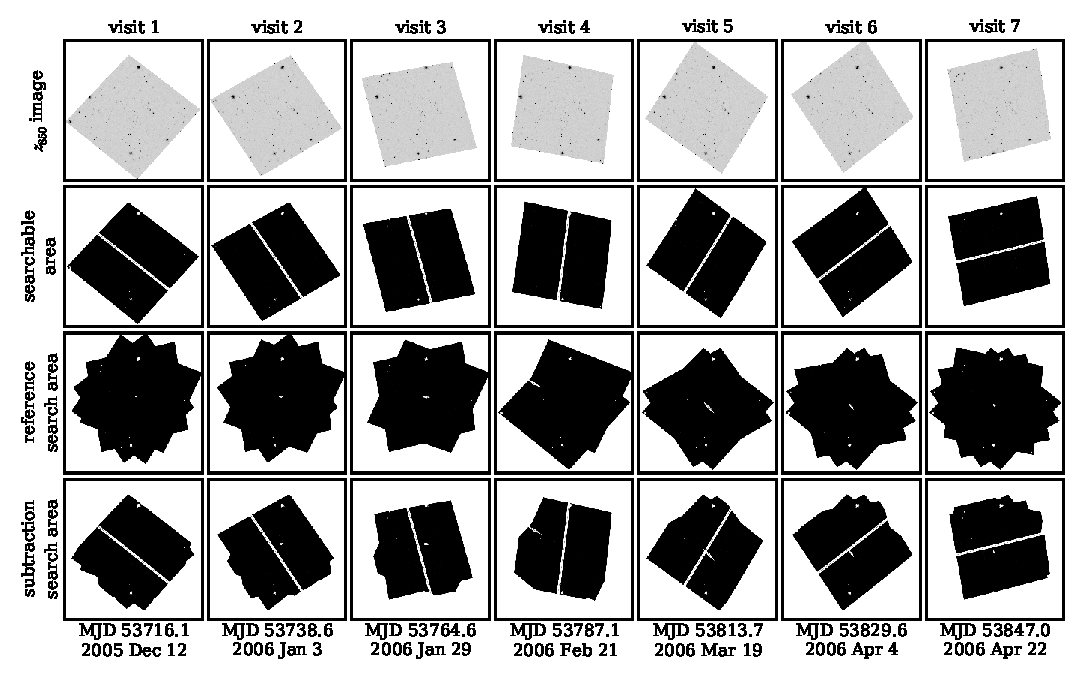
\includegraphics[width=6.75in,angle=270]{figures/cands/epochs.eps}
\end{center}
\caption[An example of image orientation and searchable regions]
{An example of image orientation and searchable regions for cluster
ISCS J1432.4+3332. Each column represents an observation of the
cluster. The first row is the $z_{850}$ image for that visit. The
second row is the part of that image that is searchable. The third row
shows the searchable area of the stacked reference image used in the
subtraction for this visit. The fourth row is the searchable area in
the subtraction (the intersection of the second and third
rows).  \label{fig:epochs}}
\end{figure}

For each ``search'' visit to each cluster, we follow these four steps:
\begin{enumerate}
\item {\bf A reference image is made} by combining images from
other visits to the cluster. All visits that are either 50 or more
days before the search epoch or 80 or more days after the search epoch
are included. If there are no epochs outside this 130~day range, the
range is narrowed symmetrically until one epoch qualifies. Masked
pixels in each visit's image do not contribute to the stacked
reference image (Fig.~\ref{fig:epochs}, third row).

\item {\bf A subtracted image is made} by subtracting the stacked
reference image from the search epoch image. A map of the sky noise
level in the subtraction is made by considering the noise level of the
search epoch image and the noise level of each reference image
contributing to a given region. Any area masked in either the search
epoch or stacked reference image is masked in the subtracted image
(Fig.~\ref{fig:epochs}, fourth row).

\item {\bf Candidates in the subtraction are identified by software.} To
  be flagged, a candidate must have three contiguous pixels with a flux
  3.4 times the local sky noise level in the subtraction (as
  determined by the sky noise map above). Once flagged, it must
  fulfill the following four requirements:
\begin{itemize}
\item {\sc MultiDrizzle}-combined image: A total signal-to-noise ratio 
  (including sky and Poisson noise) of 5 or more in a 3~pixel radius
  aperture.
\item {\sc MultiDrizzle}-combined image: A total signal-to-noise ratio 
  of 1.5 or more in a 10~pixel radius aperture.
\item Individual exposures: A signal-to-noise ratio of 1 or greater 
  in a 3~pixel radius aperture in three or more individual exposures.
\item Individual exposures: A candidate cannot have an individual exposure 
  with a flux more than $20\sigma$ greater than the flux in the lowest 
  flux exposure \emph{and} a second individual exposure with flux more 
  than $10\sigma$ greater than the flux in the lowest flux exposure.
\end{itemize}
The first requirement is designed to eliminate low significance
detections on bright galaxies. The second requirement helps eliminate
dipoles on bright galaxy cores caused by slight image misalignment. The
third and fourth requirements are aimed at false detections due to
cosmic ray coincidence. They require the candidate to be detected in
most of the exposures and allow no more than one exposure to be
greatly affected by a cosmic ray. On the order of five to ten
candidates per subtraction pass all the requirements, resulting in
approximately 1000 candidates automatically flagged across the 155
search visits.

\item {\bf Each candidate is evaluated by eye in the subtraction.}
Because the position angle changes between each epoch, the orientation
of stellar diffraction spikes changes, causing the majority of the
false detections. These are easy to detect and eliminate by
eye. Occasionally there are mis-subtractions on the cores of bright
galaxies that pass the above requirements. Only completely unambiguous
false detections are eliminated in this step. If there is any
possibility the candidate is a real SN, it is left in the sample for
further consideration.
\end{enumerate}

After carrying out the above four steps for all 155 search visit, 86
candidates remain. At this point, candidates have been selected based
only on information from a single $z_{850}$ subtraction.


\subsection{Lightcurve Requirements} \label{sec:cands_lccuts}
The 86 remaining candidates still include a considerable number of
non-SNe. We wish to trim the sample down as much as possible in an
automated way, so that we can easily calculate the efficiency of our
selection.  For each candidate, we now make three further automated
requirements based on $i_{775}$ data (if available) and the shape of
the $z_{850}$ light curve.  The requirements and number of candidates
remaining after each requirement are summarized in
Table~\ref{tab:lccuts}.

%%%%%%%%%%%%%%%%%%%%
% Light curve Cuts %
%%%%%%%%%%%%%%%%%%%%
\begin{table}[tbh]
\caption{\label{tab:lccuts} Light curve requirements for candidates}
\begin{center}
\begin{footnotesizetabular}{lc}

\hline
\hline
Requirement & Candidates Remaining \\
\hline
Before light curve requirements                   & 86\\
Positive $i_{775}$ flux (if observed in $i_{775}$) & 81\\
$2\sigma$ Detection in surrounding epochs         & 73\\
If declining, Require two $5\sigma$ detections    & 60\\
\hline

\end{footnotesizetabular}
\end{center}
\end{table}

First, we require that if $i_{775}$ data exists for the epoch in which
the candidate was detected, there be positive flux in a 2~pixel radius
aperture at the candidate location in the $i_{775}$ image. From our SN
light curve simulations, we find that virtually all SNe should pass
(near maximum light there is typically enough SN flux in the $i_{775}$
filter to result in a positive total flux, even with large negative
sky fluctuations).  Meanwhile, about half of the cosmic rays located
far from galaxies will fail this test (due to negative sky
fluctuations). If there is no $i_{775}$ data for the detection epoch,
this requirement is not applied. Even though nearly all SNe are
expected to pass, we account for any real SNe that would be removed in
our Monte Carlo simulation.

Second, we require that the light curve does not rise and fall too
quickly: if there is a ``search'' visit less than 60~days before the
detection visit and also one less than 60~days after the detection visit,
the candidate must be detected at a $2\sigma$ level in at least one of
these two visits. SNe~Ia have light curves wide enough to be detected
at this level in two epochs spaced apart by 60~days. However, cosmic
rays in one $z_{850}$ image are unlikely to be repeated in the same
spot in two epochs and thus will be removed. This requirement is also
included in our Monte Carlo simulation.

%The third and final requirement eliminates SNe lacking
%sufficient light curve information for typing. 
%Because we cannot
%obtain spectroscopic confirmation for all candidates, it is important
%to have enough light curve information to be able the estimate a SN
%type photometrically. 
The third and final requirement aims to eliminate candidates that were
significantly detected in only the first epoch and that then faded
from view. Such candidates would not have been followed up
spectroscopically and it would typically be impossible to tell if such
candidates were SNe (and if so, Type~Ia or core collapse) on the basis
of a single detection. We chose to eliminate any such candidates and
account for this elimination in our Monte Carlo simulation, rather
than dealing with an ``untypeable'' candidate.  Specifically, if a
candidate is found on the decline (in the first search epoch), we
require two epochs with $5\sigma$ detections.  For high-redshift
($z \sim 1$) SNe~Ia, this requirement means that the first epoch will
be at approximately maximum light, and most of the SN decline is
captured, making it possible to confirm a SN and estimate a type.
For candidates that are only significantly detected in the last search
epoch, typing is not a problem because additional ACS orbits were
typically scheduled in order to follow such candidates.

After these requirements 60 candidates remain. The automatic selection
means that we can easily calculate the completeness of the selection
so far; any real SNe~Ia removed will be accounted for in the
``effective visibility time'' which is calculated using a
Monte Carlo simulation.


\section{Type Determination} \label{sec:cands_typing}

We now use all available information about each candidate
(spectroscopic confirmation, host galaxy redshift, all light curve
information, as well as host galaxy luminosity and color) to classify
each of the 60 remaining candidates as image artifact, active galactic
nucleus (AGN), core-collapse SN (SN~CC), or SN~Ia.
%Because the amount of information varies greatly among candidates,
%we must consider each candidate on an individual basis, meaning that a
%selection efficiency cannot be automatically computed. Instead, we
%estimate a systematic error in the final result from possible
%mis-classifications in this step. 
%Note that although not every candidate is discussed individually here,
%all 60 candidates can be viewed in detail
%at \url{http://supernova.lbl.gov/cands/cands.html}.

%We will show that for nearly all candidates classified as AGN or image
%artifacts, we can say with certainty that they are \emph{not} SNe~Ia
%on the basis of the complete light curve and limits on host galaxy
%redshifts.  We will also show that most of the remaining candidates
%can be unambiguously classified as SNe~Ia or SNe II. 


\subsection{Image Artifacts} \label{sec:cands_artifacts}
 
%%%%%%%%%%%%%%%%%%%%%%%%%%%%%%%%%%%%%%%%%%%%%%%%%%%%%%%%%%%%%%%%%%%%%%%%%%
% Artifacts candidates figure                                            %
%%%%%%%%%%%%%%%%%%%%%%%%%%%%%%%%%%%%%%%%%%%%%%%%%%%%%%%%%%%%%%%%%%%%%%%%%%

\begin{figure}[!b]
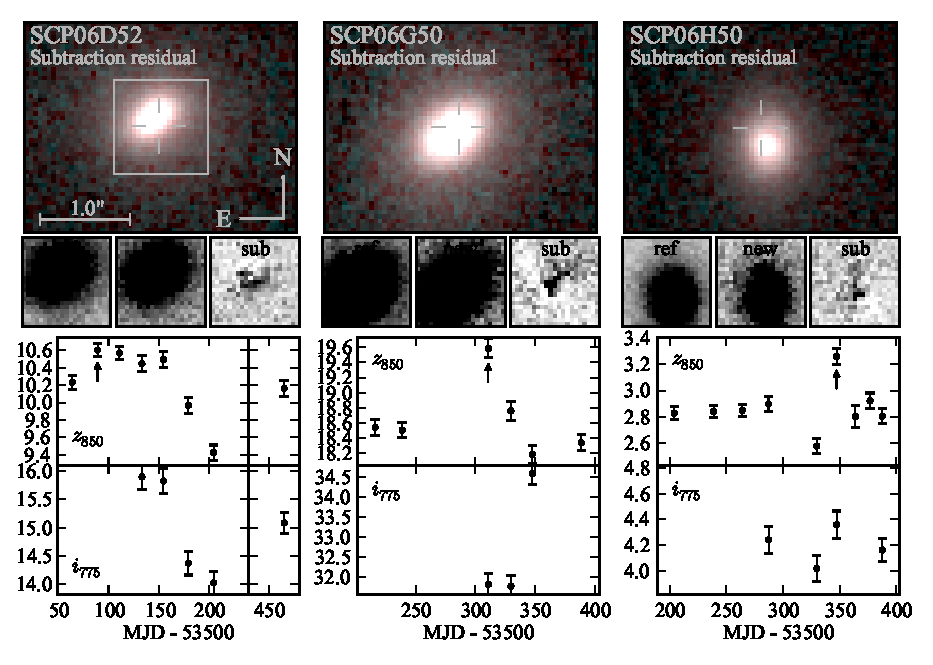
\includegraphics[width=\textwidth]{figures/cands/artifacts1.eps}
\caption[Images and light curves of candidates classified as artifacts]
        {Images and light curves of the candidates classified as image
         artifacts (cosmic ray hits and/or subtraction residuals). For
         each candidate, the \emph{top panel} shows the two-color
         stacked image ($i_{775}$ and $z_{850}$) of the host galaxy,
         with the position of the transient indicated.  The \emph{three
         smaller panels} below the stacked image show the reference,
         new, and subtracted images for the discovery visit. The \emph{bottom
         panel} shows the light curve at the transient position (including
         host galaxy light) in the $z_{850}$ ({\it top}) and $i_{775}$
         ({\it bottom}) bands. The y axes have units of counts per
         second in a $3$~pixel radius aperture. The effective
         zeropoints are 23.94 and 25.02 for $z_{850}$ and $i_{775}$,
         respectively. The discovery visit is indicated with an arrow
         in the $z_{850}$ plot. [\emph{Continued on next three pages.}]
         \label{fig:artifacts}}
\end{figure}

\begin{figure}[p]
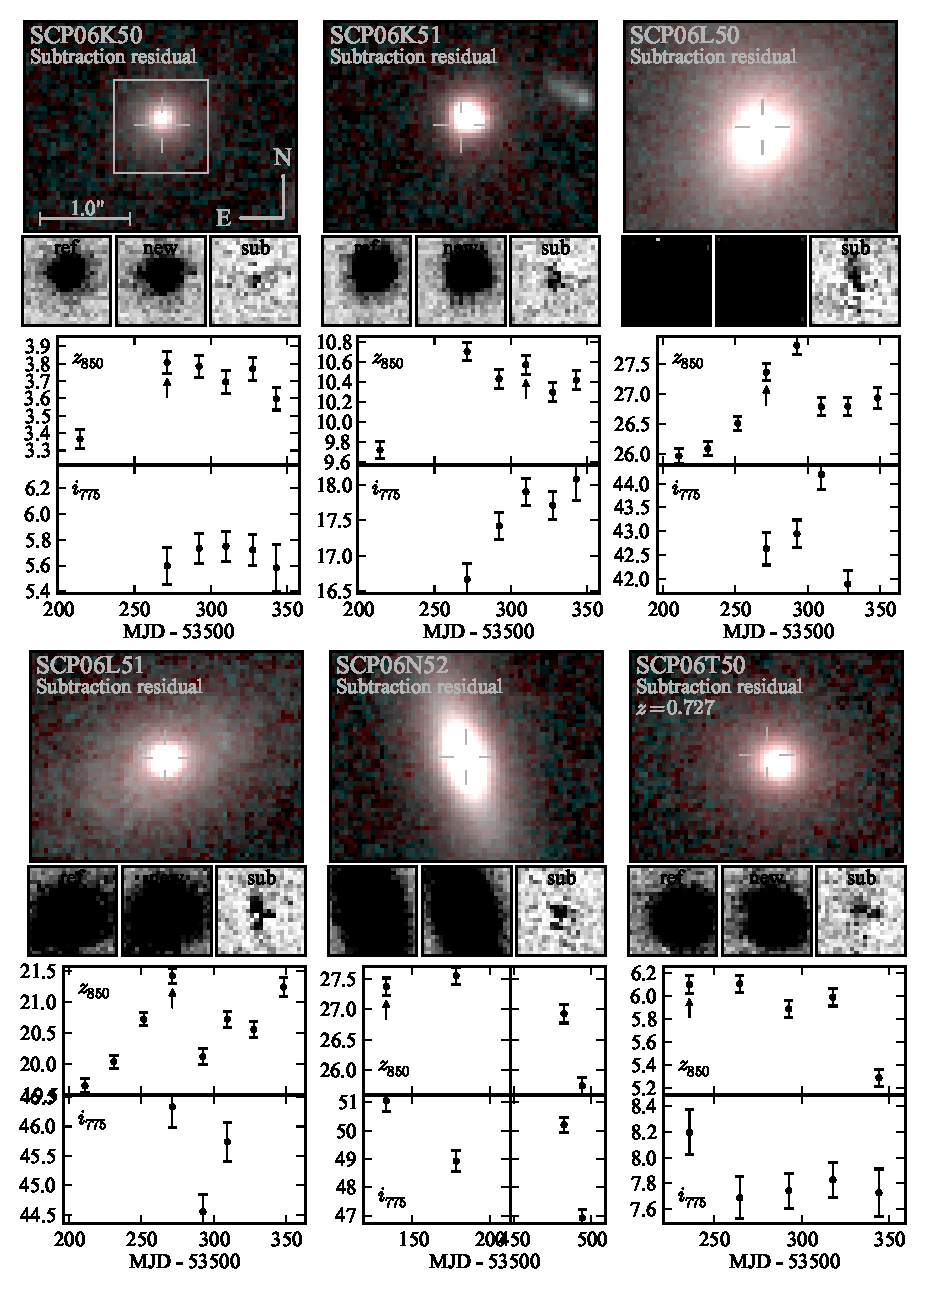
\includegraphics[width=\textwidth]{figures/cands/artifacts2.eps}
\end{figure}

\begin{figure}[p]
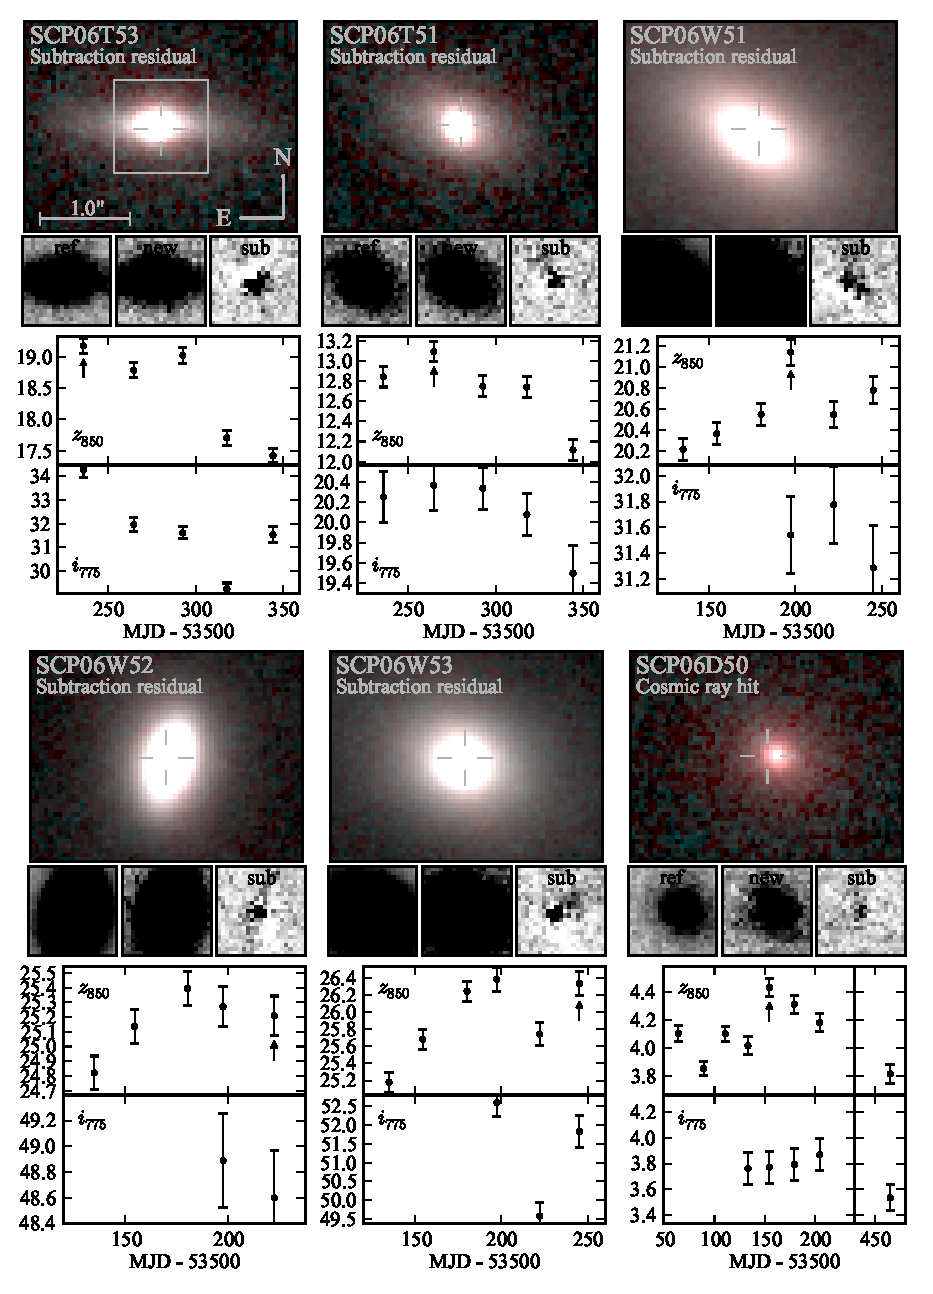
\includegraphics[width=\textwidth]{figures/cands/artifacts3.eps}
\end{figure}

\begin{figure}[t]
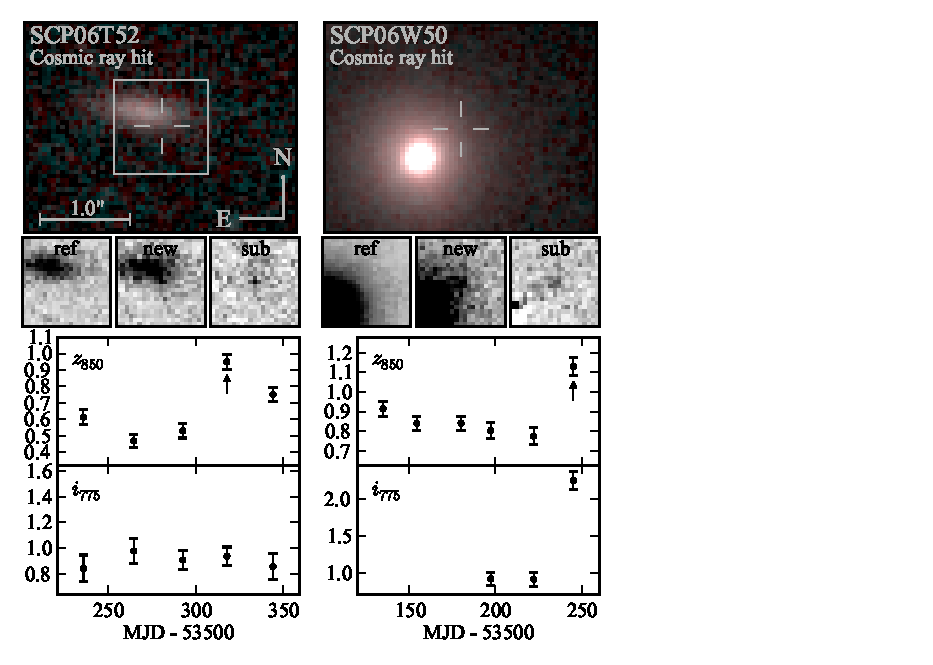
\includegraphics[width=\textwidth]{figures/cands/artifacts4.eps}
\end{figure}

Although the automated selections were designed to eliminate image
artifacts such as subtraction residuals and cosmic rays, they were
made to be somewhat tolerant so that real SNe were not eliminated. The
result is that some artifacts slip through. Candidates located close
to the cores of relatively bright galaxies that show adjoining
negative and positive areas in subtractions are likely to be caused by
mis-alignment between the reference and search image. For such
candidates, we inspected the full light curve for consistency with the
general shape of a SN~Ia light curve. For fourteen of these, the
light curve is completely inconsistent with that of a SN~Ia. Their
light curves have either multiple peaks, long flat portions followed
by one or two lower points, and/or $i_{775}$ data that shows no
change. We classify these fourteen candidates as subtraction residuals
with negligible classification uncertainty (very unlikely that any are
SNe~Ia). These candidates are shown in Figure~\ref{fig:artifacts}.
%Additionally, the peak-to-peak change in $z_{850}$ flux is
%typically too small to be compatible with a SN~Ia, given that the
%galaxies are generally too bright and too blue to be at high
%redshift. For example, seven candidates are on galaxies of $z_{850} <
%20$), yet show peak-to-peak magnitude changes of only $z_{850} \gtrsim
%23.3$, too dim for a SN~Ia at such redshifts.

Candidates where one or two of the four $z_{850}$ exposures was
clearly affected by a cosmic ray or hot pixel may be false
detections. These can pass the automated cosmic ray rejection when
they occur on a galaxy.  For two such candidates, we used the lack of
any change in the $i_{775}$ light curve to rule out a SN~Ia: fitting
SN templates with a range of redshifts and extinctions resulted in
observed $i_{775}$ fluxes too low by $4\sigma$ or more, given the
$z_{850}$ increase. One other candidate, SCP06W50, is less certain. It
was discovered in the last visit to the cluster, making it difficult
to constrain a template light curve. There is clearly a hot pixel or
cosmic ray in one $z_{850}$ exposure, but there appears to be some
excess flux in the other three exposures as well. Also, there is a
point-source like detection in $i_{775}$, but offset $\sim$1.2~pixels
from the $z_{850}$ detection. While the $i_{775}$ detection may also
be a cosmic ray, it is possible that this candidate is a SN caught
very early. The elliptical ``host'' galaxy was not observed
spectroscopically, but we estimate its redshift to be $0.60 < z < 0.85$
based on the color of $i_{775} - z_{850} = 0.55$ and stellar
population models of \citet[][hereafter BC03]{bruzual03a}.

Of the 17 total candidates classified as image artifacts, SCP06W50 is the
only one with significant uncertainty. However, this uncertainty does
not affect the cluster SN~Ia rate as the host galaxy is clearly in the
cluster foreground.


\subsection{AGN} \label{sec:cands_agn}

%%%%%%%%%%%%%%%%%%%%%%%%%%%%%%%%%%%%%%%%%%%%%%%%%%%%%%%%%%%%%%%%%%%%%%%%%%
% AGN candidates figure                                                  %
%%%%%%%%%%%%%%%%%%%%%%%%%%%%%%%%%%%%%%%%%%%%%%%%%%%%%%%%%%%%%%%%%%%%%%%%%%

\begin{figure}[!b]
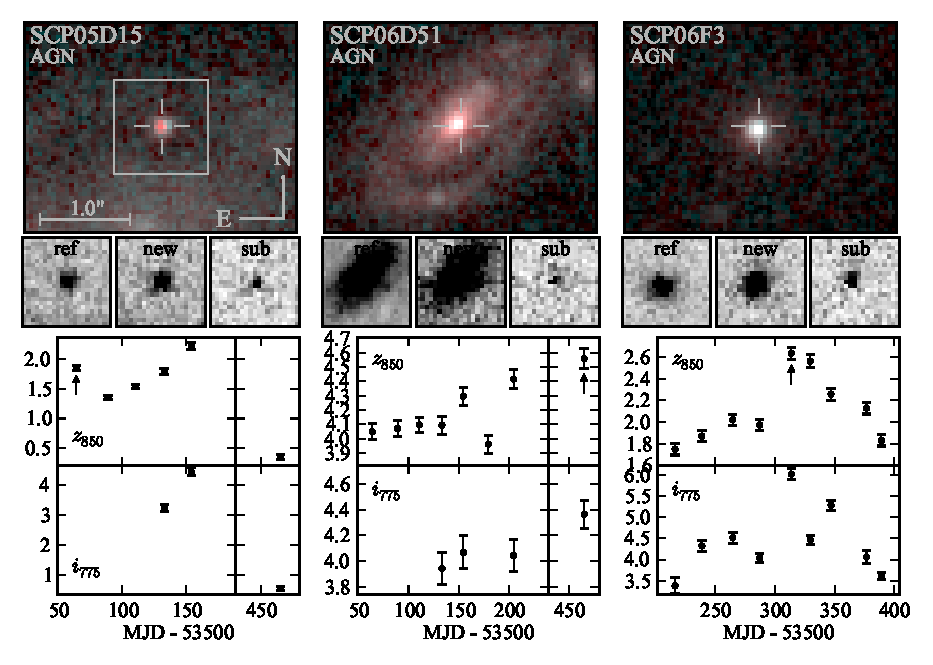
\includegraphics[width=\textwidth]{figures/cands/agn1.eps}
\caption[Images and light curves of candidates classified as AGN]
        {Images and light curves of the candidates classified as
          AGN. For each candidate, the \emph{top panel} shows the
          two-color stacked image ($i_{775}$ and $z_{850}$) of the
          host galaxy, with the position of the transient indicated.
          The \emph{three smaller panels} below the stacked image show the
          reference, new, and subtracted images for the discovery
          visit. The \emph{bottom panel} shows the light curve at the transient
          position (including host galaxy light) in the $z_{850}$
          ({\it top}) and $i_{775}$ ({\it bottom}) bands. The y axes
          have units of counts per second in a $3$~pixel radius
          aperture. The effective zeropoints are 23.94 and 25.02 for
          $z_{850}$ and $i_{775}$, respectively. The discovery visit
          is indicated with an arrow in the $z_{850}$
          plot. [\emph{Continued on next two pages.}]\label{fig:agn}}
\end{figure}

\begin{figure}[p]
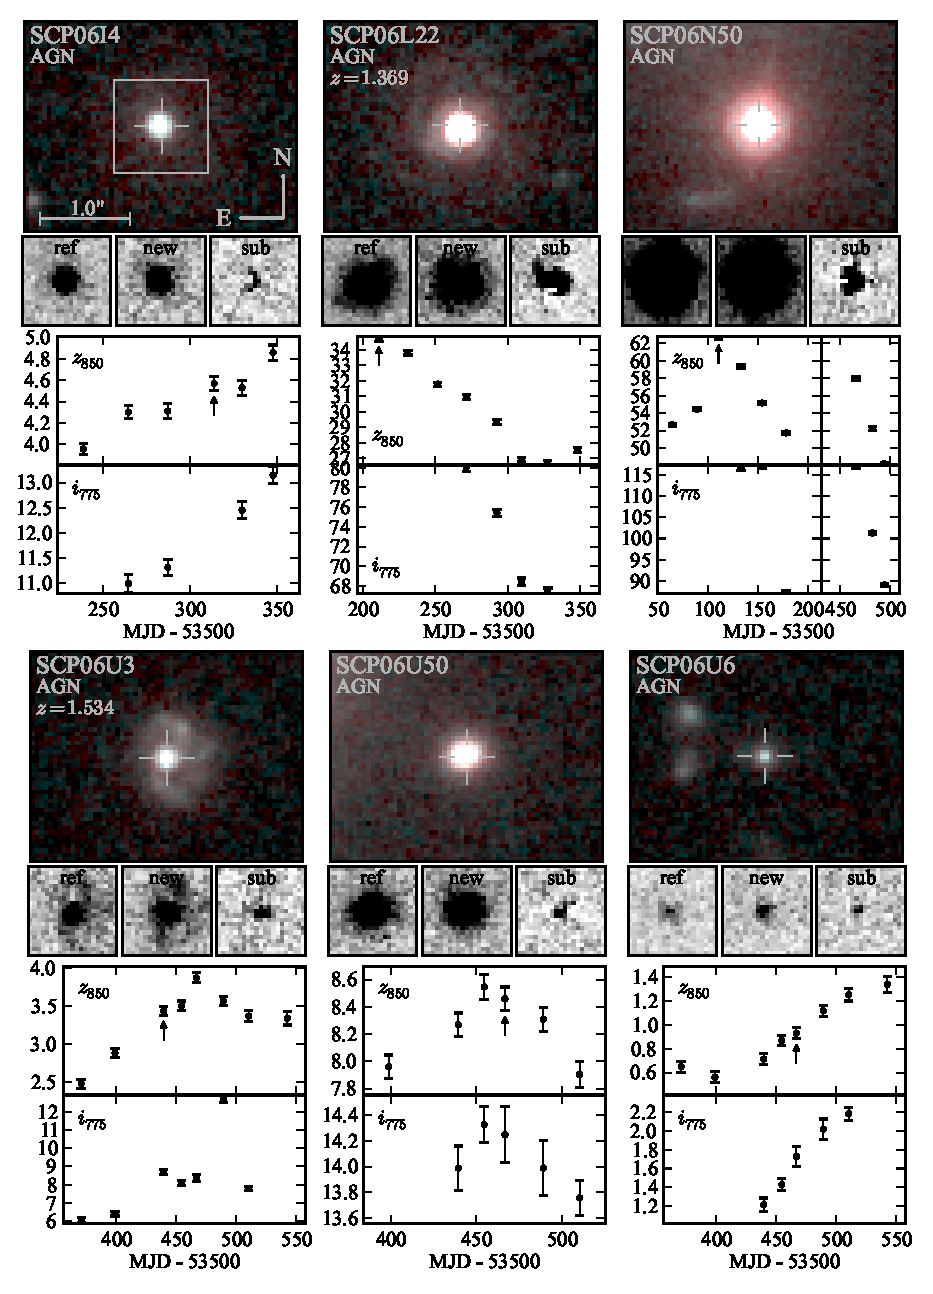
\includegraphics[width=\textwidth]{figures/cands/agn2.eps}
\end{figure}

\begin{figure}[p]
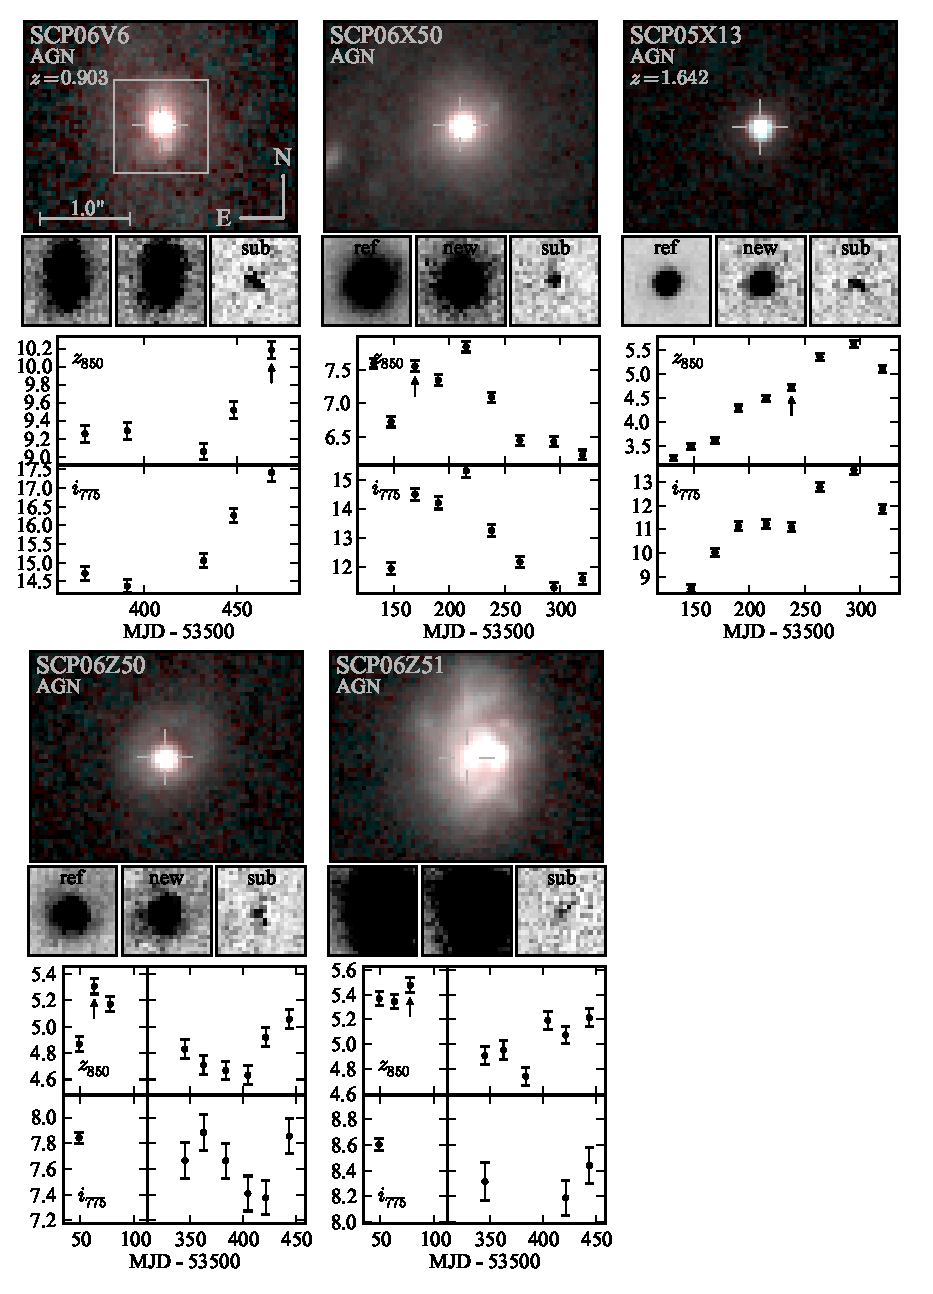
\includegraphics[width=\textwidth]{figures/cands/agn3.eps}
\end{figure}

Candidates positioned directly on the cores of their host galaxies may
be AGN. Four such candidates were spectroscopically confirmed as AGN:
SCP06L22 ($z=1.369$), SCP06V6 ($z=0.903$) and SCP05X13 ($z=1.642$) and
SCP06U3 ($z=1.534$). A fifth candidate, SCP06F3, is spectroscopically
consistent with an AGN at $z=1.21$, but is less certain \citep[see
  spectroscopy reported in][]{morokuma10a}. SCP06L22, SCP05X13,
SCP06U3 and SCP06F3 also have light curves that are clearly
inconsistent with SNe~Ia (observer frame rise times of 100~days or
more, or declining phases preceding rising phases; see
Fig.~\ref{fig:agn}). Of the ``on core'' candidates that were not
observed spectroscopically, five exhibit light curves that decline
before rising or have rise times of 100~days or more. A sixth
candidate, SCP06Z51 exhibited slightly varying fluxes that could be
due to either subtraction residuals or an AGN.  However, its light
curve is clearly inconsistent with a SN~Ia, especially considering the
apparent size, magnitude and color of the host galaxy. Summarizing,
there are 11 ``on-core'' candidates certain not to be SNe~Ia.

Three other ``on-core'' candidates are also considered likely AGN on
the basis of their light curves: SCP06Z50, SCP06U50 and
SCP06D51. SCP06Z50 has a rise-fall behavior in the first three
$z_{850}$ observations of its light curve that \emph{could} be
consistent with a SN~Ia light curve. However, given that the host
galaxy is likely at $z \lesssim 1$ based on its magnitude and color,
the SN would be fainter than a normal SN~Ia by 1~magnitude or
more. Considering the proximity to the galaxy core and the additional
variability seen in the last two observations, SCP06Z50 is most likely
an AGN. The light curve of candidate SCP06U50 also exhibits a
rise-fall that could be consistent with a supernova light
curve. However, its host is morphologically elliptical and likely at
$z \lesssim 0.7$ based on its color. At $z \lesssim 0.7$, a SN~Ia
would have to be very reddened ($E(B-V) \gtrsim 1$) to match the color
and magnitude of the SCP06U50 light curve. As this is very unlikely
(considering that the elliptical host likely contains little dust), we
conclude that SCP06U50 is also most likely an AGN. Finally, SCP06D51
was discovered in the last visit, on the core of a spiral galaxy. We
classify it as an AGN based on the earlier variability in the light
curve. As these galaxies are all most likely in the cluster
foregrounds, even the small uncertainty in these classifications is
not a concern for the cluster rate calculation here.

Note that one of the candidates classified here as a clear AGN,
SCP06U6, was reported as a SN with unknown redshift by
\citet{dawson09a}, due to the fact that spectroscopy revealed no
evidence of an AGN.  However, it is on the core of a compact galaxy,
and has a clear $\gtrsim 100$ day rise in both $z_{850}$ and
$i_{775}$. While it could possibly be a very peculiar SN with a long
rise time, what is important for this analysis is that it is clearly
not a SN~Ia.



\subsection{Supernovae} \label{sec:cands_sn}

%%%%%%%%%%%%%%%%%%%%%%%
% SN candidates table %
%%%%%%%%%%%%%%%%%%%%%%%

\begin{table}[p]
\caption{\label{tab:sn} Candidates classified as supernovae}
\begin{center}
\begin{footnotesizetabular}{lccccccc}

\hline
\hline
ID & Nickname & R.A. (J2000) & Decl. (J2000) & $z$ & Type & Conf. & How? \\
\hline
\multicolumn{8}{l}{\emph{Cluster Members}} \\
SCP06C1 & Midge & $12^{\rm h}\,29^{\rm m}\,33^{\rm s}.012$ & $+01^{\circ}\,51'\,36''.67$ & 0.98\phn & Ia & secure & a,c\\
SCP05D0 & Frida & $02^{\rm h}\,21^{\rm m}\,42^{\rm s}.066$ & $-03^{\circ}\,21'\,53''.12$ & 1.014 & Ia & secure & a,b,c\\
SCP06F12 & Caleb & $14^{\rm h}\,32^{\rm m}\,28^{\rm s}.748$ & $+33^{\circ}\,32'\,10''.05$ & 1.11\phn & Ia & probable & c\\
SCP06H5 & Emma & $14^{\rm h}\,34^{\rm m}\,30^{\rm s}.139$ & $+34^{\circ}\,26'\,57''.29$ & 1.231 & Ia & secure & b,c\\
SCP06K18 & Alexander & $14^{\rm h}\,38^{\rm m}\,10^{\rm s}.663$ & $+34^{\circ}\,12'\,47''.19$ & 1.412 & Ia & probable & b\\
SCP06K0 & Tomo & $14^{\rm h}\,38^{\rm m}\,08^{\rm s}.366$ & $+34^{\circ}\,14'\,18''.08$ & 1.416 & Ia & secure & b,c\\
SCP06R12 & Jennie & $02^{\rm h}\,23^{\rm m}\,00^{\rm s}.082$ & $-04^{\circ}\,36'\,03''.04$ & 1.212 & Ia & secure & b,c\\
SCP06U4 & Julia & $23^{\rm h}\,45^{\rm m}\,29^{\rm s}.429$ & $-36^{\circ}\,32'\,45''.73$ & 1.05\phn & Ia & secure & a,c\\
\multicolumn{8}{l}{\emph{Cluster Membership Uncertain}} \\
SCP06E12 & Ashley & $14^{\rm h}\,15^{\rm m}\,08^{\rm s}.141$ & $+36^{\circ}\,12'\,42''.94$ & \nodata & Ia & plausible & c\\
SCP06N32 & \nodata & $02^{\rm h}\,20^{\rm m}\,52^{\rm s}.368$ & $-03^{\circ}\,34'\,13''.32$ & \nodata & CC & plausible & c\\
\multicolumn{8}{l}{\emph{Not Cluster Members}} \\
SCP06A4 & Aki & $22^{\rm h}\,16^{\rm m}\,01^{\rm s}.077$ & $-17^{\circ}\,37'\,22''.09$ & 1.193 & Ia & probable & c\\
SCP06B3 & Isabella & $22^{\rm h}\,05^{\rm m}\,50^{\rm s}.402$ & $-01^{\circ}\,59'\,13''.34$ & 0.743 & CC & probable & c\\
SCP06C0 & Noa & $12^{\rm h}\,29^{\rm m}\,25^{\rm s}.654$ & $+01^{\circ}\,50'\,56''.58$ & 1.092 & Ia & secure & b,c\\
SCP06C7 & \nodata & $12^{\rm h}\,29^{\rm m}\,36^{\rm s}.517$ & $+01^{\circ}\,52'\,31''.47$ & 0.61\phn & CC & probable & c\\
SCP05D6 & Maggie & $02^{\rm h}\,21^{\rm m}\,46^{\rm s}.484$ & $-03^{\circ}\,22'\,56''.18$ & 1.314 & Ia & secure & b,c\\
SCP06F6 & \nodata & $14^{\rm h}\,32^{\rm m}\,27^{\rm s}.394$ & $+33^{\circ}\,32'\,24''.83$ & 1.189 & non-Ia & secure & a\\
SCP06F8 & Ayako & $14^{\rm h}\,32^{\rm m}\,24^{\rm s}.525$ & $+33^{\circ}\,33'\,50''.75$ & 0.789 & CC & probable & c\\
SCP06G3 & Brian & $14^{\rm h}\,29^{\rm m}\,28^{\rm s}.430$ & $+34^{\circ}\,37'\,23''.13$ & 0.962 & Ia & plausible & c\\
SCP06G4 & Shaya & $14^{\rm h}\,29^{\rm m}\,18^{\rm s}.743$ & $+34^{\circ}\,38'\,37''.38$ & 1.35\phn & Ia & secure & a,b,c\\
SCP06H3 & Elizabeth & $14^{\rm h}\,34^{\rm m}\,28^{\rm s}.879$ & $+34^{\circ}\,27'\,26''.61$ & 0.85\phn & Ia & secure & a,c\\
SCP06L21 & \nodata & $14^{\rm h}\,33^{\rm m}\,58^{\rm s}.990$ & $+33^{\circ}\,25'\,04''.21$ & \nodata & CC & plausible & c\\
SCP06M50 & \nodata & $16^{\rm h}\,04^{\rm m}\,25^{\rm s}.300$ & $+43^{\circ}\,04'\,51''.85$ & \nodata & \nodata & \nodata & \nodata\\
SCP05N10 & Tobias & $02^{\rm h}\,20^{\rm m}\,52^{\rm s}.878$ & $-03^{\circ}\,33'\,40''.20$ & 0.203 & CC & plausible & c\\
SCP06N33 & Naima & $02^{\rm h}\,20^{\rm m}\,57^{\rm s}.699$ & $-03^{\circ}\,33'\,23''.97$ & 1.188 & Ia & probable & c\\
SCP05P1 & Gabe & $03^{\rm h}\,37^{\rm m}\,50^{\rm s}.352$ & $-28^{\circ}\,43'\,02''.66$ & 0.926 & Ia & probable & c\\
SCP05P9 & Lauren & $03^{\rm h}\,37^{\rm m}\,44^{\rm s}.512$ & $-28^{\circ}\,43'\,54''.58$ & 0.821 & Ia & secure & a,c\\
SCP06U7 & Ingvar & $23^{\rm h}\,45^{\rm m}\,33^{\rm s}.867$ & $-36^{\circ}\,32'\,43''.48$ & 0.892 & CC & probable & c\\
SCP06X26 & Joe & $09^{\rm h}\,10^{\rm m}\,37^{\rm s}.889$ & $+54^{\circ}\,22'\,29''.07$ & 1.44\phn & Ia & plausible & c\\
SCP06Z5 & Adrian & $22^{\rm h}\,35^{\rm m}\,24^{\rm s}.966$ & $-25^{\circ}\,57'\,09''.61$ & 0.623 & Ia & secure & a,c \\
\hline
\end{footnotesizetabular}

\end{center}
{\footnotesize {\bf Note.} --- ``How?'' indicates how the type is
  determined.  (a) Spectroscopic confirmation.  (b) Host is
  morphologically early-type, with no signs of recent star formation.
  (c) Light curve shape, color, magnitude consistent with type. We do
  not assign a type for SCP06M50 because there is significant
  uncertainty that the candidate is a SN at all.}
\end{table}

After removing 17 image artifacts and 14 AGN, 29 candidates remain
(listed in Table~\ref{tab:sn}). One of these is the peculiar
transient SN~SCP06F6 which, as noted above, is clearly not a SN~Ia.
Note that Table~\ref{tab:sn} contains 10 fewer candidates than the
list presented by \citet{dawson09a}. This is unsurprising; here we have
intentionally used a stricter selection than in the original search,
the source for the \citet{dawson09a} sample. Still, after finalizing our
selection method we checked that there were no unexpected
discrepancies. Five of the \citet{dawson09a} candidates (SCP06B4, SCP06U2,
SCP06X18, SCP06Q31, SCP06T1) fell just below either the detection or
signal-to-noise thresholds in our selection. These were found in the
original search because detection thresholds were set slightly lower,
and because the images were sometimes searched in several different
ways. For example, in the original search SCP06B4 was only found by
searching an $i_{775}$ subtraction. Two \citet{dawson09a} candidates (SCP05D55,
SCP06Z52) were found too far on the decline and failed the light curve
requirements (\S\ref{sec:cands_lccuts}). Three \citet{dawson09a} candidates (SCP06X27,
SCP06Z13, SCP06Z53) were found while searching in ``follow-up''
visits, which were not searched here. SCP06U6 passed all requirements,
but is classified here as an AGN, as noted above. With the exception
of SCP06U6, all of these candidates are likely to be supernovae
(mostly core collapse). However, the types of candidates that did not
pass our requirements are not of concern for this analysis. Finally,
SCP06M50 was not reported in \citet{dawson09a}, but is classified here as a SN,
although with great uncertainty (discussed in detail
in \S\ref{sec:cands_sncomments}).

Thanks to the extensive ground-based spectroscopic follow-up campaign,
we were able to obtain spectroscopic redshifts for 25 of the 29
SNe. The redshift reported in Table~\ref{tab:sn} is derived from the
SN host galaxy for all but one candidate (SCP06C1) where the redshift
is from the SN spectrum itself. Of the 25 candidates with redshifts,
eight are in clusters and 17 are in the field. Note that this high
spectroscopic completeness is particularly important for determining
the cluster or non-cluster status of each SN, which directly affects
the determination of the cluster SN~Ia rate. The possible cluster
memberships of the four candidates lacking redshifts are discussed
below.

We determine the type of each of the 29 supernovae using a combination
of methods in order to take into account all available information for
each supernova. This includes (a) spectroscopic confirmation, (b) the
host galaxy environment, and (c) the SN light curve. To qualify the
confidence of each supernova's type, we rank the type as ``secure,''
``probable,'' or ``plausible'':
\begin{description}
\item[Secure SN~Ia] Has
spectroscopic confirmation or \emph{both} of the following: (1) an
early-type host galaxy with no recent star formation and (2) a light
curve with shape, color and magnitude consistent with SNe~Ia and
inconsistent with other types.
\item[Probable SN~Ia] Fulfills either the host galaxy 
requirement or the light curve requirement, but not both.
\item[Plausible SN~Ia] The light curve is indicative of a SN~Ia, 
but there is not enough data to rule out other types.
\item[Secure SN~CC] Has spectroscopic confirmation (note that 
there are no such candidates in this sample). 
\item[Probable SN~CC] The light curve is consistent with a 
core-collapse SN and inconsistent with a SN~Ia. 
\item[Plausible SN~CC] Has a light curve indicative
of a core-collapse SN, but not inconsistent with a SN~Ia. 
\end{description}
This ranking system is largely comparable to the ``gold,'' ``silver,''
``bronze'' ranking system of \citet{strolger04a}, except that we do
not use their ``UV deficit'' criterion. This is because our data do
not include the bluer F606W filter, and because SNe~Ia and CC are
only distinct in UV flux for a relatively small window early in the
light curve. Below, we discuss in detail the three typing methods used.

%Obtaining spectroscopic
%confirmation of SNe at $z \gtrsim 1$ remains notoriously difficult,
%whether from the ground or from space. In a high-redshift SN rate
%study, one cannot hope to obtain a spectroscopic type for \emph{every}
%SN candidate. Therefore, we rely on the properties of the host galaxy
%and the light curve of the SN in typing the majority of the
%supernovae.

{\bf (a) Spectroscopic confirmation:} During the survey, seven
candidates were spectroscopically confirmed as
SNe~Ia \citep{dawson09a,morokuma10a}. These seven (three of which are in
clusters) are designated with an ``a'' in the ``typing'' column of
Table~\ref{tab:sn}. All seven candidates have a light curve shape,
absolute magnitude and color consistent with a SN~Ia. Although the
spectroscopic typing by itself has some degree of uncertainty, the
corroborating evidence from the light curve makes these ``secure''
SNe~Ia.

{\bf (b) Early-type host galaxy:} The progenitors of core-collapse SNe
are massive stars ($> 8 M_{\odot}$) with main sequence lifetimes of
$<40$~Myr. Thus, core-collapse SNe only occur in galaxies with recent
star formation. Early-type galaxies, having typically long ceased star
formation, overwhelmingly host Type~Ia
SNe \citep[e.g.,][]{cappellaro99a,hamuy00a}. In fact, in an extensive
literature survey of core-collapse SNe reported in early-type
hosts, \citet{hakobyan08a} found that only three core-collapse SNe
have been recorded in early-type hosts, and that the three host
galaxies in question had either undergone a recent merger or were
actively interacting. In all three cases there are independent
indicators of recent star formation. Therefore, in the cases where the
host galaxy morphology, photometric color, and spectrum all indicate
an early-type galaxy with no signs of recent star formation or
interaction, we can be extremely confident that the SN type is
Ia. These cases are designated by a ``b'' in the ``typing'' column of
Table~\ref{tab:sn}. We emphasize that in all of these cases,
spectroscopy reveals no signs of recent star formation and there are
no visual or morphological signs of interaction. \citep[See][for
detailed studies of these SN host galaxy properties.]{meyers11a}

%In Meyers11 we quantify the upper limit on any core-collapse SNe that
%might come from recent star formation in each of these host
%galaxies. We use the upper limit on the spectroscopic [OII] flux to
%place a limit on recent star formation.  In each case, the upper limit
%on the rate of SNe~CC is a factor of at least several lower than the
%expected SN~Ia rate. Note that these are limits on the expected ratio
%of the \emph{intrinsic} rates. The expected ratio of
%\emph{observed} rates will be even larger, due to the fact that at these high
%redshifts we would not detect most SNe~CC even if they did occur in
%these galaxies, while the large majority of SNe~Ia are detectable.

%In all but one of these cases (SCP06K18) we also have
%a full light curve in two bands consistent with a SN~Ia, further
%increasing our confidence in the type.

%The exception,
%SCP06K18, has only two observations during the active phase of the
%light curve (see Fig.~\ref{fig:sn}) and is somewhat less certain. We
%give it a ``probable'' rank to reflect the possibility that there is
%some low level of star formation not detected in the host
%spectrum. However, this is still a very likely SN~Ia, particularly
%considering that the upper limit on the star formation rate is very
%low and that only a small fraction of SNe~CC are as luminous as
%SCP06K18. (For example, \citet{li10a} find {\it no} SNe~CC this
%bright).

{\bf (c) Light curve:} SNe~Ia can be distinguished from most common
types of SNe~CC by some combination of light curve shape, color, and
absolute magnitude.  We compare the light curve of each candidate to
template light curves for SN~Ia and various SN~CC subtypes to test if
the candidate could be a SN~Ia or a SN~CC. For candidates lacking
both spectroscopic confirmation and an elliptical host galaxy, if
there is sufficient light curve data to rule out all SN~CC subtypes,
the candidate is considered a ``probable'' SN~Ia. If SN~Ia can be
ruled out, it is considered a ``probable'' SN~CC. If neither SN~Ia nor
SN~CC can be ruled out, the candidate is considered a ``plausible''
SN~Ia or SN~CC based on how typical the candidate's absolute magnitude
and/or color would be of each type. This approach can be viewed as a
qualitative version of the pseudo-Bayesian light curve typing
approaches of,
e.g., \citet{kuznetsova07a,kuznetsova08a,poznanski07b,poznanski07a}. SNe
classified as ``probable'' here would likely have a Bayesian posterior
probability approaching $1$, while ``plausible'' SNe would have an
intermediate probability (likely between 0.5 and 1.0). We consciously
avoid the full Bayesian typing approach because it can obscure large
uncertainties in the priors such as luminosity distributions, relative
rates, light curve shapes, and SN subtype fractions. Also, the
majority of our candidates have more available light curve information
than those of \citet{kuznetsova08a} and \citet{poznanski07a}, making a
calculation of precise classification uncertainty less necessary. In
general, classification uncertainty from light curve fitting is not a
concern for the cluster rate calculation as most cluster-member
candidates are securely typed using methods (a) and/or (b), above.

For each candidate we fit template light curves for SN~Ia, Ibc, II-P,
II-L, and IIn. We use absolute magnitude and color as a discriminant
by limiting the allowed fit ranges according to the known
distributions for each subtype. For SN~Ia we start with the spectral
time series template of \citet{hsiao07a}, while for the core-collapse
types we use templates
of \citet{nugent02a}\footnote{See \url{http://supernova.lbl.gov/~nugent/nugent_templates.html}.}.
Each spectral time series is redshifted to the candidate redshift and
warped according to the desired color. Observer-frame template light
curves are then generated by synthetic photometry in the $i_{775}$ and
$z_{850}$ filters. The magnitude, color, date of maximum light, and
galaxy flux in $i_{775}$ and $z_{850}$ are allowed to vary to fit the
light curve data. For the SN~Ia template, the linear timescale or
``stretch'' \citep[e.g.,][]{perlmutter97a,guy05a} is also allowed to
vary within the range $0.6 < s < 1.3$.  We constrain the absolute
magnitude for each subtype to the range observed by \citet{li10a}; Our
allowed range fully encompasses their observed luminosity functions
(uncorrected for extinction) for a magnitude-limited survey for each
subtype. We correct from their assumed value of $H_0 =
73$~km~s$^{-1}$~Mpc$^{-1}$ to our assumed value of $H_0 =
70$~km~s$^{-1}$~Mpc$^{-1}$ and $K$-correct from $R$ to $B$ band. To
avoid placing too strict of an upper limit on SN~CC brightness, we use
the bluest maximum-light spectrum available when $K$-correcting (e.g.,
for SN Ibc we use a bluer spectrum than that of \citet{nugent02a}, as
bluer SNe Ibc have been observed). The resulting allowed $M_B$ range
for each subtype is shown in Table~\ref{tab:snfit}. Note that the
range for Ibc does not include ultra-luminous SNe~Ic (such as those in
the luminosity functions of \citet{richardson02a}) as none were
discovered by \citet{li10a}. While such SNe can mimic a SN~Ia
photometrically, the \citet{li10a} results indicate that they are
intrinsically rare, and even \citet{richardson02a} show that they make
up at most $\sim$20\% of all SNe~Ibc. Still, we keep in mind that even
candidates compatible only with our SN~Ia template and incompatible
with SN~CC templates may in fact be ultra-luminous SNe~Ic, though the
probability is low. This is why any candidate typed based on light
curve alone has a confidence of at most ``probable,'' rather than
``secure.''  The allowed ranges of ``extinction,'' $E(B-V)$, are also
shown in Table~\ref{tab:snfit}. For SN~Ia, $E(B-V)$ is the
difference in $B-V$ color from the \citet{hsiao07a} template. As the
observed distribution of SNe includes SNe
bluer than this template, SNe~Ia as blue as $E(B-V) = -0.2$ are
allowed. Given an $E(B-V)$, the spectral template is warped according
to the {\sc salt} color law \citep{guy05a}, with an effective $R_B =
2.28$ \citep{kowalski08a}. For SN~CC templates, extinction as low as
$E(B-V)=-0.1$ is allowed to reflect the possibility of SNe that are
intrinsically bluer than the \citet{nugent02a} templates. Templates
are then warped using a \citet{cardelli89a} law with $R_B =
4.1$. Extinctions are limited to $E(B-V) < 0.5$ (implying an
extinction of $A_B \sim 2$~magnitudes for SNe~CC).

\begin{table}
\caption{\label{tab:snfit} SN light curve template parameter ranges for typing}
\begin{center}
\begin{footnotesizetabular}{lcccc}
\hline
\hline
SN type & Template & Observed $M_B$ & $E(B-V)$ & $s$ \\
\hline
Ia   & Hsiao  & $-17.5$ -- $-20.1$ & $-0.2$ -- $0.6$ & $0.6$ -- $1.3$ \\
Ibc  & Nugent & $-15.5$ -- $-18.5$ & $-0.1$ -- $0.5$ & $1.0$\\
II-L & Nugent & $-16.0$ -- $-19.0$ & $-0.1$ -- $0.5$ & $1.0$\\
II-P & Nugent & $-15.5$ -- $-18.0$ & $-0.1$ -- $0.5$ & $1.0$\\
IIn  & Nugent & $-15.5$ -- $-19.1$ & $-0.1$ -- $0.5$ & $1.0$\\
\hline
\end{footnotesizetabular}
\end{center}
\end{table}

The light curve template with the largest $\chi^2$ $P$-value is
generally taken as the type. We also evaluate each fit by eye to check
that the best-fit template adequately describes the light
curve. Figure~\ref{fig:sn} shows the best-fit template for each
candidate.  For candidates typed on the basis of spectroscopic
confirmation or an elliptical host galaxy only the SN~Ia template is
shown. For candidates typed on the basis of the light curve alone, we
show both the best-fit SN~Ia and best-fit SN~CC templates for
comparison. The confidence in the best-fit template is either
``probable'' or ``plausible'' depending on how well other templates
fit: If the next-best fit has a $P$-value that is smaller than
$10^{-3} \times P_{\rm best}$, the best-fit template is considered the
only acceptable fit and the confidence is ``probable.'' If the
next-best fit has a $P$-value larger than $10^{-3} \times P_{\rm
  best}$ the confidence is ``plausible.''  Note that the photometry
used here is simple aperture photometry with fixed aperture
corrections. For SN~Ia cosmology we use color-dependent aperture
corrections, as described in \citet{suzuki11a}. Finally,
Figure~\ref{fig:absmag_vs_z} shows the distribution of the
fitted absolute magnitude and redshift of SN candidates, along with
the expected distributions based on our efficiency simulations
(presented later). This demonstrates that the candidates' magnitudes
are consistent with what we expect to find based on the survey
efficiencies. However, this should not be seen as additional evidence
that the SN typing is correct, as absolute magnitude information has
already been used in determining the type.

%%%%%%%%%%%%%%%%%%%%%%%%%%%%%%%%%%%%%%%%%%%%%%%%%%%%%%%%%%%%%%%%%%%%%%%%
% SN candidates figures                                                %
%%%%%%%%%%%%%%%%%%%%%%%%%%%%%%%%%%%%%%%%%%%%%%%%%%%%%%%%%%%%%%%%%%%%%%%%

\begin{figure}[!b]
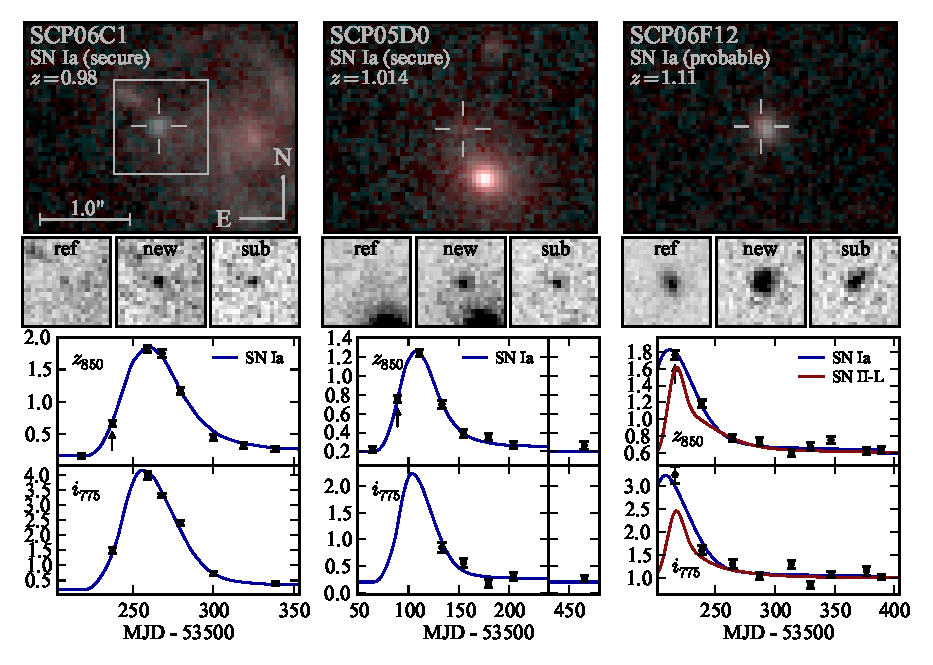
\includegraphics[width=\textwidth]{figures/cands/sn1.eps}
\caption[Images and light curves of candidates classified as
  supernovae.]{Images and light curves of the 29 candidates classified
  as supernovae. For each candidate, the \emph{top panel} shows the
  two-color stacked image ($i_{775}$ and $z_{850}$) of the supernova
  host galaxy, with the SN position indicated. The \emph{three smaller
    panels} below the stacked image show the reference, new, and
  subtracted images for the discovery visit. The \emph{bottom panel}
  shows the light curve at the SN position (including host galaxy
  light) in the $z_{850}$ ({\it top}) and $i_{775}$ ({\it bottom})
  bands. The y axes have units of counts per second in a $3$~pixel
  radius aperture. The effective zeropoints are 23.94 and 25.02 for
  $z_{850}$ and $i_{775}$, respectively. The discovery visit is
  indicated with an arrow in the $z_{850}$ plot. The best-fit SN~Ia
  template is shown in blue. For cases where the type is SN~Ia based
  on spectroscopic confirmation or host galaxy environment, only the
  best-fit SN~Ia template is shown, to demonstrate the consistency of
  the light curve with the designation. For cases where the type is
  based only on the light curve fit, the best-fit core collapse SN
  template is shown in red.  Note that the photometry used here is
  simple aperture photometry with fixed aperture corrections. For
  SN~Ia cosmology we use color-dependent aperture corrections, as
  described in \citet{suzuki11a}. [\emph{continued on next 5 pages.}]
\label{fig:sn}}
\end{figure}

\begin{figure}[p]
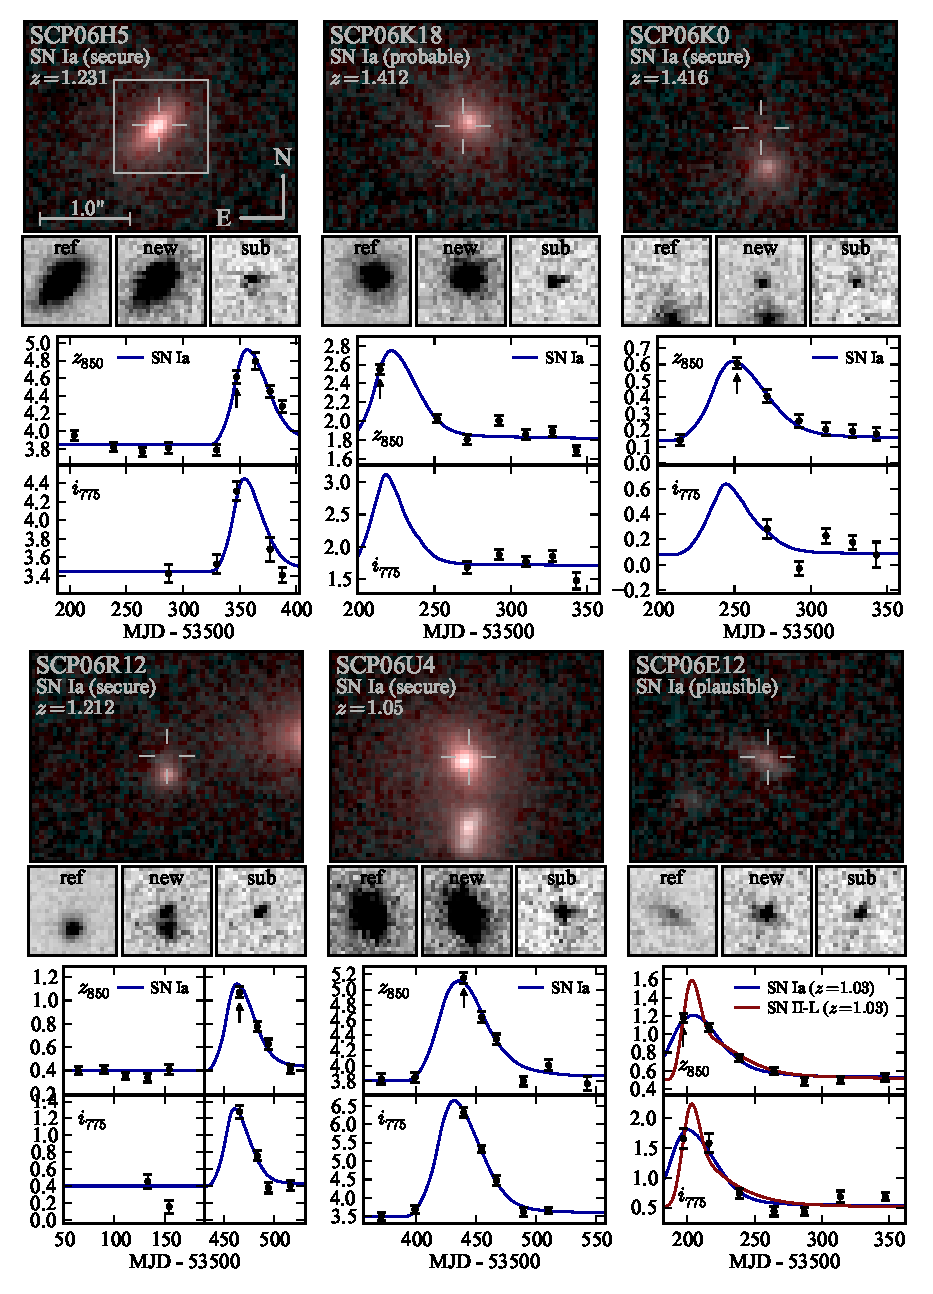
\includegraphics[width=\textwidth]{figures/cands/sn2.eps}
\end{figure}

\begin{figure}[p]
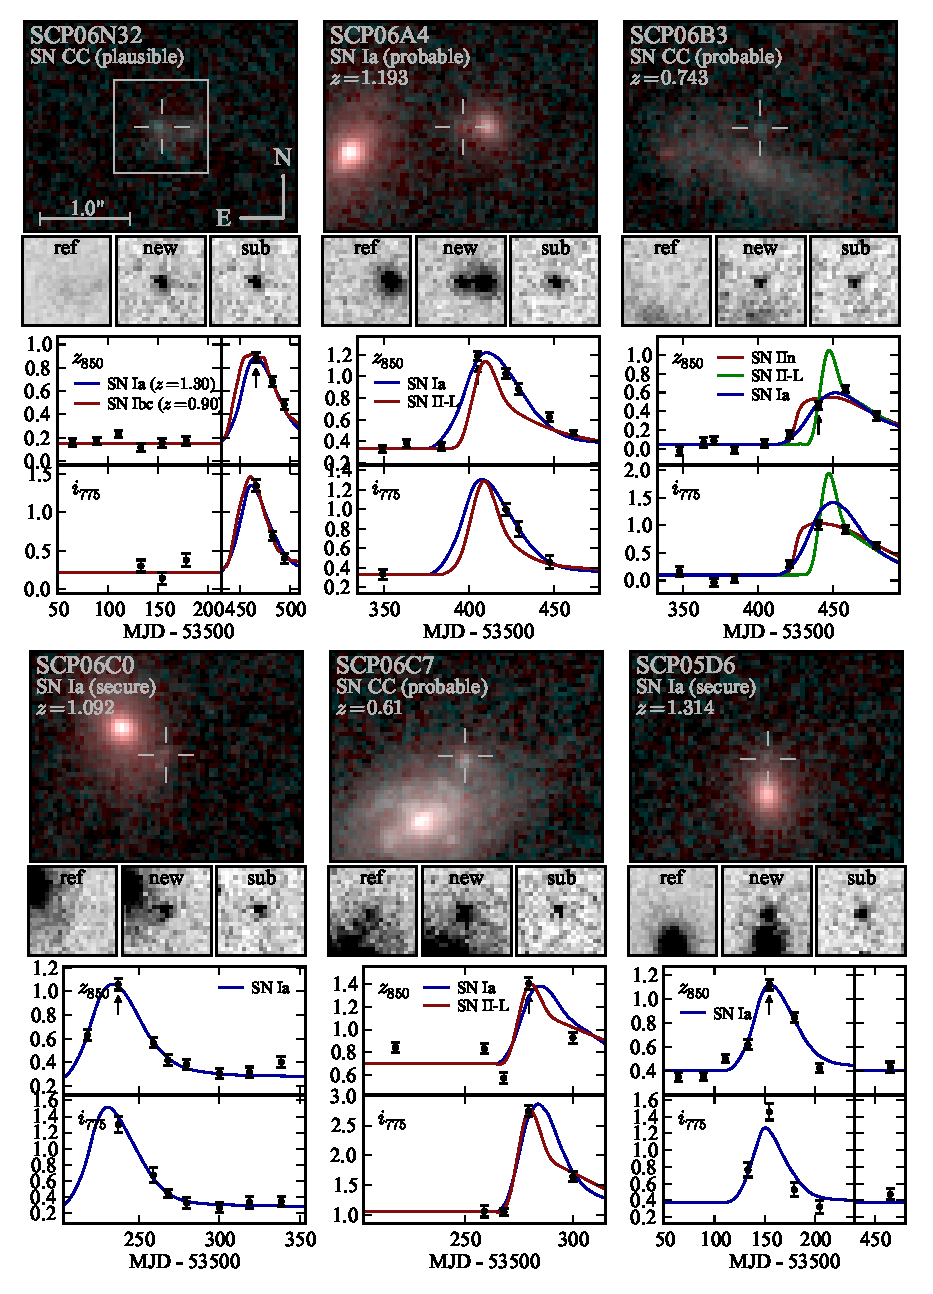
\includegraphics[width=\textwidth]{figures/cands/sn3.eps}
\end{figure}

\begin{figure}[p]
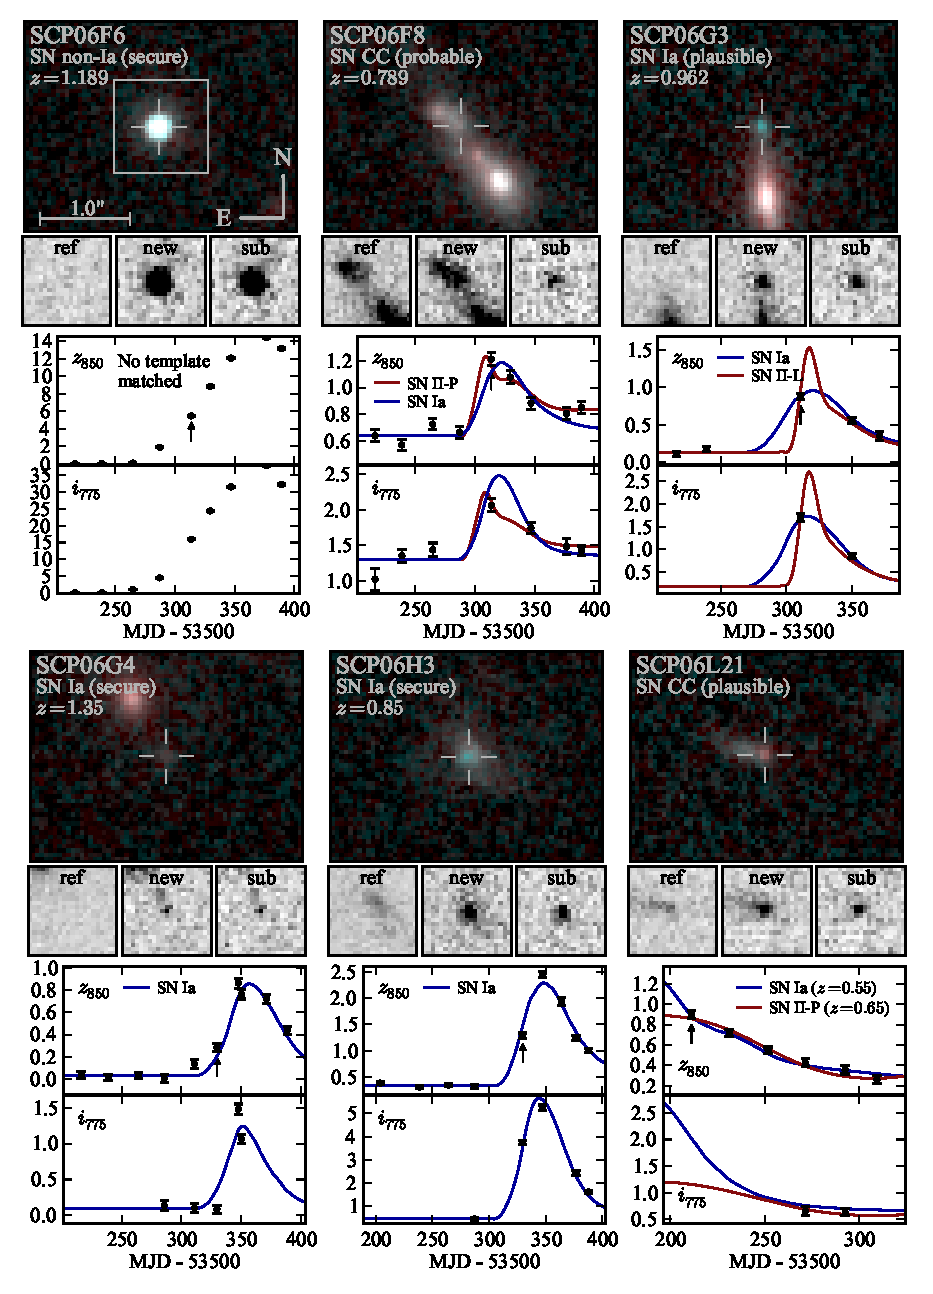
\includegraphics[width=\textwidth]{figures/cands/sn4.eps}
\end{figure}

\begin{figure}[p]
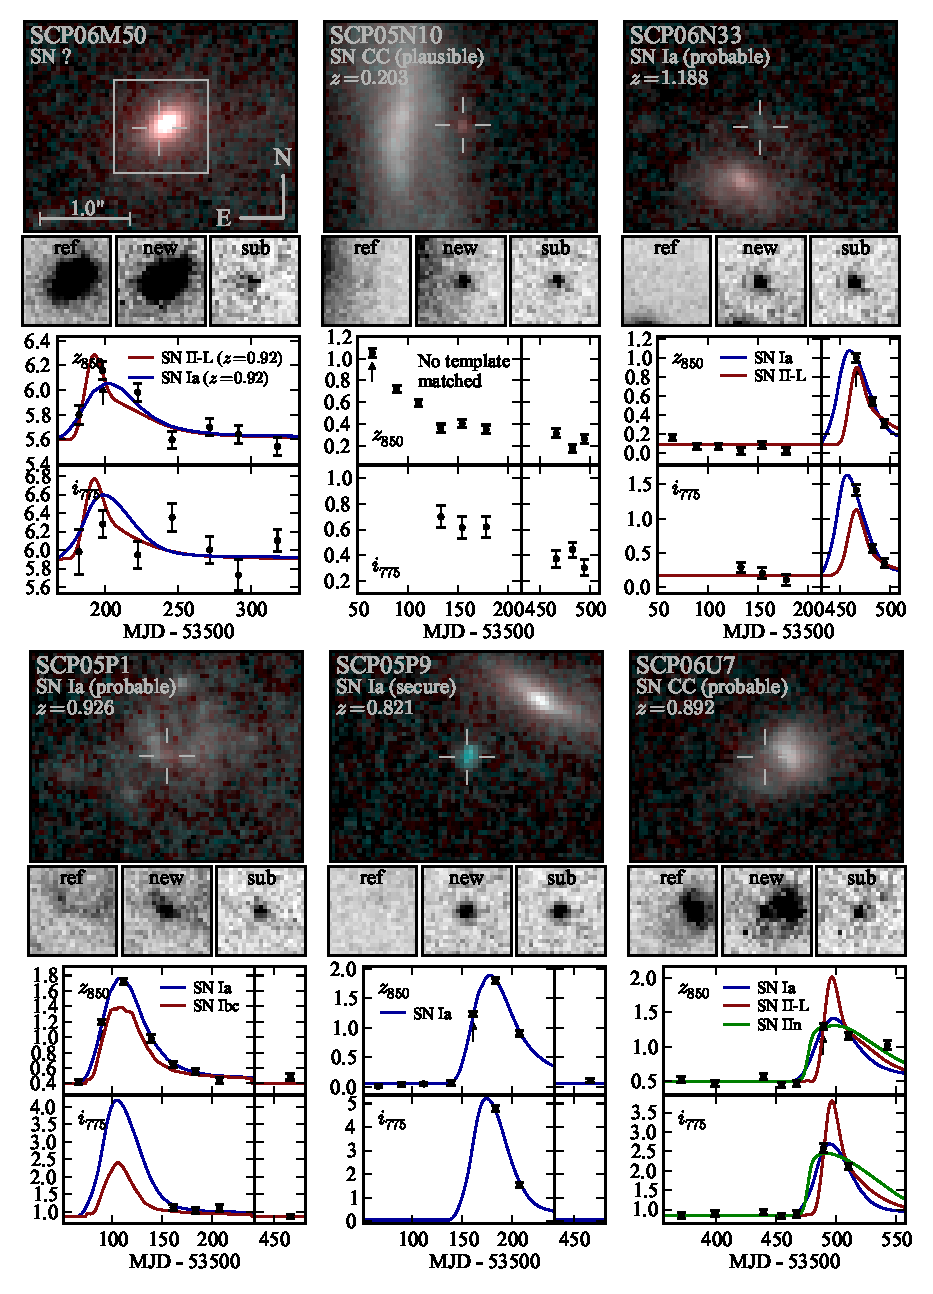
\includegraphics[width=\textwidth]{figures/cands/sn5.eps}
\end{figure}

\begin{figure}[t]
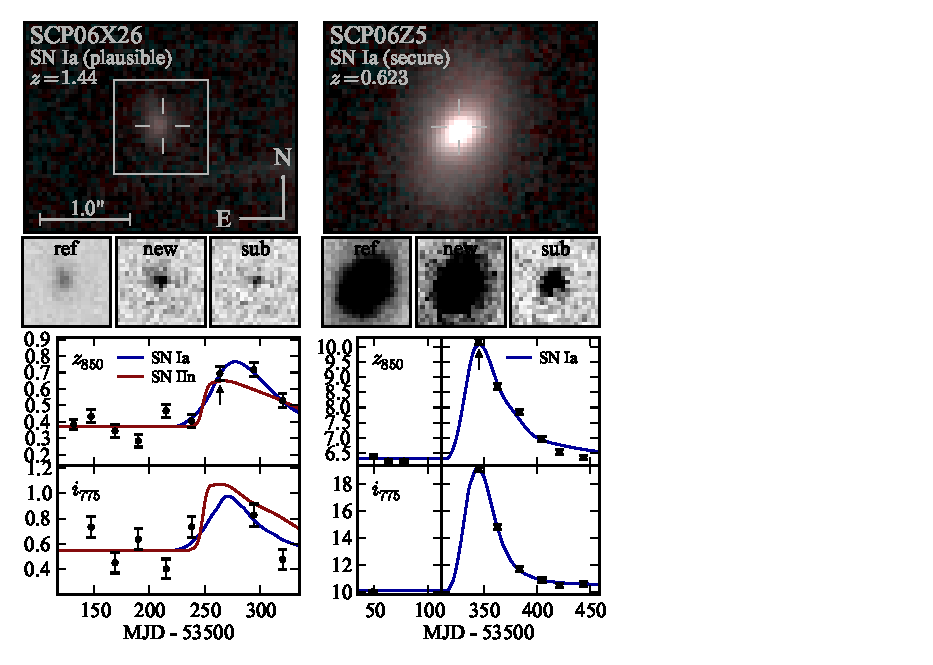
\includegraphics[width=\textwidth]{figures/cands/sn6.eps}
\end{figure}

%%%%%%%%%%%%%%%%%%%%%%%%%%%%%%%%%%%%%%%%%%%%%%%%%%%%%%%%%%%%%%%%%%%%%%%%
% end of SN candidates figures                                         %
%%%%%%%%%%%%%%%%%%%%%%%%%%%%%%%%%%%%%%%%%%%%%%%%%%%%%%%%%%%%%%%%%%%%%%%%


\begin{figure}[t]
\begin{center}
\includegraphics[width=\textwidth]{figures/cands/absmag_vs_z_field.eps}
\end{center}
\caption[Magnitude and redshift distribution of SN
  candidates]{Distribution of SNe in absolute magnitude and redshift,
  based on rough light curve fits. The shading represents the expected
  magnitude distribution of field SNe~Ia (similar for cluster SNe~Ia)
  in the survey in each redshift bin of $\Delta z = 0.05$, based on
  the simulations in \S\ref{sec:fieldrate_ct}. The candidates
  designated as core-collapse are all significantly dimmer than
  expected for SNe~Ia, while the distribution of SN~Ia candidates
  follows the expected distribution closely. Note that the light curve
  of SN SCP06K18 is very poorly constrained: $M_B \gtrsim -19.5$ is
  also consistent with the light curve data.\label{fig:absmag_vs_z}}
\end{figure}


\subsection{Comments on Individual SN Light Curves} 
\label{sec:cands_sncomments}

Here we comment in greater detail on a selection of individual
candidates, particularly those with the greatest uncertainty in
typing. For each candidate, see the corresponding panel of
Figure~\ref{fig:sn} for an illustration of the candidate host galaxy and
light curve.

%{\it SN SCP06F12} is the only cluster-member SN lacking both
%spectroscopic confirmation and an early-type host galaxy, and is thus
%the only cluster-member SN with significant typing uncertainty. The
%light curve is consistent with both SN~Ia and SN Ibc templates (see
%Fig.~\ref{fig:sn}) and to a lesser extent SN II-L. However, the
%best-fit absolute magnitude ($M_B=-19.2$) and color ($c=-0.1$) for the
%SN~Ia template are well within the normal ranges for SNe~Ia, while
%they are fairly extreme for SNe Ibc and II-L. Thus, we classify
%SCP06F12 as a ``plausible'' SN~Ia.

{\it SN SCP06E12}. We were unable to obtain a host galaxy redshift due
to the faintness of the host. The color of the host galaxy is
consistent with the cluster red sequence. The candidate light curve is
consistent with a SN~Ia at the cluster redshift of $z=1.03$, but is
also consistent with SN II-L at $z=1.03$. Different SN types provide
an acceptable fit over a fairly wide range of redshifts. As the SN~Ia
template provides a good fit with typical parameters, we classify the
candidate as a ``plausible'' SN~Ia.  However, there is considerable
uncertainty due to the uncertain redshift.


{\it SN SCP06N32} also lacks a host galaxy redshift. If the cluster
redshift of $z=1.03$ is assumed, the candidate light curve is best fit
by a SN~Ibc template. A SN~Ia template also yields an acceptable
fit, but requires an unusually red color of $E(B-V) \sim 0.6$. Given
the best-fit $s$ and $M_B$ values, the candidate would have an
unusually large Hubble diagram residual of approximately
$-0.8$~magnitudes. If the redshift is allowed to float, a SN~Ia
template with more typical parameters provides an acceptable fit at $z
= 1.3$. A SN~Ibc template still provides a better fit, with the best
fit redshift being $z \sim 0.9$. As SN~Ibc
provides a better fit in both cases, we classify this as a ``plausible''
SN~CC. However, there is considerable uncertainty in
both the type and cluster membership of this candidate. 

{\it SN SCP06A4}. We note that this candidate was observed
spectroscopically, as reported in Dawson09. While the spectrum was
consistent with a SN~Ia, there was not enough evidence to
conclusively assign a type. The host galaxy is morphologically and
photometrically consistent with an early-type galaxy, but there is
detected [O{\sc ii}], a possible indication of star formation. We therefore
rely on light curve typing for this candidate, assigning a confidence
of ``probable'' rather than ``secure.''
 
{\it SN SCP06G3} has only sparse light curve coverage. The best fit
template is a SN~Ia with $s=1.3$, $E(B-V)=0.3$ and $M_B=-18.5$, although
these parameters are poorly constrained. A large stretch and red
color would not be surprising given the spiral nature of the host
galaxy. It is also consistent with a II-L template, although the best
fit color is unusually blue: $E(B-V)=-0.1$. Given that SN~Ia yields
more ``typical'' fit parameters and that, at $z \sim 1$ a detected SN
is more likely to be Type~Ia than II, we classify this as a
``plausible'' Type Ia, with considerable uncertainty in the type.

%{\it SN SCP06F12} is the only cluster-member SN lacking both
%spectroscopic confirmation and an early-type host galaxy, and is thus
%the only cluster-member SN with significant typing uncertainty. The
%light curve is consistent with both SN~Ia and SN Ibc templates (see
%Fig.~\ref{fig:sn}) and to a lesser extent SN II-L. However, the
%best-fit absolute magnitude ($M_B=-19.2$) and color ($c=-0.1$) for the
%SN~Ia template are well within the normal ranges for SNe~Ia, while
%they are fairly extreme for SNe Ibc and II-L. Thus, we classify
%SCP06F12 as a ``plausible'' SN~Ia.

%{\it SN SCP06B3} is too dim ($M_B>-18$) to fit a SN~Ia. Furthermore,
%the $i_{775}$ light curve is much broader than the best-fit SN~Ia. Both
%SN II-P and II-L templates provide a better fit, with regard to shape,
%absolute magnitude and color. \NOTE{GA: Host type?}

%{\it SN SCP06C7} has a light curve too dim, too blue, and too narrow to
%fit a SN~Ia template, even with $s=0.6$, $c=-0.2$ and $M_B=-18.0$
%(shown in Fig.~\ref{fig:sn}). An SN II-L light curve is a far better fit
%with $M_B=-17.2$, $E(B-V)=0.0$. \NOTE{GA: Host type?}

%{\it SN SCP06F8} also has a light curve that clearly favors a SN CC. A
%dim SN~Ia with $M_B=-18.0$ and $s=0.7$ can fit the peak of the
%light curve, but fades too fast in $z_{850}$ to fit the late-time
%light curve. An SN II-P with $M_B=-17.3$, $E(B-V)=0.4$ provides a much
%better fit. For all three of the above SNe, SN SCP06B3, SN SCP06C7 and
%SN SCP06F8, because the light curve clearly favors CC SNe and disfavors
%SNe~Ia, we regard these as ``probable'' SNe CC.

{\it SN SCP06L21} lacks a spectroscopic redshift, but has a distinct
slowly-declining light curve that rules out a $z>0.6$ SN~Ia light
curve. Even the best-fit Ia template at $z=0.55$, shown
in Fig.~\ref{fig:sn}), is unusually dim ($M_B \approx -17.5$), making it
unlikely that the candidate is a lower-redshift SN~Ia. The light curve
is better fit by a SN~II-P template (with the best-fit redshift being
$z=0.65$). We therefore classify the candidate as a ``probable''
SN~CC.

{\it SN SCP06M50} is the most questionable ``SN'' candidate, having no
obvious $i_{775}$ counterpart to the increase seen in $z_{850}$. It
may in fact be an image artifact or AGN. However, it appears to be off
the core of the galaxy by $\sim$2~pixels (making AGN a less likely
explanation), and shows an increase in $z_{850}$ flux in two
consecutive visits, with no obvious cosmic rays or hot pixels (making
an image artifact less likely as well). The galaxy is likely to be a
cluster member: its color and magnitude put it on the cluster red
sequence, it is morphologically early-type, and it is only $19''$ from
the cluster center. Under the assumption that the candidate is a
supernova and at the cluster redshift of $z=0.92$, no template
provides a good fit due to the lack of an $i_{775}$ detection and the
constraints on $E(B-V)$. In particular, a SN~Ia template would
require $E(B-V)>0.6$. (The best-fit template shown in
Fig.~\ref{fig:sn} is with $E(B-V) = 0.6$.) If the redshift is allowed
to float, it is possible to obtain a good fit at higher redshift
($z \sim 1.3$), but still with $E(B-V) \gtrsim 0.4$, regardless of the
template type. Given the color and early-type morphology of the host
galaxy, it is unlikely to contain much dust. There is thus no
consistent picture of this candidate as a SN, and we do not assign a
type. However, note that the candidate is unlikely to be a cluster
SN~Ia.

{\it SN SCP05N10} is the lowest-redshift SN candidate in our sample at
$z=0.203$. Its light curve shape is inconsistent with a SN~Ia occurring
well before the first observation, and its luminosity is too low for
a SN~Ia with maximum only slightly before the first
observation. Therefore, we call this a ``probable'' SN CC. For all SN
types, the best fit requires maximum light to occur well before the
first observation, making all fits poorly constrained.

%{\it SN SCP06N33} is fit quite well by a SN~Ia template with typical
%parameters $c=-0.1$, $s=0.8$, and $M_B=-19.1$. The light curve is too
%blue to be fit by a SN~Ibc template, even with $c=-0.1$. An SN~II-P
%fits near maximum light with $c=-0.1$, but does not decline fast
%enough to fit the last data point. Because a SN~Ia template provides
%a much better fit than other templates, we call this a ``probable''
%SN~Ia.

%{\it SN SCP05P1} has a well-sampled light curve in $z_{850}$, but is
%lacking $i_{775}$ data during the peak of the light curve. An SN~Ia is
%an excellent fit to the data, with $s=1.1$, and $M_B=-19.1$. The only
%SN CC template that also fits the data is a SN Ibc. As the
%parameters are more typical of a SN~Ia (and SNe~Ia are much more
%likely to be discovered at this redshift), we classify this a
%``plausible'' SN~Ia.

%{\it SN SCP06U7} has a slowly-declining light curve, poorly fit by an
%SN~Ia template (see Fig.~\ref{fig:sn}). An SN II-P is the best fit
%template, but requires a color bluer than the template
%($E(B-V)=-0.1$). Because the light curve shape is clearly inconsistent
%with a SN~Ia, we classify this as a ``probable'' SN CC.

{\it SN SCP06X26} has a tentative redshift of $z=1.44$, derived from a
possible [O{\sc ii}] emission line in its host galaxy. Given this redshift,
a Ia template provides an acceptable fit, consistent with a typical
SN~Ia luminosity and color. However, we consider this a ``plausible,''
rather than ``probable,'' SN~Ia, given the uncertain redshift and low
signal-to-noise of the light curve data.

%%%%%%%%%%%%%%%%%%%%%%%%%%%%%%%%%%%%
% TABLE: SN COUNTS AND UNCERTAINTY %
%%%%%%%%%%%%%%%%%%%%%%%%%%%%%%%%%%%%
%\begin{table*}{lccccc}
%\tablewidth{0pt}
%\tablecaption{\label{tab:sncount} SN~Ia counts}
%\tablehead{\colhead{environment} & \colhead{minimum} & \colhead{estimate} & \colhead{maximum} & \colhead{``Secure'' and ``Probable'' SNe~Ia} & \colhead{``Plausible'' SNe~Ia}}
%\startdata
%Cluster Early Type & 6 & 7   & 7  & D0, H5, K0, K18, R12, U4     & E12 \\  
%Cluster            & 7 & 8-9 & 9  & C1, D0, H5, K0, K18, R12, U4 & F12, E12\\
%Field $0.2<z<0.6$  & 0 & 0   & 0  & \nodata                      & \nodata \\
%Field $0.6<z<1.0$  & 3 & 5   & 6  & Z5, P9, H3                   & P1, G3, E12 \\
%Field $1.0<z<1.4$  & 5 & 5   & 7  & A4, C0, D6, G4, N33          & E12, N32 \\
%Field $z>1.4$      & 0 & 1   & 1  & \nodata                      & X26
%\enddata
%\end{table*}




%%%%%%%%%%%%%%%%%%%%%%%%%%%%%%%%%%%%%%%%%%%%
% Chapter 5: Cluster Rate Calculation      %
%%%%%%%%%%%%%%%%%%%%%%%%%%%%%%%%%%%%%%%%%%%%
\chapter{Cluster Rate} \label{sec:clrate}

\section{Overview of Calculation} \label{sec:clrate_overview}

With the systematically selected SN sample from the previous chapter,
we are now in a position to calculate SN rates. The cluster SN~Ia rate
is given by
\begin{equation}
\label{eq:rate}
\mathcal{R} = \frac{N_{\rm SN~Ia}}{\sum_j T_j L_j} ,
\end{equation}
where $N_{\rm SN~Ia}$ is the total number of SNe~Ia observed in
clusters in the survey, and the denominator is the total effective
time-luminosity for which the survey is sensitive to SNe~Ia in
clusters. $L_j$ is the luminosity of cluster $j$ visible to the survey
in a given band. $T_j$ is the ``effective visibility time'' (also
known as the ``control time'') for cluster $j$. This is the effective
time for which the survey is sensitive to detecting a SN~Ia,
calculated by integrating the probability of detecting a SN~Ia as a
function of time over the span of the survey. It depends on the
redshift of the SN~Ia to be detected and the dates and depths of the
survey observations. As each cluster has a different redshift and
different observations, the control time is determined separately for
each cluster.  To calculate a rate per stellar mass, $L_j$ is replaced
by $M_j$.

Equation~(\ref{eq:rate}) is for the case where the entire observed
area for each cluster is observed uniformly, yielding a control time
$T$ that applies to the entire area.  In practice, different areas of
each cluster may have different observation dates and/or depths,
resulting in a control time that varies with position. This is
particularly true for this survey, due to the rotation of the observed
field between visits and the gap between ACS chips. Therefore, we
calculate the control time as a function of position in each observed
field, $T_j(x,y)$. As the cluster luminosity is also a function of
position, we weight the control time at each position by the
luminosity at that position. In other words, we make the substitution
\begin{equation} 
\label{eq:ratedenom}
T_j L_j \Rightarrow \int_{x,y} T_j (x,y) L_j (x,y). 
\end{equation}

In \S\ref{sec:clrate_candsummary} we summarize the findings of the
previous chapter for $N_{\rm SN~Ia}$.  In \S\ref{sec:ct} we calculate
$T_j (x,y)$, and in \S\ref{sec:lum} we calculate $L_j(x,y)$.



\section{Summary of Cluster SN Candidates} \label{sec:clrate_candsummary}
In the previous chapter we addressed the type of all 29 candidates
thought to be SNe. However only the cluster-member SNe~Ia are of
interest for this chapter. There are six ``secure''
cluster-member SNe~Ia, and two ``probable'' SNe~Ia, for a total of
eight. In addition, SCP06E12 is a ``plausible'' SN~Ia and may be a
cluster member. Two other candidates, SCP06N32 and SCP06M50, cannot be
definitively ruled out as cluster-member SNe~Ia, but are quite
unlikely for reasons outlined above. We take eight cluster SNe~Ia as
the most likely total. It is unlikely that {\it both} of the
``probable'' SNe~Ia are in fact SNe~CC. We therefore assign a
classification error of $^{+0.0}_{-0.5}$ for each of these, resulting
in a lower limit of seven cluster-member SNe~Ia. There is a good
chance that SCP06E12 is a cluster-member SN~Ia, while there is only a
small chance that SCP06N32 and SCP06M50 are either cluster SNe~Ia. For
these three candidates together, we assign a classification error of
$^{+1}_{-0}$, for an upper limit of nine. Thus, $8 \pm 1$ is the total
number of observed cluster SNe~Ia, including classification uncertainty.



%%%%%%%%%%%%%%%%%%%%% Control Time %%%%%%%%%%%%%%%%%%%%%%%%%%%%
\section{Effective Visibility Time} \label{sec:ct}

The effective visibility time $T$ at a position $(x,y)$ on the 
sky is given by
\begin{equation}
T(x,y) = \int_{t=-\infty}^{t=\infty} \eta^\ast (x,y,t) \epsilon (x,y,t) dt.
\end{equation}
The integrand here is simply the probability for the survey and our
selection method to detect (and keep) a SN~Ia at the cluster redshift
that explodes at time $t$, and position $(x,y)$. This probability is
split into the probability $\eta^\ast$ of detecting the supernova and
the probability $\epsilon$ that the supernova passes all ``light
curve'' cuts. As each SN has multiple chances for detection, the total
probability of detection $\eta^\ast$ is a combination of the
probabilities of detection in each observation. For example, if we
have two search visits at position $(x,y)$, $\eta^\ast(t)$ is given by
\begin{equation}
\eta^\ast (t) = \eta_1 (t)+ ( 1-\eta_1(t) ) \eta_2 (t),
\end{equation}
where $\eta_i (t)$ is the probability of detecting a SN~Ia 
exploding at time $t$ in visit $i$. In other words, the total 
probability of finding the SN~Ia exploding at time $t$ is the probability 
of finding it in visit 1 plus the probability that it was \emph{not} found in
visit 1 times the probability of finding it in visit 2. This can be 
generalized to many search visits: The contribution of each additional visit 
to the total probability is the probability of not finding the SN in any 
previous visit times the probability of finding the SN in that visit.

In practice, we calculate $T(x,y)$ in two steps: First, we determine
the probability $\eta$ of detecting a new point source in a single
image as a function of the point source magnitude. This is discussed
in \S\ref{sec:ct_eff}. Second, for each $(x,y)$ position in the observed area
we simulate a variety of SN~Ia light curves at the cluster redshift
occurring at various times during the survey. By considering the dates
of the observations made during the survey at that specific position,
we calculate the brightness and significance each simulated SN~Ia would
have in each $z_{850}$ and $i_{775}$ image. We then use our
calculation of $\eta$ as a function of magnitude to convert the
observed brightness into a probability of detecting the simulated SN
in each observation. The light curve simulation is discussed in
\S\ref{sec:ct_mc}. 


\subsection{Detection Efficiency} \label{sec:ct_eff}
%%%%%%%%%%%%%%%%%%%%%%%%%%%%
% OLD TEXT : Use in thesis %
%%%%%%%%%%%%%%%%%%%%%%%%%%%%

Here we calculate the probability of detecting a new point source as a
function of magnitude.  We use a Monte Carlo simulation in which
artificial point sources of various magnitudes are added to survey
images. The images are then run through the same reduction and SN
detection pipeline used in the search.

Because our search procedure uses information from individual
exposures to reject cosmic rays, it is necessary to place the
artificial point sources on these individual exposure images rather
than on the combined image from each visit. This allows us to test
both the efficiency of the {\sc MultiDrizzle} process and our CR
rejection. We add the artificial point sources to the raw CCD images
after bias subtraction and flat fielding. As these ``\texttt{\_flt}''
images have not been re-sampled, they accurately represent the light
on each CCD pixel.

As a model of the point spread function (PSF) on these images, we use
the PSF library of \citet{anderson06a}. For each of six ACS filters,
this library represents the position-dependent PSF by a $9 \times 10$
array of fiducial PSFs across the two CCDs. Each fiducial PSF model is
oversampled by a linear factor of 4, giving the model a pixel scale of
$0''.0125$. As this library was derived on \texttt{\_flt} images, it
is directly applicable to these images.

The artificial point sources are placed on galaxies according to the
distribution of light in each galaxy. Galaxies with $z_{850} < 20$ are
not used, as these are only found at redshifts below the range of
interest. Only one point source is placed on each galaxy to avoid
detection complications from overlapping sources.  Once a position on
a galaxy is chosen, it is converted to a corresponding CCD chip
position on each of the (typically four) individual exposure images
taken for the visit.  The oversampled fiducial PSF model for this
position on the CCD is chosen from the PSF library and is re-sampled
onto the CCD pixels. A random point source flux is drawn from the
range of interest. The PSF model is adjusted to match this flux. It is
normalized so that the encircled energy in a 3~pixel radius aperture
in the combined image matches the value derived
by \citet{sirianni05a}.  A further adjustment to the flux is made to
compensate for the variation in effective pixel area across the
detector. (This variation is due to the ACS distortion and is on the
order of 10 to 20\%.) Poisson noise is added to each pixel in the PSF
and the PSF is then added to the image.  Images are passed through the
same reduction and detection pipeline used in the search. Finally, the
flagged candidates are compared to the input artificial point sources.

%%%%%%%%%%%%%%%%%%%%
% PLOT: EFFICIENCY %
%%%%%%%%%%%%%%%%%%%%
\begin{figure}[t]
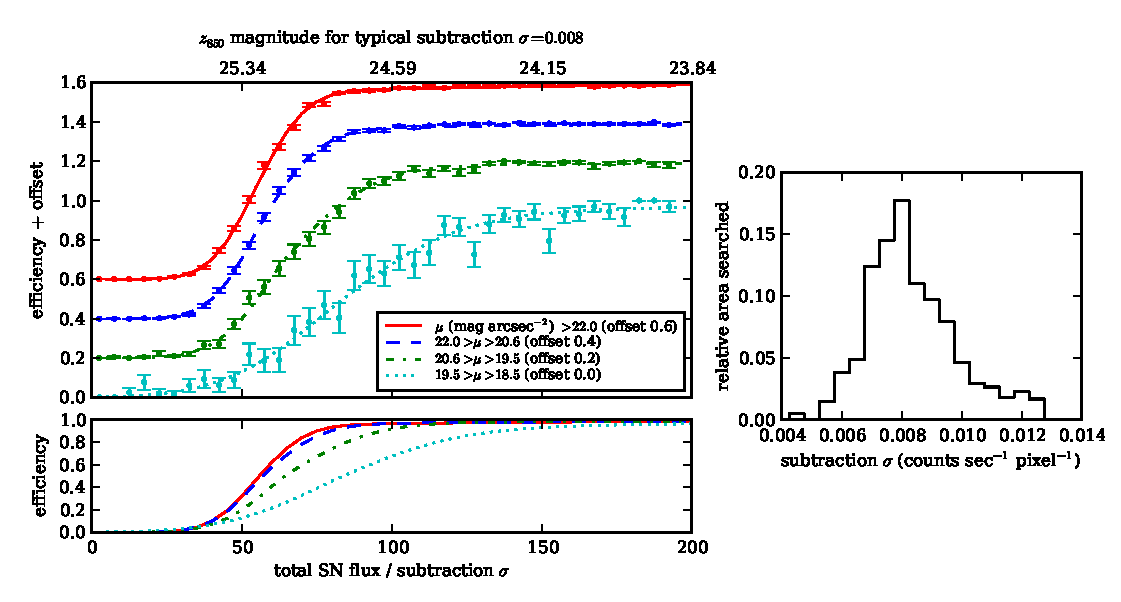
\includegraphics[width=\textwidth]{figures/clrate/eff_color.eps}
\caption[Point source detection efficiency]{Point source detection 
efficiency in a single subtraction, 
as a function of the ratio of total point source flux to subtraction
noise $\sigma$ (counts~sec$^{-1}$~pixel$^{-1}$). The artificial point
sources are split into four bins depending on the underlying galaxy
surface brightness $\mu$ (mag~arcsec$^{-2}$) at the point source
position. The efficiency curve is calculated separately for each
bin. In the \emph{upper left panel}, the four bins are shown, offset for
clarity. In the \emph{lower left panel}, the fitted curves are reproduced
without offset for comparison. Approximately 72,000 artificial point
sources were used in total. The \emph{right panel} shows the distribution of
the noise level in the subtractions. The noise level differs by a
factor of about two from the deepest to shallowest subtractions
searched.\label{fig:eff}}
\end{figure}

%The detection efficiency
%The noise level varies between subtractions and between different
%regions within a single subtraction.  To avoid running a full Monte
%Carlo simulation for each of these subtractions and regions, 

We parameterize the detection efficiency by the ratio of point source
flux to sky noise. This is a good choice because, in most cases, the
detection efficiency will depend only on the contrast between the
point source and the sky noise. However, there is an additional
dependence on the surface brightness at the location of the point
source: point sources near the core of galaxies will have a lower
detection efficiency due to additional Poisson noise from the
galaxy. For $0.6<z<1.5$ galaxies, we estimate that only $\sim$$10\%$
of SNe will fall on regions where galaxy Poisson noise is greater than
the sky noise (assuming SNe follow the galaxy light
distribution). Still, we take this effect into account by splitting
our sample of artificial point sources into four bins in underlying
surface brightness. The detection efficiency is calculated separately
in each bin (Fig.~\ref{fig:eff}, top left panel).  The first two bins,
$\mu > 22.0$ and $22.0 > \mu > 20.6$ mag~arcsec$^{-2}$, correspond to
lower surface brightnesses where sky noise is dominant. As expected,
their efficiency curves are very similar. In the third and fourth
bins, corresponding to higher surface brightness, the Poisson noise
from the galaxy dominates the sky noise, and the efficiency drops as a
result.

For reference, the distribution of sky noise in the subtractions is
shown in Figure~\ref{fig:eff} (right panel). Nearly all the searched
area has a sky noise level between 0.006 and
0.012 counts sec$^{-1}$ pixel$^{-1}$. For a typical value of 0.008, we
show the corresponding point source $z_{850}$ magnitude on the top
axis of the left panel.

We find that the efficiency curve in each bin is well-described by
the function
\begin{equation}
\eta(x) = \left\{ \begin{array}{ll}
\frac{1}{2} (1+ae^{-bx}) [\mathrm{erf}((x-c)/d_1)+1], & x<c     \\
\frac{1}{2} (1+ae^{-bx}) [\mathrm{erf}((x-c)/d_2)+1], & x \ge c
\end{array} \right. ,
\end{equation}
where $x$ is the ratio of point source flux to sky noise, and $a$,
$b$, $c$, $d_1$ and $d_2$ are free parameters. An error function is
the curve one would expect with a constant cut and Gaussian noise, but
we find that two different scales ($d_1$ and $d_2$) in the error
function, as well as an additional exponential term, are necessary to
describe the slow rise to $\eta =1$ at large $x$. This slow rise is
due to rarer occurrences, such as cosmic rays coinciding with new point
sources. The fitted functions for the four bins are plotted in the top
left of Figure~\ref{fig:eff} and reproduced in the bottom left of the
figure for comparison. We use these fitted functions to calculate the
effective visibility time in the following section. 


\subsection{Simulated Lightcurves} \label{sec:ct_mc}

%For each cluster, the control time at each position in the observed
%area, $T(x,y)$, is calculated with a Monte Carlo simulation. We
%simulate SN~Ia light curves at the cluster redshift at various times
%during the survey, and determine the probability (using the detection
%efficiencies from Fig.~\ref{fig:eff}) that each simulated SN would be
%detected and counted in our SN sample.

We simulate SN~Ia light curves with a distribution of shapes, colors
and absolute magnitudes.  We use the (original) {\sc
salt} \citep{guy05a} prescription in which the diversity of SN~Ia
light curves is characterized as a two-parameter family with an
additional intrinsic dispersion in luminosity.  The two parameters are
the linear timescale of the light curve (``stretch'', $s$) and the
$B-V$ color excess, $c$.  For each simulated SN, $s$ and $c$ are
randomly drawn from the distributions shown in Figure~\ref{fig:dists}
(solid lines). The stretch distribution is based on the
observed distribution in passive hosts
(Fig.~\ref{fig:dists}, left panel, grey histogram) in the
first-year Supernova Legacy Survey (SNLS) sample \citep{sullivan06a}.
Similarly, the color distribution is based on the observed color
distribution (Fig.~\ref{fig:dists}, right panel, grey
histogram) in the first-year SNLS sample \citep{astier06a}.  The
absolute magnitude of each simulated SN is set to
\begin{equation}
M_B = -19.31 - \alpha (s-1) + \beta c + I
\end{equation}
where $-19.31$ is the magnitude of an $s=1$, $c=0$ SN~Ia in our
assumed cosmology \citep{astier06a}, $\alpha = 1.24$, $\beta =
2.28$ \citep{kowalski08a}, and $I$ is an added ``intrinsic
dispersion'', randomly drawn from a Gaussian distribution centered at
zero with $\sigma = 0.15$~mag.

%%%%%%%%%%%%%%%%%%%%%%%%%%%%%%%%%%
% PLOT: SIMULATION DISTRIBUTIONS %
%%%%%%%%%%%%%%%%%%%%%%%%%%%%%%%%%%
\begin{figure}[tbhp]

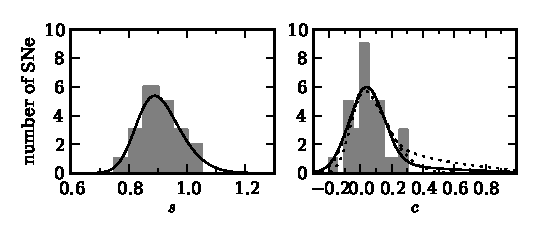
\includegraphics[width=\textwidth]{figures/clrate/dists_cluster.eps}
\caption[Stretch and color distributions of simulated supernovae]
{{\it Left panel:} stretch distribution used for simulated SNe 
(solid line) and the stretch distribution of first-year SNLS
$z<0.75$ SNe in passive hosts \citep{sullivan06a} (grey
histogram). Note that the distribution is not changed significantly
by cutting the sample at $z<0.6$. Therefore we do not expect the
sample to be significantly Malmquist biased. {\it Right panel:} color
distribution of the first-year SNLS $z<0.6$ SNe \citep{astier06a}
(grey histogram) and the color distribution used for simulated
SNe (solid line). The dotted lines show alternative
color distributions used to assess the possible systematic error due
to varying amounts of SNe being affected by dust.\label{fig:dists}}
\end{figure}

We have chosen distributions that represent as accurately as possible
the full distribution of SNe~Ia occurring in reality. However, note
that the control time is not actually very sensitive to the assumed
distributions. This is because, for the majority of cluster redshifts
in the survey, the detection efficiency is close to 100\% during the
time of the survey. Supernovae would thus have to be significantly
less luminous in order to change the detection efficiency
significantly. In the following section \S\ref{sec:ct_sys} we quantify the
effect on the control time arising from varying the assumed SN~Ia
properties and show that they are sub-dominant compared to the Poisson
error in the number of SNe observed. All sources of systematic errors
are also summarized in \S\ref{sec:clrate_results_sys}.

To generate the simulated light curves in the observed bands, we use
the \citet{hsiao07a} SN~Ia spectral time series template. For each
simulated SN, the spectral time series is warped to match the selected
color $c$ and redshifted to the cluster rest-frame. Light curves are
generated in the observed $i_{775}$ and $z_{850}$ filters using
synthetic photometry, and the time axis is scaled according to the
chosen value of $s$.

For each cluster, we calculate $T(x,y)$ in bins of 50 $\times$
50~pixels ($2''.5\ \times\ 2''.5$). In each bin, we simulate 100 SN
light curves at random positions within the bin.  For each simulated
SN light curve, we shift the light curve in time across the entire
range of observations, starting with maximum light occurring 50~days
before the first observation and ending with maximum light occurring
50~days after the last observation. For each step in time we get the
$z_{850}$ and $i_{775}$ magnitude of the SN at every date of
observation. From the sky noise maps, we know the noise at the
position of the simulated SN in every image. Using the curves in
Figure~\ref{fig:eff}, we convert the SN flux-to-noise ratio to the
probability of the SN being detected in each $z_{850}$ exposure. (Each
simulated SN is also assigned a host galaxy surface brightness chosen
from a distribution, in addition to the randomly selected $s$, $c$ and
$I$ parameters; we use the Fig.~\ref{fig:eff} curve that corresponds
to this surface brightness.) At the same time, we calculate the
probability that the SN passes our light curve cuts (using both
$z_{850}$ and $i_{775}$ simulated magnitudes). Multiplying these two
probabilities gives the total probability of the simulated SN being
included in the sample if it peaks at the given date.  Integrating the
probability over time (the entire range of dates) gives the control
time for each simulated SN. We take the average control time of the
100 SNe as the value for the given bin. The resulting control time
map, $T(x,y)$, therefore has a resolution of $2''.5\ \times\
2''.5$. $T(x,y)$ is shown for two example clusters in
Figure~\ref{fig:ctmaps}.

%%%%%%%%%%%%%%%%%%%%%%%%%%%%%%%%%%
% PLOT: CTMAPS                   %
%%%%%%%%%%%%%%%%%%%%%%%%%%%%%%%%%%
\begin{figure}

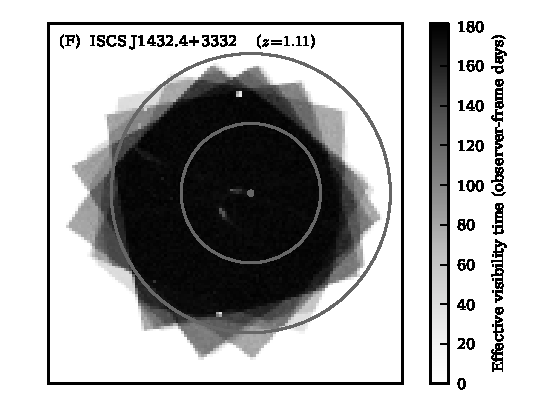
\includegraphics[width=0.5\textwidth]{figures/clrate/ctmap_f.eps}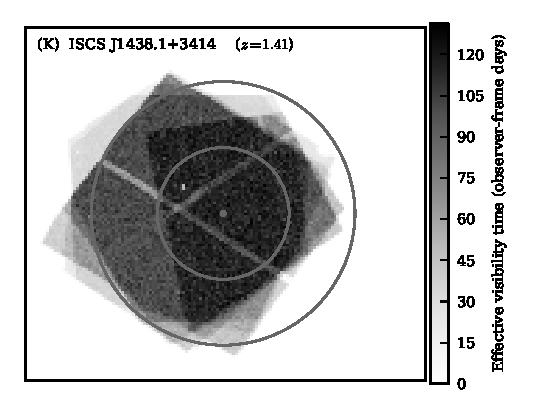
\includegraphics[width=0.5\textwidth]{figures/clrate/ctmap_k.eps}
\caption[Example maps of effective visibility times]
{Example maps of effective visibility time for clusters 
ISCS J1432.4+3332 (F) and ISCS J1438.1+3414 (K).  The dot denotes the
cluster center and the inner and outer circles represent 0.5~Mpc and
1.0~Mpc radius, respectively. The ``noise'' in these maps is due to
the finite number (100) of SNe simulated at each position.  At lower
redshift nearly all simulated SNe are recovered at each position,
whereas at higher redshift a sizable fraction of simulated SNe are
missed, resulting in a higher ``noise'' level.
\label{fig:ctmaps}}
\end{figure}


\subsection{Effect of Varying SN Properties} \label{sec:ct_sys}

If the real distributions of SN~Ia properties differs significantly
from those assumed in our simulation, the $T(x,y)$ maps we have
derived could misrepresent the true efficiency of the survey. Above we
argued that the effect is likely to be small because the detection
efficiency is close to 100\% for most of the survey. Here we quantify
the size of the possible effect on the control time by varying the
assumed distributions.

To first order, changing the assumed distributions of $s$ or $c$ or
changing the assumed spectral time series will affect the detection
efficiency by increasing or decreasing the luminosity of the simulated
SN. To jointly capture these effects, we shift the absolute magnitude
of the simulated SNe~Ia by $^{+0.2}_{-0.2}$~mag and recalculate the
control times. To first order, this is equivalent to shifting the $s$
distribution by $\Delta s = 0.2/\alpha \sim 0.16$ or shifting the $c$
distribution by $\Delta c = 0.2/\beta \sim 0.09$. A $-0.2$~mag shift
in absolute magnitude increases the control time, decreasing the
inferred SN~Ia rate by $6\%$. A $+0.2$~mag shift decreases the control
time, increasing the SN~Ia rate by $8\%$. These effects are
sub-dominant compared to the Poisson error of $\gtrsim 30\%$ in the
number of SNe observed. (Sources of error are summarized
in \S\ref{sec:clrate_results_sys} and Table~\ref{tab:clrate_sys}.)

% EXPLANATION OF SPECTRAL TIME SERIES CHOICE
%To generate the simulated light curves in the observed bands, we use
%the \citet{hsiao07a} SN~Ia spectral time series template.
%This template is known to have higher fidelity in the rest-frame UV
%than, e.g., the {\sc salt}
%\citep{guy05a} or \citet{nugent02a} templates. An accurate UV SN
%template is particularly important here, as the observed $z_{850}$
%band corresponds to rest-frame $U$-band at $z \sim 1.4$.  

%EXPLANATION OF STRETCH DISTRIBUTION
%We keep in mind that clusters are dominated
%by passive galaxies, which preferentially host lower-stretch SNe: we
%base our stretch distribution on the first-year Supernova Legacy
%Survey (SNLS) sample of $z<0.75$ SNe in passive hosts \citet{sullivan06a}.

%EXPLANATION OF COLOR DISTRIBUTION
%For color, we follow a similar approach, but base
%our distribution on the full first-year SNLS sample \citep{astier06a}
%of $z<0.6$ SNe in all host types (the observed $c$ distribution is not
%significantly different in early-type hosts). \citep[e.g.,][]{sullivan10a}
%We have cut the sample at $z<0.6$ to minimize Malmquist bias against
%redder SNe.  The $c$ distribution of these SNe is reproduced in the
%left panel of Figure~\ref{fig:dists} (solid line).

For the color distribution, in addition to a simple shift, we also
quantify the effect of including a smaller or larger fraction of SNe
significantly reddened by dust. In fact, we have good reasons to
believe that most cluster SNe~Ia will be in dust-free environments. A
large fraction of the stellar mass in the clusters ($\sim 80\%$) is
contained in red-sequence galaxies expected to have little or no
dust. Our spectroscopic and photometric analysis \citep{meyers11a} of
the red-sequence galaxies confirms this expectation. Therefore, for
our default $c$ distribution (Fig.~\ref{fig:dists}, right panel, solid
line), we assumed that $20\%$ of SNe (those occurring in galaxies not
on the red sequence) could be affected by dust, and that the
extinction of these SNe would be distributed according to
$P(A_V) \propto \exp(-A_V/0.33)$. This distribution is based on the
inferred underlying $A_V$ distribution of the SDSS-II
sample \citep[][hereafter K09]{kessler09a}. All SNe are assumed to
have an intrinsic dispersion in color to match the observed SNLS
distribution at $c<0.3$. It might be the case that even fewer SNe are
affected by dust, or (unlikely) more SNe are affected by dust. As
extreme examples, we tested two alternative distributions (dotted
lines in Fig.~\ref{fig:dists}). In the first, we assumed that the SNLS
sample was complete and characterized the full $c$ distribution, with
a negligible number of $c>0.4$ SNe. This increases the control time by
only $2\%$. In the second, we increase the fraction of dust-affected
SNe from $20\%$ to $50\%$.  Even though this alternative distribution
includes an additional $\sim$$30\%$ more reddened SNe (unlikely to be
true in reality), the average control time is only lower by $9\%$
(increasing the rate by $10\%$). We use these values as the systematic
error in the assumed dust distribution.


%The assumed distribution of SN color used in the Monte Carlo
%simulation was based on the SNLS $z<0.6$ sample, which contained no
%SNe redder than $c=0.3$. As a result, our assumed $c$ distribution has
%only a very small number of SNe with $c>0.4$. There are two reasons
%that we expect this to be a good representation of reality. First, the
%SNLS sample is reasonably complete at $z<0.6$; if there were many
%$c>0.4$ SNe in reality, some would be found at lower
%redshifts. Note that the trend of no detected $c>0.4$ SNe continues
%in the third-year SNLS sample \citep{sullivan10a}. Second, the stellar
%mass in clusters is predominantly found in early-type galaxies which
%are expected to have less dust than field galaxies. Of course, this
%doesn't mean there are {\it no} high-extinction SNe~Ia in the clusters;
%high-extinction SNe~Ia have been detected in other surveys, and clusters
%do contain some dusty galaxies. However it does mean that there are
%likely a negligible number of $c>0.4$ SNe~Ia occurring in the clusters.

%Still, to test the effect of the existence of high-extinction SNe on
%our control time, we replace our assumed $c$ distribution with one
%including a number of redder SNe. We conservatively assumed that
%$50\%$ of cluster SNe could be affected by dust, and that the
%extinction of these SNe would be distributed according to
%$P(A_V) \propto \exp(-A_V/0.33)$. This is the inferred underlying
%$A_V$ distribution of the SDSS-II sample \citep{kessler09a}. We
%convert this to a distribution in $c$ ($c = A_V/(\beta-1)$) and add
%intrinsic SN color scatter to reach the distribution shown in
%Fig.~\ref{fig:dists} (dotted line). This distribution roughly matches
%our nominal one in the range $-0.2 < c < 0.3$, but includes an
%additional $\sim$$40\%$ more reddened SNe. Using this alternate
%distribution in our simulation, the average control time is lower by
%$10.5\%$. (The effect is greater for higher-redshift clusters and
%smaller for lower-redshift clusters, where SNe are more easily
%detected.) Across all clusters, we would detect the majority of the
%additional $40\%$ more-reddened SNe. Conservatively, we include a
%one-sided control time systematic error of $10.5\%$ in our result.



%%%%%%%%%%%%%%%%%%%% Luminosities %%%%%%%%%%%%%%%%%%%%%%%%%%%%%
\section{Cluster Luminosities and Masses} \label{sec:lum}

In this section, we calculate the total luminosity of each cluster and
use the luminosity to infer a stellar mass. Only a small subset of
galaxies in each field have known redshifts, making it impossible to
cleanly separate cluster galaxies from field galaxies.  Therefore, we
use a ``background subtraction'' method to estimate cluster
luminosities statistically: we sum the luminosity of all detected
galaxies in the field and subtract the average ``background
luminosity'' in a non-cluster field.  This approach follows that
of \citet{sharon07a}.  For the blank field, we use the
GOODS\footnote{Based on observations made with the NASA/ESA 
\emph{Hubble Space Telescope}. The observations are associated with programs
GO-9425, GO-9583 and GO-10189} \citep{giavalisco04a} fields as they
have similarly deep or deeper observations in both ACS $i_{775}$ and
$z_{850}$.

In \S\ref{sec:lum_background} we describe the estimation of image
backgrounds, which must be subtracted to avoid biasing photometry
measurements. \S\ref{sec:lum_photometry} describes the galaxy
detection and photometry method.  Simply summing the photometry from
the detected galaxies would include most of the total cluster
light. However, for an unbiased estimate of the total light, several
small corrections are necessary: We account for light in the outskirts
of each galaxy (\S\ref{sec:lum_correction}), and light from faint
galaxies below the detection threshold
(\S\ref{sec:lum_faintgals}). These corrections are on the order of
20\% and 5\% respectively. In \S\ref{sec:lum_kcorr} we convert the
observed $z_{850}$ flux to a rest-frame $B$-band
flux. \S\ref{sec:lum_centers} describes the method for determining the
center of a cluster. In \S\ref{sec:lum_profiles} we sum the light and
subtract light from non-cluster galaxies, creating a profile of
cluster light as a function of radius. In \S\ref{sec:lum_subsets} we
repeat this calculation limiting ourselves to red-sequence and
red-sequence early-type subsets of galaxies. Finally,
in \S\ref{sec:lum_mass} we estimate cluster stellar masses based on
the cluster luminosities and stellar mass-to-light ratios.


\subsection{Image Background Subtraction} \label{sec:lum_background}

Any residual image background will bias derived galaxy magnitudes. We
use a custom background subtraction algorithm to take out any residual
large-scale varying background. We start with stacked images produced
by {\sc MutiDrizzle}. The individual images are already background
subtracted prior to the {\sc MultiDrizzle} process, but we find that
the stacked images have a small positive mean background.

Objects are detected with Source Extractor 
\citep[{\sc SExtractor};][]{bertin96a} using the standard
one-pass, single-image mode. {\sc SExtractor} is allowed to determine
its own spatially-varying image background, solely for the purposes of
object detection and object geometry. The relevant detection
parameters are given in Table~\ref{tab:sextractor}. A mask is then
created based on the {\sc SExtractor} catalog -- all pixels inside an
object's MAG\_AUTO aperture are masked. In particular, note that
PHOT\_AUTOPARAMS is set to [8.0, 3.3]. This means that each object is
masked out to 8 times its Kron radius. (See \S\ref{sec:lum_correction}
below for a more detailed discussion of MAG\_AUTO and Kron radius.)
The radius used for masking objects is a trade-off between ensuring
that all galaxy light is masked and having any pixels left for
background determination. With these settings, typically between
half and two thirds of the pixels in the image are masked
(Fig.~\ref{fig:background}). The background is then determined in
$50 \times 50$ pixel boxes (all pixels in each box are assigned the
same background). At the location of each box, we take all unmasked
pixels in a $500 \times 500$ pixel box. If there are not ``enough''
unmasked pixels in this box to determine a reliable background, we
expand the box until there are enough. When there are enough, we take
the mean of the unmasked pixels as the background for all pixels in
the $50 \times 50$ pixel box.

\begin{table}
\caption{{\sc SExtractor} parameters for galaxy detection and photometry\label{tab:sextractor}}
\begin{center}
\begin{footnotesizetabular}{lcccc}

\hline
\hline
               & Object Masking       & & \multicolumn{2}{c}{Object Detection} \\
\cline{4-5}
Parameter Name & for Image Background & & Cold Value    & Hot Value           \\
\hline
FILTER           & Y        & & Y       & Y\\
CLEAN            & Y        & & Y       & Y\\
CLEAN\_PARAM     & 1.2      & & 1.2     & 1.2\\
BACK\_TYPE       & AUTO     & & AUTO    & AUTO\\
BACK\_SIZE       & 120      & & 5       & 4\\
BACK\_FILTERSIZE & 4        & & 5       & 4\\
DETECT\_MINAREA  & 5        & & 50      & 5\\
DETECT\_THRESH   & 1.65     & & 3.0     & 1.65\\
ANALYSIS\_THRESH & 1.65     & & 3.0     & 1.65\\
DEBLEND\_NTHRESH & 64       & & 64      & 64\\
DEBLEND\_MINCONT & 0.05     & & 0.007   & 0.05\\
PHOT\_AUTOPARAMS & 8.0, 3.3 & & 5.0,0.0 & 5.0,0.0\\
\hline

\end{footnotesizetabular}
\end{center}
\end{table} 


\begin{figure}[tp]
\begin{center}
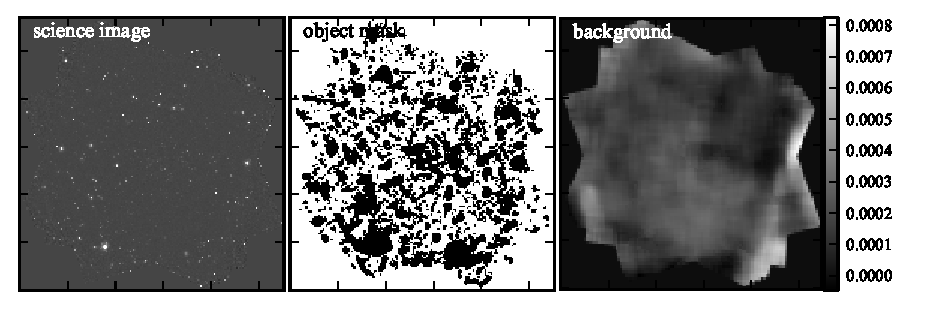
\includegraphics{figures/clrate/images_A.eps}
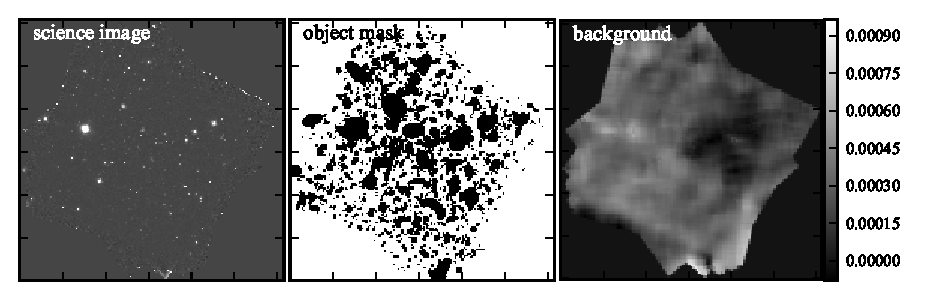
\includegraphics{figures/clrate/images_B.eps}
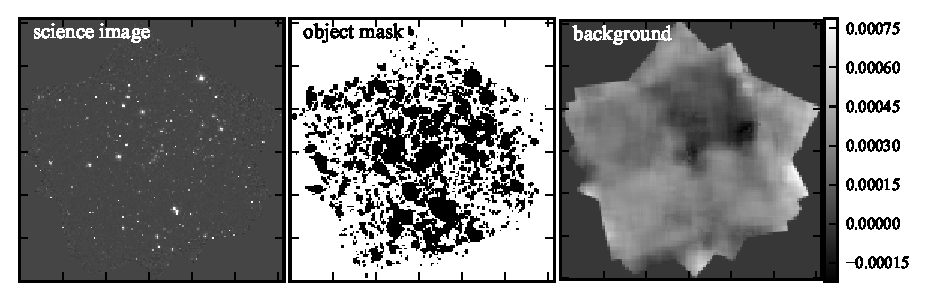
\includegraphics{figures/clrate/images_C.eps}
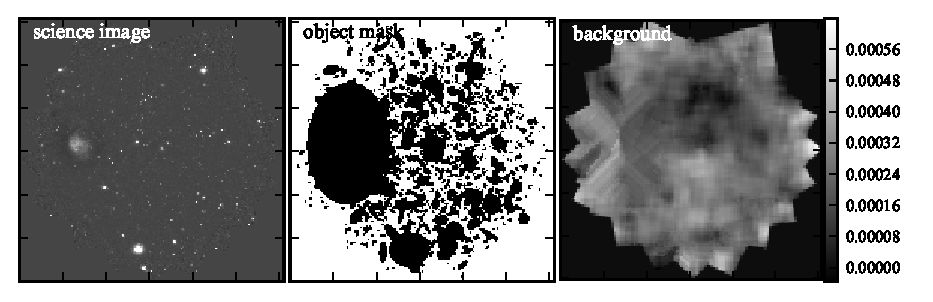
\includegraphics{figures/clrate/images_E.eps}
\end{center}
\caption[Image background determination examples]{Examples of background
  determination for the $z_{850}$ image of clusters A, B, C and E
  (descending by row). The columns are the science image (left),
  object mask (center), and derived image background (right). The
  scale is counts~s$^{-1}$~pixel$^{-1}$ in the background
  image.\label{fig:background}}
\end{figure}

In Fig.~\ref{fig:background} (right column) one can see that the
images typically have a positive flux background.  For reference,
summed over a 10 (20) pixel radius aperture a flux of 0.0005
counts~s$^{-1}$~pixel$^{-1}$ is equivalent to a flux of 0.157 (0.628)
counts~s$^{-1}$, or a $z_{850} = 26.87$ (25.37).  The other feature
that stands out is a quadrant effect. For clusters A, B and C, one
quadrant of the image has a background that is clearly lower than the
other quadrants. The effect is less obvious in clusters where the
component images had a wider range of orientations (like cluster E).

%Cluster E is an interesting case, due to the presence of a very
%extended object left of image center. {\sc SExtractor} correctly
%identifies this as a single object, resulting in a large elliptical
%region being masked. In the background image, this results in
%characteristic diagonal streaks, due to the fact that the same pixels
%are being used to compute the background at different locations in
%the masked region. This is not generally a problem though: the
%background may not be as accurate at these locations, but it should
%still be unbiased.


\subsection{Galaxy Detection and Photometry} \label{sec:lum_photometry}

For galaxy detection and photometry we use the stacked $i_{775}$ and
$z_{850}$ band images of each cluster, which have total exposure times
in the range 1060 -- 4450~seconds and 5440 -- 16,935~seconds,
respectively. 

\subsubsection{Detection}

Galaxy catalogs are created using the two-pass ``Cold/Hot'' method of
running {\sc SExtractor} first developed by \citet{rix04a} and adapted
to this survey in \citet{meyers11a}.  In the Cold/Hot method, {\sc
SExtractor} is first run in dual-image mode using the $z_{850}$ image
for detection. The detection thresholds are generally set fairly high
(Table~\ref{tab:sextractor}) in order to detect only the brighter
galaxies. The ``segmentation map'', which represents which pixels
belong to a galaxy, is saved. {\sc SExtractor} is then run again (also
in dual-image mode using the $z_{850}$ image for detection) but with
more lenient detection parameters, in order to find the fainter
galaxies. This second catalog is then cleaned by throwing out galaxies
that fall on pixels belonging to galaxies in the first catalog. The
cleaned second catalog is then combined with the first catalog.  We
remove stars from the catalog based on the CLASS\_STAR and
FLUX\_RADIUS parameters from the $z_{850}$ image.

For consistency with \citet{meyers11a}, objects are detected using the
stacked $z_{850}$ images prior to background subtraction. However,
photometry for both $z_{850}$ and $z_{775}$ is done on the background
subtracted images. Thus, for the photometry image in dual-image mode,
the {\sc SExtractor} parameters BACK\_TYPE=MANUAL and BACK\_VALUE=0.0
are used.

\subsubsection{Photometry}

It is notoriously difficult to determine accurate total fluxes for
extended sources. MAGAUTO is generally thought to be {\sc
SExtractor}'s most reliable estimator of total flux, but can still be
wrong by a large amount depending on the galaxy.  MAG\_AUTO gives the
total magnitude of an object inside a flexible elliptical aperture,
with \emph{no aperture correction}. The size of the elliptical
aperture is based on the Kron radius. Although it varies from the
original definition, for the purposes of {\sc
SExtractor} \citet{bertin96a} define the Kron radius as
\begin{equation} \label{eq:kron}
R_1 = \frac{\Sigma R I(R)}{\Sigma I(R)}
\end{equation}
over the two-dimensional aperture. The elliptical aperture used has a
semi-minor axis length $KR_1$ where the user can chose the Kron factor
$K$. Theoretically, an aperture with, for example, $K=2$ will enclose
approximately 90\% of the light of a galaxy with a \citet{sersic68a}
profile, nearly independent of its S{\'e}rsic index of the
galaxy \citep{graham05a}.

On real images with noise, things are more complicated. Because the
outskirts of the galaxy are in the noise, {\sc SExtractor} will only
assign pixels in the inner part of a galaxy to each galaxy, and only
these pixels will be counted in determining $R_1$. As a result, $R_1$
is underestimated. The amount by which it is underestimated depends on
the S{\'e}rsic index of the galaxy and its surface brightness with
respect to the background noise. As a result, the fraction of light
that an actual MAG\_AUTO aperture encloses depends on the all above
factors. In order to use MAG\_AUTO magnitudes as an accurate estimate
of total light, we must find the aperture correction empirically for
our data. We do this using the Monte Carlo simulation described below.

In order to make the aperture correction as small as possible, we use
a relatively large Kron factor of 5.0 in our MAG\_AUTO
photometry. MAG\_AUTO is only used to determine $z_{850}$ magnitudes;
$i_{775}-z_{850}$ colors are determined using PSF matching and a
smaller aperture in \citet{meyers11a}.



\subsection{Galaxy Detection Completeness and Magnitude Bias}
\label{sec:lum_correction}


To count all the flux in all cluster galaxies, we must make two
corrections: (1) add the galaxy light outside of the MAG\_AUTO
aperture, and (2) add the luminosity of all cluster galaxies below the
detection threshold of our galaxy catalog. We use a Monte Carlo
simulation of galaxies placed on the real survey data to determine
both the detection efficiency as a function of galaxy magnitude, and
the fraction of galaxy light inside the MAG\_AUTO aperture. 

\subsubsection{Galaxy Monte Carlo Simulation}

Each simulated galaxy has an elliptical S{\'e}rsic profile
given by
\begin{equation}
r = \sqrt{x^2 + (y/q)^2}
\end{equation}
\begin{equation}
\Sigma(r) = \Sigma_e e^{-\kappa [(r/r_e)^{1/n}-1]}
\end{equation}
where $\kappa$ is coupled to $n$ such that half the total flux is
always within $r_e$. For $n \gtrsim 2$, $\kappa \approx 2n - 0.331$;
at low $n$, $\kappa(n)$ flattens out toward 0, and is obtained by
interpolation. Here we use the approximation $\kappa(n)=1.7233
n^{1.0902}$ for $0<n<2$ and $\kappa = 2n -0.331$ for $n>2$. The total
flux is given by
\begin{equation}
F_{\rm tot} = 2\pi r_e^2 \Sigma_e e^\kappa n \kappa^{-2n} \Gamma(2n)q
\end{equation}
\newpage

%%%%%%%%%%%%%%%%%%%%%%%%%%%%%%%%%%%%%%%%%%%%%%%%%%
% FIGURE: ONE SIMULATED GALAXY                   %
%%%%%%%%%%%%%%%%%%%%%%%%%%%%%%%%%%%%%%%%%%%%%%%%%%
\begin{SCfigure}[0.7][tp]
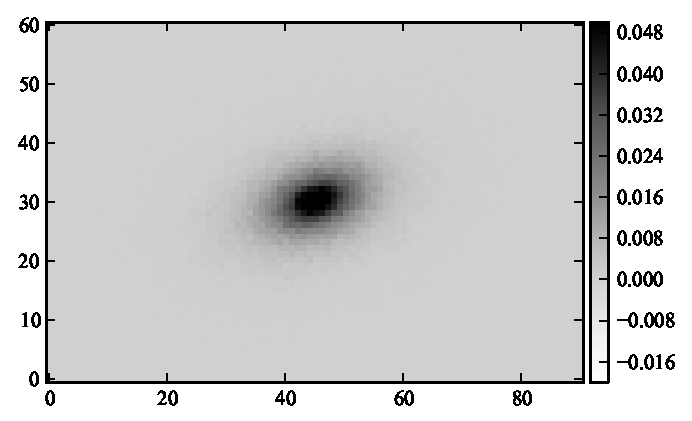
\includegraphics[width=0.65\textwidth]{figures/clrate/onesimgal.eps}
\caption[Example of a simulated galaxy]{Example of a simulated galaxy
with S{\'e}rsic index $n=1$, ellipticity $q=0.6$, magnitude $z_{850} =
  22.5$, and effective radius $r_e = 9$ pixels. Poisson noise is
  included but background noise has not been
  added. \label{fig:onesimgal}}
\end{SCfigure}

%%%%%%%%%%%%%%%%%%%%%%%%%%%%%%%%%%%%%%%%%%%%%%%%%%
% FIGURE: R_E OF SPECTROSCOPIC REDSHIFT GALAXIES %
%%%%%%%%%%%%%%%%%%%%%%%%%%%%%%%%%%%%%%%%%%%%%%%%%%
\begin{figure}[hp]
\begin{center}
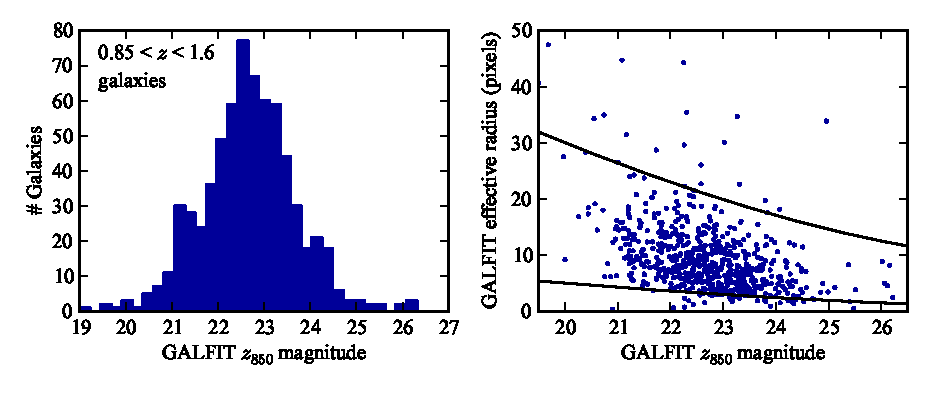
\includegraphics{figures/clrate/specgals.eps}
\end{center}
\caption[Effective radii of spectroscopically-confirmed galaxies]{{\it
    Left panel:} The distribution of GALFIT $z_{850}$ magnitudes for
  the 672 galaxies with spectroscopic redshifts $0.85 < z < 1.6$.
  {\it Right panel:} The GALFIT effective radius $r_e$ as a function
  of magnitude for the same galaxies. The black lines show the range
  of effective radius used in the Monte Carlo. Given a simulated
  galaxy magnitude, an effective radius is randomly selected from a
  flat distribution between the lower and upper black lines.
  \label{fig:specgals}}
\end{figure}

\noindent where $\Gamma(2n)$ is the gamma function. The
simulated galaxy is convolved with a (very rough) $3 \times 3$ PSF and
Poisson noise is added.  Each galaxy is simulated out to a radius of $5r_e$. 
An example of a simulated galaxy is shown in Figure~\ref{fig:onesimgal}.

The S{\'e}rsic index $n$ is simply selected from a flat distribution
ranging from $n = 0.7$ to $n = 4.5$, and the minor to major axis ratio
$q$ selected from a flat distribution ranging from $q = 0.3$ to $q =
1$.  The distribution of galaxy angular sizes $r_e$ will also affect the
results. For guidance on the size of the galaxies of concern (namely,
those at $z \gtrsim 0.9$) we turned to the 672 galaxies in the survey
with spectroscopic redshifts in the range $0.85<z<1.6$. These 672
galaxies were all fit with {\sc galfit} \citep{peng02a}, which fits a
value for $r_e$.  Figure~\ref{fig:specgals} (left panel) shows the
distribution of $r_e$ and total magnitude for these galaxies. Based on
this distribution (and considering that dimmer galaxies and those with
larger effective radii are selected against), we chose a range of
effective radius that depends on the magnitude, shown in
Fig.~\ref{fig:specgals}, left panel, between the two black
lines. Given a magnitude, a galaxy's effective radius is chosen from a
uniform distribution of $r_e$ in the range shown.

\begin{figure}[t]
\begin{center}
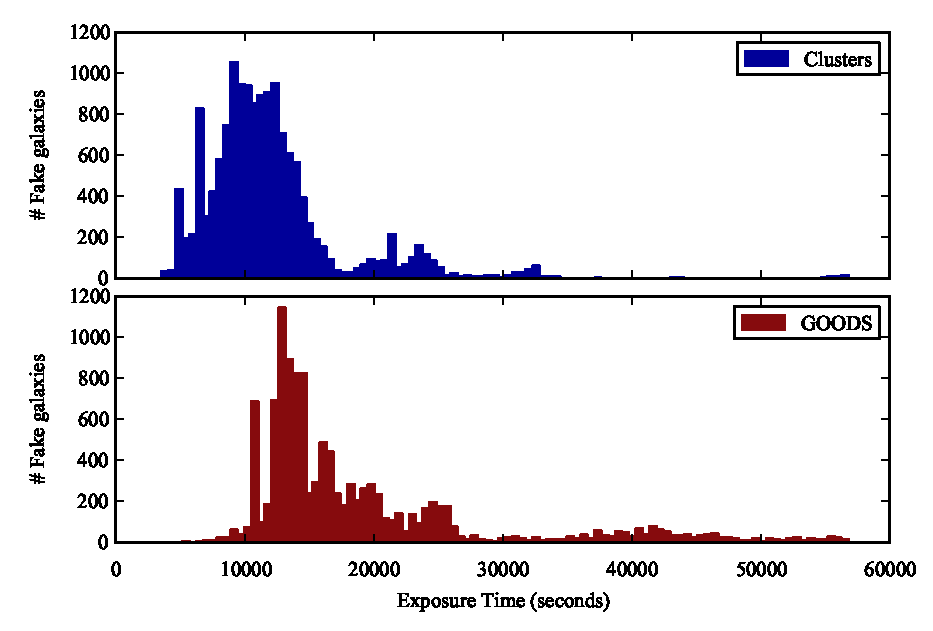
\includegraphics{figures/clrate/fakegals_exptime.eps}
\end{center}
\caption[Image depths at location of simulated galaxies]{The
  distribution of image depths (in effective exposure time) at the
  location of simulated galaxies. {\it Top panel:} A total of 15,000
  simulated galaxies were placed on cluster images. {\it Bottom
    panel:} A total of 12,000 simulated galaxies were placed on GOODS
  images. 304 galaxies were placed on the HUDF which has an effective
  exposure time of approximately 350,000 seconds, and are thus not
  shown.\label{fig:exptime}}
\end{figure}

To avoid overcrowding the images, only 200 galaxies are placed on each
image. Galaxies are only placed on the same regions of the images used
in the cluster luminosity analysis. For the GOODS fields, this is
selected circular regions with radii 1.4~arcminutes. For the cluster
fields, only regions with effective exposure time above a certain
threshold are used. This effectively eliminates the outskirts of each
field, leaving a region with mostly uniform depth for each
cluster. The distribution of effective exposure times at the location
of the simulated galaxies is shown in Fig.~\ref{fig:exptime} for all
galaxies placed on cluster fields (top panel) and all galaxies placed
on GOODS fields (bottom panel). Additionally, we enforce a minimum
separation of 10 pixels between the center of a simulated galaxy and
the center of any existing galaxy (and a minimum separation of 100
pixels from the center of any existing galaxy brighter than
$z_{850} \sim 21$). This ensures that the simulated galaxies will not
be confused with existing galaxies and the output catalog will be
cleanly comparable with the input catalog. A total of 15,000 and
12,000 galaxies were simulated on cluster fields and GOODS fields
respectively.

Images with simulated galaxies added are then run through the
background-subtraction and catalog-extraction pipelines. The resulting
catalog for each image is then compared to the input galaxies. The
closest detected galaxy within 5 pixels of a simulated galaxy is
matched to the simulated galaxy. If no galaxy is detected within 5
pixels of a simulated galaxy, the galaxy is counted as not having been
found by {\sc SExtractor}. 

\subsubsection{Galaxy Detection Efficiency}

%%%%%%%%%%%%%%%%%%%%%%%%%%%%%%%%%%%%%%%
% FIGURE: GALAXY DETECTION EFFICIENCY %
%%%%%%%%%%%%%%%%%%%%%%%%%%%%%%%%%%%%%%%
\begin{figure}[tp]
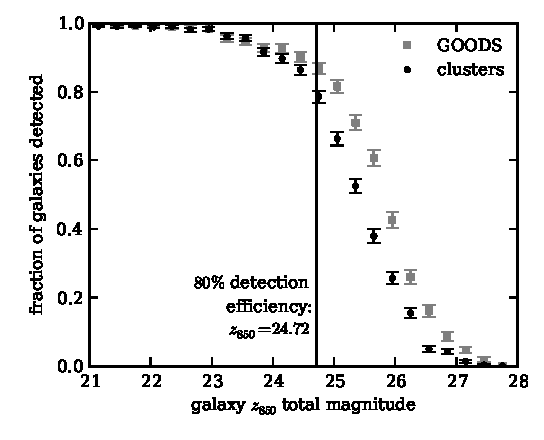
\includegraphics[width=0.5\textwidth]{figures/clrate/fakegals_eff.eps}
\includegraphics[width=0.5\textwidth]{figures/clrate/fakegals_eff_exptime.eps}
\caption[Simulated galaxy detection efficiency]{{\it Left panel:} Percentage of simulated 
galaxies recovered by {\sc SExtractor} as a function of total galaxy
  $z_{850}$ magnitude for simulated galaxies placed on cluster fields
  (black circles) and GOODS fields (grey squares). The
  detection efficiency drops to 80\% at $z_{850} = 24.72$ for cluster
  fields (vertical line). We discard all galaxies dimmer than
  this value.  {\it Right panel:} The variation in detection
  efficiency with exposure time, for cluster fields only.  There are
  2654, 4877, and 7469 galaxies in the three bins in order of
  increasing image depth. The corresponding 80\% recovery magnitudes
  are 24.76, 25.33, and 25.48 (AB). The differences in detection
  efficiency are small, particularly above the $z_{850}$ = 24.72 (Vega) =
  25.26 (AB) magnitude cutoff.
\label{fig:fakegals_eff}}
\end{figure}

The detection efficiency as a function of galaxy magnitude is shown in
Figure~\ref{fig:fakegals_eff}. For the average of all cluster fields,
the detection efficiency drops to 80\% at $z_{850} = 24.72$. We use
this magnitude as a cutoff in our selection, discarding all galaxies
dimmer than this magnitude.  We later correct total cluster
luminosities for the uncounted light from these galaxies by using an
assumed cluster luminosity function.  In reality, the detection
efficiency varies slightly from field to field (and even within a
field) due to exposure time variations (Fig.~\ref{fig:fakegals_eff},
right panel, shows the variation in detection efficiency with exposure
time for cluster fields). However, to first order the variation is
accounted for by using the average efficiency in all fields. In
addition, the total luminosity of $z_{850} > 24.72$ cluster galaxies
is small (as shown below), so slight changes in the cutoff will have a
negligible effect on the total luminosity.

\subsubsection{MAG\_AUTO Aperture Correction}

%%%%%%%%%%%%%%%%%%%%%%%%%%%%%%%%%%%%%%%%%%%%%%%%%%%%%%%%%%%%%%%%%%
% PLOT: GALAXY MAG_AUTO CORRECTION : PAGE GRID of N vs Delta Mag %
%%%%%%%%%%%%%%%%%%%%%%%%%%%%%%%%%%%%%%%%%%%%%%%%%%%%%%%%%%%%%%%%%%
\begin{figure}[tp]
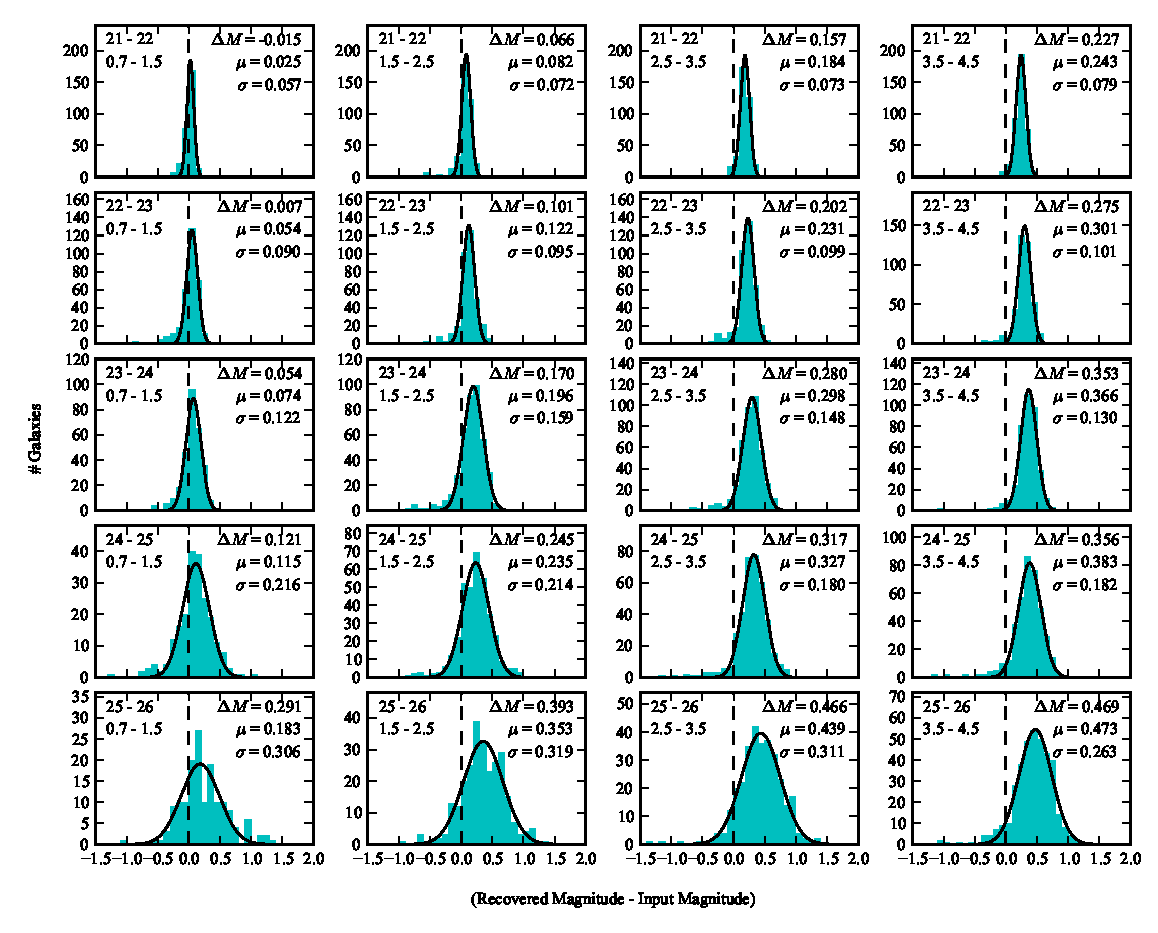
\includegraphics[angle=270]{figures/clrate/fakegals_grid_n.eps}
\caption[Aperture correction as a function of magnitude and S{\'e}rsic
index $n$]{The distribution of aperture corrections as a function of
magnitude and S{\'e}rsic index $n$. The range of magnitudes and
S{\'e}rsic indices included in each panel is given in the upper left
of the panel. $\Delta M$ is the magnitude correction derived from
ratio of the total flux extracted to the total flux input. $\mu$ and
$\sigma$ describe the Gaussian fit to each distribution. 
\label{fig:fakegals_grid_n}}
\end{figure}

The fraction of galaxy light falling inside the MAG\_AUTO aperture
will depend on several parameters of the galaxy, including the galaxy
magnitude, and S{\'e}rsic index $n$. To see the dependence on
magnitude and $n$, in Figure~\ref{fig:fakegals_grid_n} we split the
simulated galaxies into bins in magnitude and $n$. For the galaxies in
each bin, we plot the distribution of the difference between the true
total magnitude and the MAG\_AUTO magnitude.  A Gaussian fit, and its
$\mu$ and $\sigma$ parameters, are shown for reference. As expected,
the distributions are wider for fainter magnitudes (descending rows in
the figure) due to increasing photometric error. The distributions
have somewhat non-Gaussian tails, particularly on the negative side. On
the negative side, this is most likely due to collisions with other
galaxies, where flux from a nearby galaxy falls in the aperture. Also
as expected, the offset grows larger with both increasing $n$ and
increasing magnitude. As $n$ or magnitude increases, the outskirts of
the galaxy are increasingly buried in noise, causing {\sc SExtractor}
to underestimate the Kron radius, leading to a smaller MAG\_AUTO
aperture.  For each distribution, $\Delta M$ is the magnitude
correction one would need to make to each galaxy in order for
the \emph{total} output flux to match the \emph{total} input
flux. Aperture corrections are based on $\Delta M$ in each bin, and
thus take into account the non-Gaussian tails in the distributions.


%%%%%%%%%%%%%%%%%%%%%%%%%%%%%%%%%%%%
% PLOT: GALAXY MAG_AUTO CORRECTION %
%%%%%%%%%%%%%%%%%%%%%%%%%%%%%%%%%%%%
\begin{SCfigure}[0.7][tb]
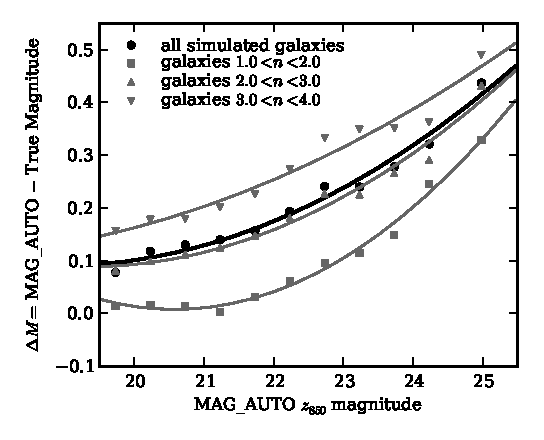
\includegraphics[width=0.6\textwidth]{figures/clrate/fakegals_apcorr.eps}
\caption[Aperture correction as a function of magnitude]{Galaxy 
MAG\_AUTO aperture correction as a function of galaxy magnitude. The
black circles show the average correction for the full distribution of
galaxies simulated, including all S{\'e}rsic indices $n$. The black
line is a fit to these points and is the relation we use. Note that it
is not extrapolated beyond the range shown. To illustrate the effect
of $n$ on the aperture correction, we plot the aperture correction for
subsets of galaxies with different S{\'e}rsic indices (Grey
squares and triangles). Galaxies with larger S{\'e}rsic indices have
a larger aperture correction.
\label{fig:fakegals_apcorr}}
\end{SCfigure}

We derive a relation between $\Delta M$ and the galaxy brightness
(Fig.~\ref{fig:fakegals_apcorr}, black circles), summing over all
$n$. We find that the relation is well-fit by a second-order
polynomial (Fig.~\ref{fig:fakegals_apcorr}, thick black line), given
by
\begin{equation}
\Delta M = 0.238 + 0.081(M_{MAG\_AUTO}-23) + 0.009(M_{MAG\_AUTO} -23)^2.
\end{equation}
%\begin{eqnarray}
%\Delta M & = & 0.238 + 0.081(M_{MAG\_AUTO}-23) + \nonumber \\
%         &   & + 0.009(M_{MAG\_AUTO} -23)^2.
%\end{eqnarray}
We use this to correct the magnitude of each detected galaxy. Note
that the correction is not extrapolated beyond the fitted range shown.

Because we cannot reliably determine $r_e$ or the S{\'e}rsic index $n$
for each galaxy, we rely on the simulated distribution of $r_e$ and
$n$ to accurately represent the true distributions. (The black circles
in Fig.~\ref{fig:fakegals_apcorr} include all simulated galaxies.)  We
have based our distribution of $r_e$ on actual galaxies, but $n$ is
less well-known. To estimate the effect of varying the $n$
distribution, we show $\Delta M$ for subsets of the simulated
galaxies, divided by S{\'e}rsic index (Fig.~\ref{fig:fakegals_apcorr},
grey points and lines).  If, instead of the flat $1<n<4$ distribution
used, all galaxies had $1<n<2$, the aperture correction would be lower
by approximately 0.10~magnitudes. If instead all galaxies had
$3<n<4$, the correction would be higher by approximately
$0.07$~magnitudes. We use $0.07$~mag as the systematic uncertainty in
the aperture correction. (All systematic uncertainties are summarized
in \S\ref{sec:clrate_results_sys} and Table~\ref{tab:clrate_sys}.)

\vspace{1in}


\subsection{$K$-Corrections} \label{sec:lum_kcorr}

We use a $K$-correction based on the BC03 stellar population spectral
models to convert the observed $z_{850}$ magnitude to a rest-frame $B$
magnitude for each cluster. The BC03 models consist of galaxy spectra
for an instantaneous starburst (``simple stellar population'', or SSP)
with various initial metallicities ($0.0001 < Z < 0.1$) and ages
($1 \times 10^5$ -- $2 \times 10^{10}$ yr). BC03 contains models for
several different stellar evolution prescriptions, and two initial
mass functions (IMF). We use the recommended Padova 1994 stellar
evolution prescription and Chabrier IMF. Figure~\ref{fig:bc03spectra}
shows examples of BC03 spectra for metallicity $Z=0.02$ at a range of
ages. Also shown are the rest-frame $U$ and $B$ bands, as well as the
observed $i_{775}$ and $z_{850}$ bands at the minimum ($0.91$) and
maximum ($1.50$) redshift of clusters in the sample. The $z_{850}$
filter is a good match to rest-frame $B$ band across much of the
redshift range of the clusters. It is the best match at $z \approx
1.07$ and shifts progressively bluer than $B$ at higher redshifts,
approximately matching $U$ at the high-redshift end of the sample.

\begin{figure}[t]
\begin{center}
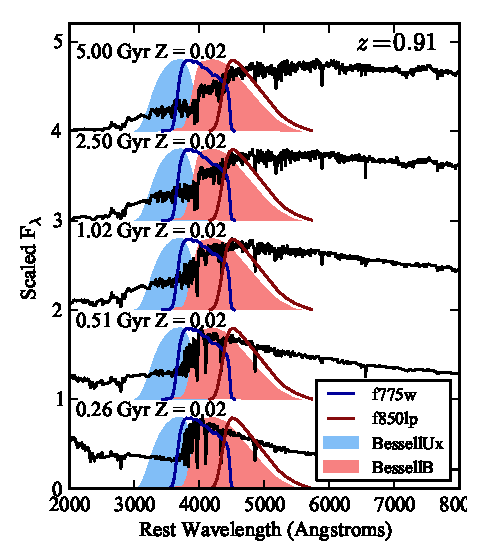
\includegraphics{figures/clrate/bc03spectra_lowz.eps}%
\includegraphics{figures/clrate/bc03spectra_highz.eps}
\end{center}
\caption[Examples of Bruzual \& Charlot (2003) spectra]{Examples
of BC03 spectra for a single initial metallicity ($Z =
0.02$) and a range of ages. The left and right panels are identical,
except that the \emph{left panel} shows the observed filters at $z=0.91$ and
the \emph{right panel} shows them at $z=1.50$ (the approximate range
of cluster redshifts).\label{fig:bc03spectra}}
\end{figure}

Rather than using a single $K$-correction for all the light in each
cluster, we apply a $K$-correction to each galaxy magnitude based on
its $i_{775}-z_{850}$ color. For each cluster's redshift, we determine
the relation between $K$-correction ($M_B$ (rest) $- z_{850}$) and
$i_{775}-z_{850}$ color, using BC03 spectra with initial metallicities
in the range $0.004 < Z < 0.05$ and ages in the range $1 \times 10^8 -
5 \times 10^9$~yr. This relation is shown for four example cluster
redshifts in Figure~\ref{fig:kcorr} (left panels). The colored lines
in each panel represent BC03 spectra with constant metallicity and age
increasing from $1 \times 10^8$ -- $5 \times 10^9$ yr.  For most
cluster redshifts in our sample, all of the spectra over this wide
range fall along the same line in $K$-correction versus color, meaning
that the color determines the $K$-correction, regardless of the
metallicity or age assumed. At $z=1.07$, where the best match between
$z_{850}$ and rest-frame $B$ is obtained, the $K$-correction is nearly
independent of color or model, as one would expect. In the redshift
range $1.15 \lesssim z \lesssim 1.4$, the curves are multi-valued for
a range of observed colors, and are the most dispersed at $z \approx
1.26$ (shown in Figure~\ref{fig:kcorr}). To select a $K$-correction
given an observed galaxy color, we average the $K$-correction for all
models with similar colors, arriving at the black line shown in each
panel.

\begin{figure}[p]
\begin{center}
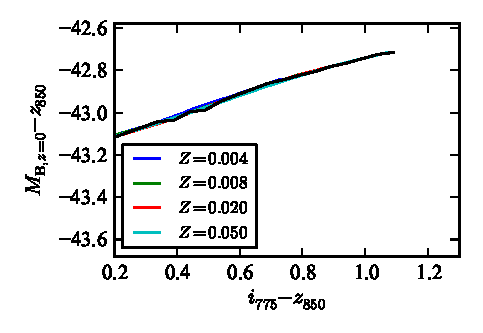
\includegraphics[width=0.45\textwidth]{figures/clrate/kcorr_mag_z1.eps}%
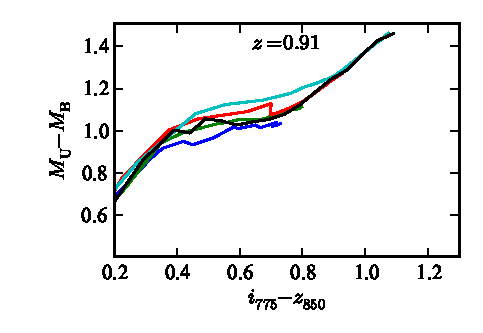
\includegraphics[width=0.45\textwidth]{figures/clrate/kcorr_color_z1.eps}
\includegraphics[width=0.45\textwidth]{figures/clrate/kcorr_mag_z2.eps}%
\includegraphics[width=0.45\textwidth]{figures/clrate/kcorr_color_z2.eps}
\includegraphics[width=0.45\textwidth]{figures/clrate/kcorr_mag_z3.eps}%
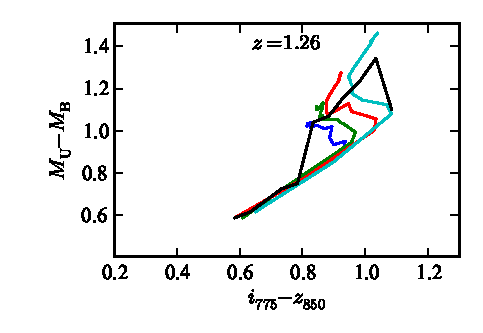
\includegraphics[width=0.45\textwidth]{figures/clrate/kcorr_color_z3.eps}
\includegraphics[width=0.45\textwidth]{figures/clrate/kcorr_mag_z4.eps}%
\includegraphics[width=0.45\textwidth]{figures/clrate/kcorr_color_z4.eps}
\end{center}
\caption[$K$-correction fits to Bruzual \& Charlot (2003)
spectra]{$K$-correction fits, based on BC03 spectra.  The colored
lines in each panel represent BC03 spectra with constant initial
metallicity and age increasing from $1 \times 10^8$ -- $5 \times 10^9$
yr. The black line is the relation used in this analysis. The \emph{left
panels} show the $K$-correction as a function of observed galaxy color
and the \emph{right panels} show the rest-frame $U-B$ color as a function of
observed color. \label{fig:kcorr}}
\end{figure}

The dispersion of the models about the best-fit line is $<0.03$~mag at
redshifts $\lesssim 1.1$ and $\gtrsim 1.4$, and reaches its largest
value of 0.09~mag at $z=1.26$. We calculate the $K$-correction for
each galaxy using this best-fit relation, effectively assuming that
every galaxy is at the cluster redshift. This results in an incorrect
luminosity for non-cluster member galaxies, but this is accounted for
by performing the same $K$-correction on the galaxies in the GOODS
fields prior to subtracting their luminosity. 


\vspace{1.2in}


% From draft:

%For all remaining galaxies, I convert the observed $z_{850}$
%magnitude into an absolute rest-frame $B$ magnitude, {\it assuming}
%the galaxy is at the cluster redshift. (Of course, this will not give
%an accurate $B$ magnitude for galaxies not in the cluster, but
%following the same procedure for the ``background'' fields will mean
%that the correct magnitude is subtracted.) To make this
%$K$-correction, I use the stellar population synthesis models
%of BC03.


%In computing the $K$-correction for each cluster, I consider spectra
%with initial metallicity 0.004, 0.008, 0.02, and 0.05, and in the age
%range $1 \times 10^8$ -- $5 \times 10^9$ yr. For each spectrum in this
%range, I compute the $i_{775} - z_{850}$ color (with the spectrum
%redshifted to the cluster redshift), the $U - B$ rest-frame color, and
%$M_{B,z=0}-z_{850}$, which is the difference between the observed
%$z_{850}$ magnitude and the absolute rest-frame $B$ magnitude
%(assuming the spectrum is at the cluster redshift). Plotting
%$M_{B,z=0}-z_{850}$ against $i_{775} - z_{850}$ gives the
%$K$-correction as a function of the observed galaxy color.


%This line is used to convert the
%observed $z_{850}$ magnitude to a rest-frame absolute $B$ magnitude
%for each galaxy, given its color. The standard deviation of the
%residuals of the models from this best fit line are 0.004, 0.004,
%0.094, and 0.024 magnitudes, for redshifts 0.91, 1.07, 1.26 and 1.45,
%respectively. Thus, for most clusters, we expect the error associated
%with the $K$-correction to be quite negligible (less than 3\%), and
%even in the worst cases, should generally be below 10\%. For galaxies
%with colors outside the range of models, the model with the nearest
%color is used to $K$-correct, in order to avoid errors from
%extrapolating the fit far beyond the fitted range. Because galaxies
%with these extreme colors are most likely not part of the cluster, any
%errors will cancel out when the background is subtracted. In the right
%panels of Figure~\ref{fig:kcorr} the rest-frame $U-B$ color is shown
%as a function of observed color, exhibiting similar
%characteristics. The standard deviation of residuals for color are
%0.030, 0.010, 0.106, and 0.025 magnitudes, for redshifts 0.91, 1.07,
%1.26 and 1.45, respectively.


\subsection{Luminosity Function Correction} \label{sec:lum_faintgals}

We estimate the total luminosity of all galaxies below the detection
limit of $z_{850} = 24.72$ using a \citet{schechter76a}
luminosity function, which gives the number of galaxies in the
luminosity interval $[L,L+dL]$ in a given sample,
\begin{equation}
\Phi(L)dL = \Phi^\ast (L/L^\ast)^\alpha e^{-L/L^\ast} d(L/L^\ast).
\end{equation}
$\Phi^\ast$ is a normalization, $L^\ast$ is a
characteristic galaxy luminosity, and $\alpha$ is a unit-less
constant. The ratio of total to observed luminosity is then
\begin{equation}
C = \frac{\int_0^\infty L\Phi(L)dL}{\int_{L_{lim}}^\infty L\Phi(L)dL},
\end{equation}
and we multiply each observed cluster luminosity by C to get the total
luminosity. 

We assume values for $L^\ast$ and $\alpha$ determined in other studies
and use our data to perform a rough consistency check. For $\alpha$,
studies have shown that the value does not evolve much from low
redshift, at least for redder galaxies. Analyzing only red galaxies in
28 clusters spanning $0 < z < 1.3$, \citet{andreon08a} find $\alpha =
-0.91 \pm 0.06$ (rest-frame $V$-band) with no discernible trend in
redshift \citep[see also][]{andreon06a,andreon06c}. From five
intermediate-redshift clusters ($0.54<z<0.9$), \citet{crawford09a}
find a somewhat flatter faint-end slope $\alpha \sim -0.6$ (rest-frame
$B$-band) for the red-sequence luminosity function. Looking at the
full luminosity function, \citet{goto05a} find $\alpha = -0.82 \pm
0.10$ in one cluster at $z=0.83$ (rest-frame $B$-band), compared to
$\alpha = -1.00 \pm 0.06$ in 204 low-redshift clusters (rest-frame
$g$-band) \citep{goto02a}. In redder bands, \citet{strazzullo06a} find
$\alpha \sim -1$ for three clusters at redshifts $1.11 < z < 1.27$ (in
approximately rest-frame $z$ band). Summarizing, most studies find a
value consistent with $\alpha \sim -0.9$, and we assume this value in
computing $C$.

%Note that for the majority of our clusters, the observed $z_{850}$
%band corresponds more closely to rest-frame $B$-band than rest-frame
%$U$ band, but that for the highest-redshift clusters in our sample, we
%are observing rest-frame $U$ band. \citet{goto02a} and \citet{goto05a}
%find a steeper faint-end slope ($\alpha \sim -1.3$) in rest-frame $U$
%band for the full cluster luminosity function, due to the dominance of
%blue star-forming galaxies in the UV. There is little evidence of a
%pass-band dependence for the redder
%galaxies \citep[e.g.,][]{goto02a,andreon06b}.  As we are more
%concerned with tracing the light of redder galaxies that dominate the
%cluster stellar mass, we use a constant value of $\alpha = -0.9$
%independent of cluster redshift.

Values for $M^\ast$ are also reported in most of the above-mentioned
studies. Studies of red galaxies find that the variation of $M^\ast$
with redshift is consistent with passive evolution, with $M^\ast$
decreasing towards higher
redshifts \citep{andreon06c,crawford09a}. \citet{crawford09a} find
$M^\ast_B = -21.1$ and $M^\ast_B \sim -21.3$ (with errors of
approximately a half magnitude) for two clusters at redshifts 0.75 and
0.83. $K$-correcting from the observed
$[3.6]$-band, \citet{andreon06c} find $M^\ast_B \sim -21.7$ at $z \sim
1.1$, with approximately 0.5~magnitudes of evolution between $z=0.3$
and $z=1.1$. At lower redshift (considering all
galaxies) \citet{goto02a} find $M^\ast_B \sim -21.6$, compared to
$M^\ast_B \sim -21.0$ for one cluster at $z=0.83$ \citep{goto05a}. On
the basis of these measurements, we assume a value of $M^\ast_B =
-21.7$.

We have checked our assumed $M^\ast_B$ and $\alpha$ for consistency
with our data. With the set of spectroscopically-confirmed cluster
galaxies from our clusters at $z<1.2$, we confirmed that the bright
end of the luminosity function is consistent with $M^\ast_B = -21.7$,
and strongly inconsistent with values outside the range $M^\ast_B =
-21.7 \pm 0.5$. We also determined the luminosity function using a
statistical subtraction of the ``background'' luminosity function from
the GOODS fields (Fig.~\ref{fig:galproperties_lumfunc}), finding
excellent agreement with the assumed $M^\ast_B$ and $\alpha$ values
over the range $-24 < M_B < -19.8$. ($M_B = -19.8$ corresponds to the
detection limit in the highest-redshift clusters.)

%%%%%%%%%%%%%%%%%%%%%%%%%%%%%%%%%%%%%%%
% FIGURE: CLUSTER LUMINOSITY FUNCTION %
%%%%%%%%%%%%%%%%%%%%%%%%%%%%%%%%%%%%%%%
\begin{figure}[tb]
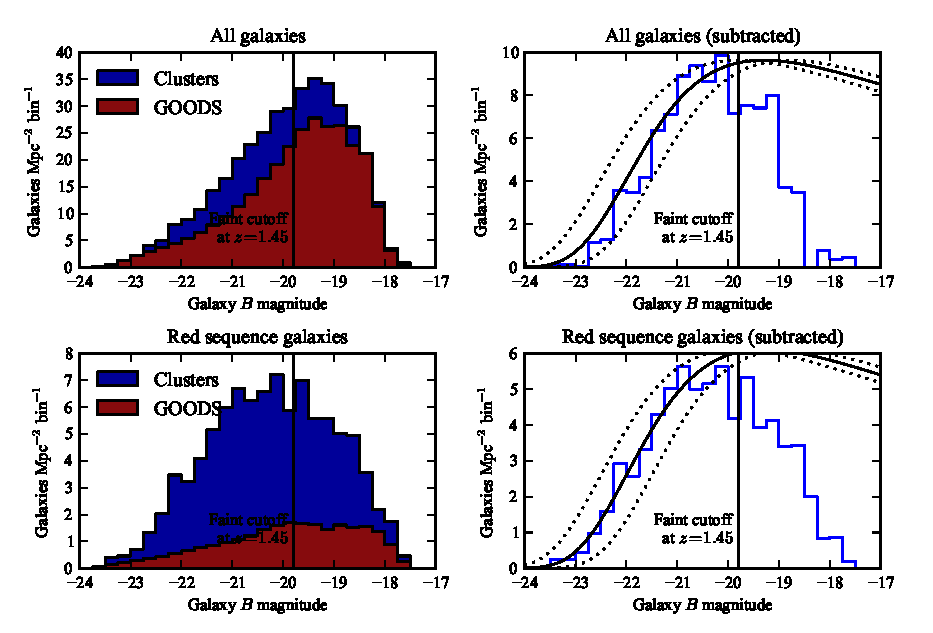
\includegraphics[width=\textwidth]{figures/clrate/galproperties_lumfunc.eps}
\caption[Luminosity function of cluster galaxies]{The luminosity 
function of cluster galaxies (\emph{top panels}) and red-sequence-only
galaxies (\emph{bottom panels}). The \emph{left panels} show the luminosity function
in cluster fields and GOODS fields, showing the clear overdensity in
the cluster fields relative to GOODS. The \emph{right panels} show the
distribution after subtracting the GOODS distribution. The black solid
line shows the luminosity function we assume here ($M^\ast_B = -21.7$,
$\alpha=-0.9$) with dotted lines showing the range used to asses the
systematic uncertainty ($M^\ast_B = -21.7 \pm 0.5$). These
distributions are only reliable to the left of the vertical solid
line, which represents the detection limit in the highest-redshift
cluster.\label{fig:galproperties_lumfunc}}
\end{figure}

For each cluster, we calculate $C$ in the observer frame, converting
$M^\ast_B = -21.7$ to the observed $z_{850}$ band, using the cluster
redshift and a $K$-correction based on a passive galaxy template. In
Table~\ref{tab:lum_params} we report the value $z_{850}^\ast$ and the
resulting correction $C$ for each cluster. The correction is less than
$5\%$ for the majority of clusters, rising to a maximum of 14\% for
the highest-redshift cluster. Because the correction is so small,
varying the assumed values of $M^\ast_B$ and $\alpha$ does not have a
large effect on the total luminosity. Varying $M^\ast_B$ by $\pm
0.5$~mag (a larger range than that allowed by our data) changes the
average correction by only $^{+4}_{-2}\%$. Varying $\alpha$ by $\pm
0.2$ changes the average correction by $^{+5}_{-2}\%$. We
conservatively take $^{+10}_{-3}\%$ (the full range when varying both
concurrently) as the systematic uncertainty in luminosity from the
faint-end correction (summarized in \S\ref{sec:clrate_results_sys}).

%%%%%%%%%%%%%%%%%%%%%%%%%%%%%%%
% luminosity parameters table %
%%%%%%%%%%%%%%%%%%%%%%%%%%%%%%%
\begin{table}[t]
\begin{center}
\caption{\label{tab:lum_params} Bright cutoff magnitudes 
and luminosity function parameters}
\vspace{10pt}
\begin{footnotesizetabular}{lccccc}
\hline
\hline
ID & $z$ & Cutoff from & $z_{850}^{\rm bright}$ & $z_{850}^\ast$ & $C$\\
\hline
A & 1.46 & Max cD & $21.09$ & $22.80$ & $1.143$\\
B & 1.12 & cD & $20.11$ & $21.38$ & $1.033$\\
C & 0.97 & cD & $19.87$ & $20.79$ & $1.018$\\
D & 1.02 & BCG & $20.13$ & $20.95$ & $1.021$\\
E & 1.03 & cD & $19.40$ & $20.99$ & $1.022$\\
F & 1.11 & Max cD & $19.63$ & $21.34$ & $1.031$\\
G & 1.26 & BCG & $20.34$ & $22.04$ & $1.064$\\
H & 1.24 & BCG & $20.33$ & $21.95$ & $1.058$\\
I & 1.34 & Max cD & $20.66$ & $22.37$ & $1.092$\\
J & 1.37 & Max cD & $20.77$ & $22.50$ & $1.104$\\
K & 1.41 & Max cD & $20.92$ & $22.65$ & $1.122$\\
L & 1.37 & Max cD & $20.77$ & $22.50$ & $1.104$\\
M & 0.90 & Max cD & $18.69$ & $20.53$ & $1.014$\\
N & 1.03 & BCG & $20.22$ & $20.99$ & $1.022$\\
P & 1.1\phn & Max cD & $19.58$ & $21.29$ & $1.030$\\
Q & 0.95 & cD & $20.01$ & $20.66$ & $1.015$\\
R & 1.22 & Max cD & $20.15$ & $21.86$ & $1.054$\\
S & 1.07 & Max cD & $19.44$ & $21.16$ & $1.026$\\
T & 0.97 & Max cD & $19.00$ & $20.75$ & $1.017$\\
U & 1.04 & Max cD & $19.31$ & $21.04$ & $1.022$\\
V & 0.90 & cD & $18.89$ & $20.49$ & $1.013$\\
W & 1.26 & Max cD & $20.33$ & $22.04$ & $1.064$\\
X & 1.10 & Max cD & $19.58$ & $21.34$ & $1.031$\\
Y & 1.24 & cD & $20.29$ & $21.90$ & $1.056$\\
Z & 1.39 & cD & $20.85$ & $22.58$ & $1.112$\\
\hline
\end{footnotesizetabular}

\end{center}
{\footnotesize 
{\bf Note.} --- ``Cutoff from'' refers to how $z_{850}^{\rm bright}$ is
determined.  ``cD'': magnitude of visually central dominant
galaxy. ``BCG'': magnitude of visually classified brightest cluster
elliptical (but not central) galaxy. ``Max cD'': Cluster does not have
obvious cD galaxy or clear BCG. In this case, $z_{850}^{\rm bright}$
is $K$-corrected from $M_B = -23.42$, the absolute magnitude of the
brightest cD galaxy in the entire sample.}
\end{table}



\subsection{Determining Cluster Centers} \label{sec:lum_centers}

The 25 clusters are heterogeneous in the spatial distribution of their
member galaxies. Some clusters have very obvious cores with tens of
red elliptical galaxies, while in others no central overdensity is
obvious to the eye. For these later clusters, the exact ``center'' of
the cluster is nearly impossible to define from the ACS imaging
data. Because the luminosity analysis is not very dependent on having
an accurate center, we use a hybrid method to arrive at the cluster
positions listed in Table~\ref{tab:clusters}. For those clusters
having a clear central-dominant (cD) galaxy, the position of the cD
galaxy is used. Cluster Y has two close cD-like galaxies; the position
given is that of the Southwest galaxy, which is slightly brighter and
looks more centrally located with respect to other red elliptical
galaxies. For the 18 clusters lacking a cD galaxy we first attempt to
find a central overdensity of red-sequence galaxies by choosing the
position that maximizes the total luminosity of red sequence galaxies
within 0.1~Mpc (where a red-sequence galaxy is one that has a color
within 0.15~magnitudes of the cluster's red sequence and an
ellipticity less than 0.5). We then averaged the position of the red
sequence galaxies contained in that aperture (weighting by galaxy
luminosity) to get a slightly more refined (and unique) position. This
position is then evaluated by eye with respect to red elliptical
galaxies outside the 0.1~Mpc circle. If the position represents a
clear overdensity and seems consistent with galaxies outside the
circle, we use this position. This is done for clusters F (16
red-sequence galaxies within 0.1 Mpc), G (11), I (8), N (14), R (18),
T (19), W (16) and X (22). For clusters A (16), J (8), M (8) and S
(7), the algorithm gives a reasonable result, but the overdensity
seems offset from the larger distribution of galaxies and we chose a
(nearby) position by eye. For clusters H, K, L, O, P, U, the algorithm
either fails due to the presence of bright (lower redshift)
red-sequence interlopers in the field, or because there is no clear
overdensity of galaxies. For these clusters the center chose by eye is
less reliable.



\subsection{``Background'' Luminosity} \label{sec:lum_goods}


For each cluster we sum the $K$-corrected $B$-band luminosity of all
galaxies brighter than the detection limit $z_{850} = 24.72$.  To
reduce noise, we discard galaxies that are clearly too bright to be
cluster members. In clusters with a central dominant (cD) galaxy or
dominant (but not central) brightest cluster galaxy(BCG), the bright
cutoff magnitude is set to the magnitude of the cD galaxy or BCG. In
clusters lacking a clearly dominant galaxy, we conservatively set the
cutoff based on the absolute magnitude of the most luminous cD galaxy
in any cluster, $M_B = -23.42$ (from cluster XMMU J2235.3$-$2557). The
bright cutoff magnitude in the observer frame, $z_{850}^{\rm bright}$,
is listed for each cluster in Table~\ref{tab:lum_params}.  Because
the bright cutoff is chosen so conservatively, we expect that no
cluster galaxies are discarded. The effect of being overly
conservative is only to add noise, and this is captured in the
statistical uncertainty described below.

For each cluster we apply the same selection criteria and
$K$-corrections to the GOODS fields to determine the ``background''
specific to that cluster. The GOODS fields
consist of a North field centered at approximately $\alpha = 12^{\rm
h} 36^{\rm m}$, $\delta = +62^{\circ} 14'$ and a South field centered
at approximately $\alpha = 3^{\rm h} 32^{\rm m}$, $\delta =
-27^{\circ} 48'$. Each field has been imaged with ACS over an area of
15 ACS tiles, or $\sim$170 arcmin$^2$. I chose these fields because
they have ACS $z_{850}$ imaging to a depth similar to, or deeper than,
the cluster fields, over a relatively wide area. Also, having two widely
separated fields (North and South) helps minimize bias from galaxy
density fluctuations.

\begin{figure}[p]
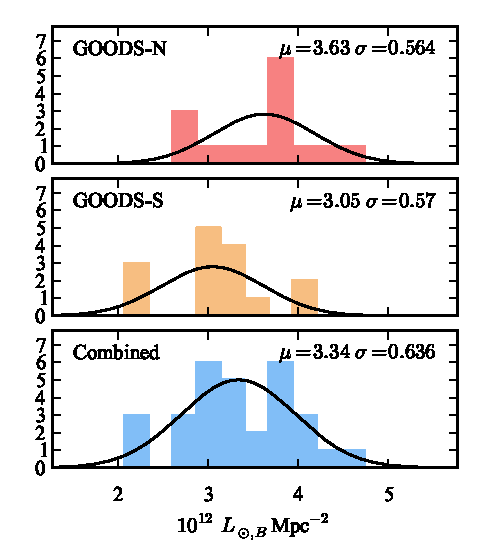
\includegraphics{figures/clrate/bkghist_all_V.eps}%
\includegraphics{figures/clrate/bkghist_all_S.eps}
\includegraphics{figures/clrate/bkghist_all_G.eps}%
\includegraphics{figures/clrate/bkghist_all_A.eps}
\caption[Distribution of luminosity density in GOODS
fields.]{Distribution of luminosity density in GOODS fields, with
galaxy selection and $K$-corrections applied for cluster V ($z=0.91$,
\emph{upper left}), cluster S ($z=1.07$, \emph{upper right}), cluster G 
($z=1.26$, \emph{lower left}), and cluster A ($z=1.45$, \emph{lower
right}). \label{fig:bkghist_all}}
\end{figure}

We select 30 non-connected circular regions (15 in each of GOODS North
and South) of radius $1'.4$, similar to the size of the cluster
fields.  ($1'.4$ corresponds to 0.654, 0.697, and 0.711 Mpc at
$z=0.9$, 1.2 and 1.5, respectively.)  The distribution of luminosity
densities in these 30 regions is shown for four example clusters in
Figure~\ref{fig:bkghist_all}. Because the same 30 regions are used for
each cluster, the resulting distributions are quite similar, though
not identical because of the different selections and $K$-corrections
used.  The average luminosity density of these fields is taken as the
``background'' luminosity for the cluster, and the standard deviation
(typically 15 -- 20 \% of the average) is taken as the error in this
background luminosity due to variations between fields.

We have implicitly assumed that the GOODS average accurately
represents the cosmic average. GOODS incorporates only two widely
separated fields. As a result, the average luminosity density may
differ from the cosmic average due to variations in large scale
structure. As a rough estimate of the cosmic variance, we compare the
two GOODS fields.  The average luminosity density of the GOODS-North
regions is consistently higher than that of the GOODS-South regions by
15 -- 20\% (Fig.~\ref{fig:bkghist_all}). This means that the ``standard deviation'' of these two
samples of large scale structure is $\sim$8\%. We checked this using
the cosmic variance calculator made available
by \citet{trenti08a}\footnote{\url{http://casa.colorado.edu/~trenti/CosmicVariance.html}}. The
expected cosmic variance in galaxy number counts in the redshift
window $0.7 < z < 1.7$ for one GOODS field is approximately $\sim$6\%,
in good agreement with our na\"ive estimate. Conservatively, we take
$8\%$ as the cosmic variance for one GOODS field. For
the \emph{average} of the North and South fields, this implies a
cosmic variance of $8\%/\sqrt{2} \sim 6\%$.

One might be additionally concerned that the ``background'' in the
cluster fields is biased higher than the cosmic average because
clusters form in regions of large-scale overdensities. However, each
cluster field is a ``pencil-beam'' galaxy survey, so the vast majority
of non-cluster galaxies will not be associated with the high-density
region in which each cluster formed.


\subsection{Cluster Luminosity Profiles} \label{sec:lum_profiles}

Ideally one would measure a two-dimensional luminosity density,
$L(x,y)$, for each cluster, as in Equation~(\ref{eq:ratedenom}).
However, the large background makes this difficult. For our purpose
(which is to account for variations in control time with radius), it
is sufficient to assume the clusters have a circularly symmetric
luminosity distribution, $L(r)$. For each cluster, we sum the total
luminosity in annuli of width 0.1~Mpc. For nearly all clusters there
is a clear overdensity relative to the background out to $r \sim
0.3$~Mpc (Fig.~\ref{fig:allprofiles_all}). Beyond $0.3$~Mpc, the
luminosity measurement is dominated by background noise for most
clusters. This might appear to be a problem; we wish to characterize
the cluster luminosities out to $r \gtrsim 0.7$~Mpc, the area over
which we searched for SNe. In fact, it is only necessary to accurately
measure the \emph{average} luminosity profile over the full area (the
denominator of Eq.~\ref{eq:rate} is the sum of the cluster
luminosities, weighted by control time). Averaging all 25 clusters,
there is a significant measurement of the luminosity profile out to
$>0.5$~Mpc (Fig.~\ref{fig:avgprofile_mult}, left panels), and the
average cluster luminosity within $r<0.6$~Mpc has an error of $12\%$
(statistical only) and $\sim 20\%$ (statistical $+$ cosmic variance),
below the Poisson error in the number of SNe detected.

%%%%%%%%%%%%%%%%%%%%%%%%%%%%%%%%%%%%%%%%%%%%%%%%%%%%%%%%%%%%%%%%%%%%
% FIGURES: LUMINOSITY PROFILES -- ALL CLUSTERS                     %
%%%%%%%%%%%%%%%%%%%%%%%%%%%%%%%%%%%%%%%%%%%%%%%%%%%%%%%%%%%%%%%%%%%%
\begin{figure}[tp]
\includegraphics[angle=270]{figures/clrate/allprofiles_all.eps}
\caption[Luminosity profiles of 25 clusters]{Luminosity profiles
of all 25 clusters. The grey line and shaded region represents the
estimated background luminosity density and uncertainty on the
background at each radius. The background uncertainty decreases
with radius because larger annuli sample more area. At large radii,
the uncertainty increases again because only some parts of the outer
annuli (on the deepest part of the image) are used in computing the
luminosity. \label{fig:allprofiles_all}}
\end{figure}

\begin{figure}[tp]
\includegraphics[angle=270]{figures/clrate/allprofiles_rs.eps}
\caption[Luminosity profiles of 25 clusters -- red-sequence galaxies]
{Same as Figure~\ref{fig:allprofiles_all}, but for galaxies on the red
sequence only. \label{fig:allprofiles_rs}}
\end{figure}

\begin{figure}[tp]
\includegraphics[angle=270]{figures/clrate/allprofiles_rse.eps}
\caption[Luminosity profiles of 25 clusters -- red-sequence elliptical
  galaxies] {Same as Figure~\ref{fig:allprofiles_all}, but for {\it
    elliptical} galaxies on the red sequence
  only. \label{fig:allprofiles_rse}}
\end{figure}

%%%%%%%%%%%%%%%%%%%%%%%%%%%%%%%%%%%%%%%%%%%%%%%
% FIGURE: AVERAGE CLUSTER LUMINOSITY PROFILES %
%%%%%%%%%%%%%%%%%%%%%%%%%%%%%%%%%%%%%%%%%%%%%%%

\begin{figure}[tb]
\includegraphics[width=\textwidth]{figures/clrate/avgprofile_mult.eps}
\caption[Average luminosity profile of the 25 clusters.]
{Average luminosity profile of the 25 clusters. {\it Top row:}  
Average luminosity density in the cluster fields in annuli of width
0.1~Mpc extending out from the cluster center. The grey line and
shaded region show the estimated ``background'' luminosity in each
annulus and the error on that background, respectively. The darker
grey region is the statistical-only error, while the light grey is the
statistical $+$ cosmic variance error, added in quadrature. {\it
Bottom row:} The total enclosed luminosity as a function of radius,
derived by subtracting the background from the total luminosity
density in each bin in the top row plot. The \emph{left plots} include
galaxies of all colors and morphologies, while the \emph{center plots}
include only galaxies with $i_{775}-z_{850}$ colors within $\pm
0.2$~mag of the red sequence in their respective clusters. The \emph{right
plots} include only galaxies that satisfy the color requirement and
also have $z_{850} < 24$ and are morphologically early type. By
excluding bluer galaxies (center and right plots) the background (and
error) is reduced dramatically.\label{fig:avgprofile_mult}}
\end{figure}

Beyond $r<0.6$~Mpc, the control time is generally small (that is,
there are few observations covering the outskirts of the clusters) and
the cluster luminosity density is low, meaning that these regions will
not contribute greatly to the rate measurement. Still, we include
these regions in our rate calculation, using the entirely reasonable
prior that the luminosity density is decreasing with radius past
$r<0.6$~Mpc. How rapidly the luminosity density decreases will not
have a significant impact on the result, but as a convenient analytic
description we fit a $\beta$-model of the form
\begin{equation}
L(r) = \frac{\Sigma_0}{(1+(r/r_{\rm core})^2)^\beta}
\end{equation}
over the range $r<0.6$~Mpc and apply this function at $r>0.6$~Mpc. The
data are well-fit by this model, with best-fit parameters $r_{\rm
core} = 0.074$~Mpc and $\beta= 0.91$. Varying this model luminosity by
$\Delta\Sigma_0 = \pm 20\%$ (easily enclosing the allowed range of
$L(r)$) only changes our results by $\pm 4\%$. This and other
systematic uncertainties are summarized in
Table~\ref{tab:clrate_sys}.

%We have chosen to be agnostic with regard to the shape of the luminosity
%profile, using the actual measured luminosities, rather
%than a functional form fit to the data. 


%%%%%%%%%%%%%%%%%%%%%%%%%%%%
% average luminosity table %
%%%%%%%%%%%%%%%%%%%%%%%%%%%%

\begin{table}[tbhp]
\caption{\label{tab:lum_avg} Average cluster luminosities within $r < 0.6$~Mpc}
\begin{center}
\begin{footnotesizetabular}{lccccc}
\hline
\hline
       &     &           & All galaxies          & RS galaxies & 
RSE galaxies \\
Subset & $N$ & $\bar{z}$ & ($10^{12} L_{\odot,B}$) & ($10^{12} L_{\odot,B}$) &
($10^{12} L_{\odot,B}$) \\
\hline
X-ray & 9 & 1.20 & $ 2.86 \pm  0.54 \pm  0.45$ & $ 2.42 \pm  0.16 \pm  0.05$ & $ 1.47 \pm  0.12 \pm  0.02$ \\
IR-Spitzer & 7 & 1.30 & $ 2.85 \pm  0.70 \pm  0.52$ & $ 1.83 \pm  0.24 \pm  0.07$ & $ 0.96 \pm  0.16 \pm  0.03$ \\
Optical & 9 & 1.00 & $ 1.99 \pm  0.37 \pm  0.32$ & $ 1.75 \pm  0.08 \pm  0.03$ & $ 1.29 \pm  0.06 \pm  0.01$ \\[0.1in]
$z<1.2$ & 14 & 1.02 & $ 2.14 \pm  0.31 \pm  0.33$ & $ 1.79 \pm  0.07 \pm  0.03$ & $ 1.28 \pm  0.05 \pm  0.01$ \\
$z>1.2$ & 11 & 1.32 & $ 3.06 \pm  0.58 \pm  0.54$ & $ 2.31 \pm  0.19 \pm  0.07$ & $ 1.23 \pm  0.14 \pm  0.04$ \\[0.1in]
All & 25 & 1.15 & $ 2.54 \pm  0.31 \pm  0.42$ & $ 2.02 \pm  0.09 \pm  0.05$ & $ 1.26 \pm  0.07 \pm  0.02$ \\
\hline
\end{footnotesizetabular}

\end{center}
{\footnotesize
{\bf Note.} --- ``RS'': galaxies within $\pm 0.2$~mag
of the cluster red sequence. ``RSE'': galaxies fulfilling the ``RS''
requirement, and also $z_{850} < 24$, and morphologically
early-type. The first and second confidence intervals are the
statistical error and cosmic variance error, respectively. These
luminosities do not include the faint-galaxy correction $C$.}
\end{table}



\subsection{Galaxy Subsets} \label{sec:lum_subsets}

In addition to measuring the total luminosity of all galaxies in the
clusters, we also measure the total luminosity of only red-sequence
galaxies and the total luminosity of only red-sequence, morphologically
early-type galaxies. These measurements enable us to compute the
cluster SN~Ia rate specifically in these galaxy subsets. For the
red-sequence-only measurement we follow the same procedure as above,
but eliminate from the analysis all galaxies with $i_{775} - z_{850}$
colors more than 0.2~mag from their respective cluster red sequences
\citep[galaxy colors and cluster red sequences are determined as in][]
{meyers11a}. For the red-sequence early-type measurement, we make the
same requirement in color, and additionally use the quantitative
morphology requirements of \citet{meyers11a}. That analysis uses two
parameters, asymmetry and Gini coefficient, to automatically divide
galaxies into early- and late-type subsets. Here we require the
asymmetry to be $<0.10$ and the Gini coefficient to be $>0.40$. We
also require the galaxies to be $z_{850} < 24$ as the asymmetry and
Gini coefficient are somewhat less reliable at fainter magnitudes.

The luminosity profiles for these two subsets are shown in the center
and right columns of Figure~\ref{fig:avgprofile_mult}. The profiles
are broadly consistent with the profile of the full cluster luminosity
(left column), but the ``subset'' profiles are much better
measured. This is because by excluding bluer galaxies, we have
eliminated much of the background while still retaining the majority
of cluster galaxies. The red-sequence subset contains $77\%$ of the
luminosity of the full cluster within $0.6$~Mpc
(Table~\ref{tab:lum_avg}).  The red-sequence early-type subset has
$62\%$ of the light contained in the red-sequence subset. However,
keep in mind that in the early-type subset we have excluded
$z_{850}>24$ galaxies, whereas they are included in the red-sequence
subset: In fact $68\%$ of $z_{850}>24$ red-sequence galaxies pass the
``early-type'' morphology requirements.

Note that our definition of ``red-sequence'' here is a relatively
simple one. It is sufficient to select a subsample of ``more red''
galaxies for the purpose of looking for a dependence of the SN rate
with galaxy color within the cluster. However, for measuring the red
fraction in clusters
\citep[e.g., the Butcher-Oemler effect][]{butcher78a,butcher84a}, 
defining red-sequences with a constant color width for all redshifts
is not ideal \citep{andreon06d}. The luminosity content of the subsets
are reported above only to give the relative size of each sample.

%The cluster sample is also divided by discovery subsets and redshift
%subsets, although differences between the redshift subsets are
%strongly correlated with differences in discovery subsets, as the
%optical-discovered clusters dominate the lower-redshift sample.


\subsection{Stellar Mass-to-Light Ratio} \label{sec:lum_mass}

To compare SN rates in clusters of different ages, rate measurements
must be normalized by stellar mass rather than stellar luminosity
because luminosity changes as stars age. To convert our luminosity
measurements to mass measurements we use a mass-to-light ($M/L$) ratio
based on a stellar evolution model. There are several available models
in the literature. The choice of stellar tracks, metallicity, star
formation history, and in particular the assumed IMF, will all affect
the derived $M/L$ ratio to some extent. For the purpose of measuring
the change in rate with redshift, it is important to use a
\emph{consistent} model and assumptions for determining the $M/L$
ratio for all rate measurements. That is, we are most concerned that
the model accurately captures the evolution of stellar luminosity over
the redshift range of interest ($0<z<1.46$), and less concerned about
the overall normalization of the $M/L$ ratio. To that end, for our
main result we will use a model and assumptions that match as closely
as possible those used for the $M/L$ ratio in low-redshift cluster
rate measurements. As we also give results normalized by luminosity,
those wishing to use a different $M/L$ ratio can easily do
so. Finally, note that the \emph{initial} stellar mass formed is the
quantity of interest for normalizing rate measurements. However, as
most rate measurements and $M/L$ ratios have been reported in terms of
current mass, we give our results in these units and simply note the
difference between current and initial mass for the purpose of
comparing rate measurements. Thus, in the following paragraphs $M$
refers to current stellar mass.

\subsubsection{$M/L$ ratio in low-redshift cluster rate measurements}

The lower-redshift cluster rate studies
of \citet{sharon07a}, \citet{sharon10a}, and by
extension, \citet{dilday10a} have used the relations between $M/L$
ratio and galaxy color derived by \citet[][hereafter Bell03]{bell03a}.
For example, \citet{sharon07a} use the relation $\log_{10} (M/L_z) =
-0.052 +0.923(r-i)$ and \citet{sharon10a} use $\log_{10} (M/L_g) =
-0.499 +1.519(g-r)$, where $M$, $L_z$ and $L_g$ are in solar units.
In order to use a consistent model, it is important to recognize how
these relations were derived.  Bell03 fit a grid of {\sc
p{\'e}gase2} \citep{fioc97a} synthetic galaxy spectral energy
distributions (SEDs) to actual $ugrizK$ photometry of low-redshift
galaxies. The grid covers a range of metallicities and star formation
histories. The star formation histories have exponentially-decreasing
or -increasing star formation rates, and assume that star formation
commenced at $z=4$. For each galaxy, the $M/L$ ratio is that of the
best-fit synthetic galaxy SED, consistently evolved to $z=0$.  Bell03
use a ``diet'' \citet{salpeter55a}
IMF \citep[following][]{bell01a}. This IMF is defined as having the
same colors and luminosity as a Salpeter IMF, but with a total mass
30\% lower. The difference in mass is attributed to a smaller number
of faint low-mass stars relative to a Salpeter IMF. These stars do
not contribute significantly to the luminosity of the Salpeter
IMF. The diet Salpeter IMF results in $M/L$ ratios 30\% lower at a
given color than a normal Salpeter IMF. Note that because Bell03
simply take the $M/L$ ratio from the best-fit synthetic SED of each
galaxy, the Bell03 relations will generally fall within the grid of
$M/L$ versus color covered by the synthetic galaxy SEDs.

%%%%%%%%%%%%%%%%%%%%%%%%%%%%%%%%%%%%%%%%%%%%%
% PLOT: MASS-TO-LIGHT RATIOS                %
%%%%%%%%%%%%%%%%%%%%%%%%%%%%%%%%%%%%%%%%%%%%%
\begin{figure}
\includegraphics[width=\textwidth]{figures/clrate/mlratio.eps}
\caption[Evolution of $M/L$ ratio versus color with redshift]
{Evolution of $M/L$ ratio versus color with redshift. 
\emph{Left panel:} $M/L$ ratio as a function of $u-g$ color 
at $z=0$ and at $z=1.2$ (typical redshift in this study). The grid of
points show {\sc p{\'e}gase2} models with exponentially-decreasing
star formation rates with e-folding times $\tau$ and metallicities
$Z$. For each model, star formation begins at $z=4$. Models with
constant metallicity are connected by solid black lines and models
with identical star formation histories are connected by dotted
lines. For example, models with $\tau = 0$, corresponding to a simple
stellar population, are the rightmost points (corresponding to
$Z=0.01$, $0.02$, $0.05$) connected by dotted lines. As the models are
evolved back in time from an observed redshift of $z=0$ to an observed
redshift of $z=1.2$, the $M/L$ ratio decreases and moves away
from the Bell03 relation (solid grey line). The dashed
grey line shows the relation used in this study for $z=1.2$. At
$z=1.2$ the offset from the Bell03 relation is $-0.36$~dex, or a
factor of 0.43. \emph{Right panel:} Same as left panel, but for $g-r$
color and for an observed redshift of $z=0.6$, the typical redshift in
the rate study of \citet{sharon10a}. The offset here is only
$-0.14$~dex, or a factor of 0.72.
\label{fig:mlratio}}
\end{figure}

\subsubsection{$M/L$ ratio at $0.9<z<1.46$}

Ideally, for consistency with \citet{sharon07a}, \citet{sharon10a}
and \citet{dilday10a}, we would simply use the Bell03 relation for
$u-g$ color, which most closely matches our observed color: $\log_{10}
(M/L_g) = -0.221 +0.485(u-g)$. However, the Bell03
relations are based on $ugrizK$ photometry of low-redshift galaxies,
corrected for evolution to $z=0$. As such, they are specific to $z=0$
and not directly applicable at high redshift. A stellar population
passively evolving from age a few~Gyr (at $z \sim 1$) to $> 10$~Gyr
(at $z=0$) will dim significantly while only growing slightly redder
(see, e.g. BC03), in a manner that does not follow the Bell03
relations.  To estimate the effect of evolution from their $z=0$
relation to higher redshift, we make a similar grid of {\sc
p{\'e}gase2}-generated SEDs with the same formation redshift,
metallicities, IMF, and star formation histories. As expected, when
evaluated at $z=0$, the $M/L$ ratios of this grid are consistent with
the Bell03 relation (Fig.~\ref{fig:mlratio}, left panel, upper grid of
black points). Evaluating the SEDs at higher redshifts, we find that
the $M/L$ ratios are well fit by a relation with the same slope, but
smaller normalization. For example, at $z=1.2$, the best-fit offset
from the $z=0$ relation is $-0.36$~dex (Fig.~\ref{fig:mlratio}, left
panel, dashed line). At the extremes of the redshift range of
interest, the best fit offset is $-0.26$~dex ($z=0.9$) and $-0.44$~dex
($z=1.46$). We therefore use a $M/L$ ratio of
\begin{equation} \label{eq:mlratio}
\log_{10} (M/L_g) = \left\{ \begin{array}{ll}
-0.48+0.485(u-g), & z=0.9 \\
-0.66+0.485(u-g), & z=1.46
\end{array} \right.
\end{equation}
and linearly interpolate for intermediate redshifts. Another way to
view Equation~(\ref{eq:mlratio}) is that, independently of the
relation at $z=0$, we have fit a linear relation to the {\sc
p{\'e}gase2} SEDs at the redshift of each cluster, assuming a slope
consistent with Bell03.

%This is motivated by the fact
%that the models seem to indicate a similar slope, and also by the fact
%that small changes in the slope will not make a big difference in the
%result. This is because most of the cluster light is in galaxies
%confined to a narrow range in color ($1.3 < u-g < 1.7$).


%%%%%%%%%%%%%%%%%%%%%%%%%%%%%%%%%%%%%%%%%%%%%
% PLOT: COLOR HISTOGRAM                     %
%%%%%%%%%%%%%%%%%%%%%%%%%%%%%%%%%%%%%%%%%%%%%
\begin{SCfigure}[0.7][tb]
\includegraphics[width=0.65\textwidth]{figures/clrate/colorhist.eps}
\caption[Distribution of cluster galaxy rest-frame colors]
{Stacked distribution of galaxy rest-frame colors for all 
25 clusters. The background (based on the GOODS fields) has been
statistically subtracted. Only galaxies within $0.5$~Mpc of cluster
centers have been included in order to limit variance from the
background. The \emph{top panel} shows galaxy density in each color bin,
while in the \emph{bottom panel} the distribution is weighted by galaxy
luminosity.
\label{fig:colorhist}}
\end{SCfigure}

Using Equation (\ref{eq:mlratio}) we calculate mass on a
galaxy-by-galaxy basis: we $K$-correct the observed $i_{775}$ and
$z_{850}$ magnitude to rest-frame SDSS $u$ and $g$ magnitudes using
the method discussed in \S\ref{sec:lum_kcorr}, and obtain the $M/L$
ratio from the $u-g$ color. In all, 66\% of the clusters'
luminosity is from galaxies with color in the range $1.3 < u-g < 1.7$,
27\% of the luminosity is distributed roughly equally between galaxies
in the range $0.6 < u-g < 1.3$, and the remainder is in redder
galaxies with $u-g > 1.7$ (Fig.~\ref{fig:colorhist}). Thus, while there is a clear presence of
bluer cluster galaxies, the majority of the clusters luminosity is
confined to a narrow range in color. This narrow color range means
that changes in the assumed slope of Equation (\ref{eq:mlratio}) will
not have a large effect on the resulting total mass.

The cumulative $M/L$ ratio (the ratio of the total mass of all 25
clusters to the total luminosity of all 25 clusters) is $M/L_g = 1.25$
(see Table~\ref{tab:clrates}, ``denom''). For red-sequence galaxies
only, the ratio is higher ($M/L_g = 1.38$) due to the exclusion of
bluer galaxies with a lower inferred $M/L$ ratio.

\subsubsection{$M/L$ ratio uncertainty}

As noted above, we are primarily concerned with the accuracy of the
evolution in the stellar mass and luminosity over the range
$0<z<1.46$, rather than the accuracy of the absolute $M/L$ ratio.  As
a cross-check of the $M/L$ ratio evolution, we have compared the above
results (using {\sc p{\'e}gase2}) to the results obtained with the
BC03 SEDs. We use the standard Padova 1994 evolution and the same star
formation histories as above. In terms of evolution offset from $z=0$
to $z \sim 1.2$, we find results consistent within 0.03~dex.

This consistent evolution in BC03 and {\sc p{\'e}gase2} is
encouraging. However, to be much more conservative in our estimate of
the uncertainty in the $M/L$ ratio evolution, we take the scatter of
the models around the best-fit line as our uncertainty. In
Figure~\ref{fig:mlratio}, in the color range of interest, the scatter
is approximately $\pm 0.08$~dex (20\%) at both low and high
redshift. We use this as the systematic uncertainty in the $M/L$ ratio
for the purpose of comparing SN rates at low and high redshift
in \S\ref{conclusionsdtd} and \S\ref{conclusionssys}. The uncertainty
in the absolute $M/L$ ratio is much greater, due mainly to the
uncertainty in the true IMF.

%If, instead of using a
%color-dependent $M/L$ ratio, we had used a constant $M/L$ ratio of
%1.38 (derived from redder, older galaxies) we would make an error in
%the total mass of order $\sim 10\%$. Thus, while it is important to
%account for a lower $M/L$ ratio in bluer galaxies, small changes in
%the slope will only incur errors of much less than 10\%.

%For reference, the $M/L$ ratio of a BC03 starburst
%with $Z=0.02$ and age 3~Gyr (the age of a cluster at $z \approx 1.18$
%with $z_f = 3$) is $M_\odot/L_{g,\odot} = 1.42$.


%%%%%%%%%%%%%%%%%%%%%%%%%%%%%%%%%%%%%%%%%%%%%%%%%%%%%%%%%%%%%%%%%%%%%
%\NOTE{why z band is OK}
%The observed $z_{850}$ band corresponds to approximately rest-frame
%$B$-band for the most of the clusters. In general, $B$-band luminosity
%is not a good tracer of stellar mass, as it is sensitive to small
%amounts of young stars \citep[see, e.g.][]{mannucci05a}. However, the
%majority of the cluster light comes from red-sequence galaxies with
%little or no recent star formation.  For these galaxies, $B$-band
%light is not heavily affected by young stars and provides a reasonable
%stellar mass estimate. Still, to account for a reduced $M/L$
%ratio in the bluer cluster galaxies, we use a color-dependent
%$M/L$ ratio and the observed $i_{775}-z_{850}$ galaxy color to
%obtain a $M/L$ ratio on a galaxy-by-galaxy basis.
%
%%%%%%%%%%%%%%%%%%%%%%%%%%%%%%%%%%%%%%%%%%%%%%%%%%%%%%%%%%%%%%%%%%

%To do this we make a grid of synthetic galaxy spectral energy
%distributions (SEDs) using {\sc p{\'e}gase} \citep{fioc97a} and
%compare $M_\odot/L_{g,\odot}$ versus $u-g$ at different
%redshifts. Each SED has an exponentially-declining star formation
%rate, with time constants ranging from $\tau = 0$ (instantaneous
%burst) to $\tau = \infty$ (continuous star formation). Metallicities
%range from $Z = 0.0004$ to $Z=0.02$, and the formation redshift (onset
%of star formation) ranges from $z_f=3$ to $z_f=6$, with the
%corresponding age calculated accordingly. (At redshifts $z=0$,
%$z=0.9$, and $z=1.45$, the corresponding age range is 11.3 to
%12.5~Gyr, 4.0 to 5.2~Gyr, and 2.2 to 3.4~Gyr, respectively). For each
%SED, we calculate the $u-g$ color and $M/L_{g,\odot}$, using the
%tabulated values of remaining stellar mass. We find that at both $z=0$
%and $z=0.9$, the older and redder SEDs (with $\tau \lesssim 2$~Gyr)
%follow a slope in $M_\odot/L_{g,\odot}$ versus $u-g$ consistent with
%the Bell03 relations, both in normalization and slope. However, at
%$z=0.9$, the best-fit offset is $0.26$~dex smaller than at $z=0$. At
%$z=1.45$, the offset is $0.44$~dex smaller than at $z=0$. We therefore
%use a mass-to-light ratio of $\log_{10} (M_\odot/L_{g,\odot}) = -0.48
%+0.485(u-g)$ at $z=0.9$ and $\log_{10} (M_\odot/L_{g,\odot}) = -0.66
%+0.485(u-g)$ at $z=1.45$, linearly interpolating for intermediate
%redshifts.



%%%%%%%%%%%%%% Results & Discussion %%%%%%%%%%%%%%
\section{Results and Systematic Uncertainty} \label{sec:clrate_results}

Here we present our results for the full cluster rate and for two
galaxy subsets (\S\ref{sec:clrate_results_results}) and summarize
contributions to the uncertainty (\S\ref{sec:clrate_results_sys}) in
each. In \S\ref{sec:ratevscut} we show that the rate result in the subsets
are not sensitive to the specific parameters used to select the
subset.

\subsection{Results} \label{sec:clrate_results_results}

%%%%%%%%%%%%%%%%%%%%%%%%
% TABLE: CLUSTER RATES %
%%%%%%%%%%%%%%%%%%%%%%%%
\begin{table}
\caption{\label{tab:clrates}Results: cluster SN~Ia rate}
\begin{center}
\begin{footnotesizetabular}{lccccccc}
\hline
\hline
Environment & Unit & $\bar{z}$ & $N_{\rm SN~Ia}$ & Denom & Rate & (stat) & (sys) \\
\hline
Full cluster & SNuB & 1.14 & $8.0 \pm 1.0$ & 15.87 & 0.50 & $^{+0.23}_{-0.19}$ & $^{+0.10}_{-0.09}$\\
Full cluster & SNug & \nodata & \nodata & 15.96 & 0.50 & $^{+0.23}_{-0.19}$ & $^{+0.10}_{-0.09}$\\
Full cluster & SNuM & \nodata & \nodata & 22.41 & 0.36 & $^{+0.16}_{-0.13}$ & $^{+0.07}_{-0.07}$\\
Red-sequence & SNuB & 1.13 & $6.5 \pm 0.5$ & 11.95 & 0.54 & $^{+0.25}_{-0.19}$ & $^{+0.07}_{-0.07}$\\
Red-sequence & SNug & \nodata & \nodata & 12.20 & 0.53 & $^{+0.24}_{-0.19}$ & $^{+0.07}_{-0.07}$\\
Red-sequence & SNuM & \nodata & \nodata & 17.61 & 0.37 & $^{+0.17}_{-0.13}$ & $^{+0.05}_{-0.05}$\\
Red-sequence early-type & SNuB & 1.10 & $6.0 \pm 0.0$ &  7.29 & 0.82 & $^{+0.39}_{-0.30}$ & $^{+0.09}_{-0.08}$\\
Red-sequence early-type & SNug & \nodata & \nodata &  7.59 & 0.79 & $^{+0.38}_{-0.29}$ & $^{+0.09}_{-0.08}$\\
Red-sequence early-type & SNuM & \nodata & \nodata & 11.77 & 0.51 & $^{+0.24}_{-0.19}$ & $^{+0.06}_{-0.05}$\\
\hline
\end{footnotesizetabular}

\end{center}
{\footnotesize
{\bf Note.} --- ``Denom'' is the denominator of
equation~(\ref{eq:rate}) and has units of $10^{12} L_{\odot,B}$~years,
$10^{12} L_{\odot,g}$~years and $10^{12} M_\odot$~years for rate units
of SNuB, SNug and SNuM respectively.}
\end{table}

The results are presented in Table~\ref{tab:clrates}.  We derive a
rate in the full cluster, in red-sequence galaxies only, and in
red-sequence early-type galaxies only. Each subset includes a
different number of SNe: We have discovered $8 \pm 1$ cluster SNe,
where the quoted uncertainty is due to classification uncertainty
(including uncertainty in both SN type and cluster membership).
Limiting the sample to only SNe discovered in galaxies included in the
red-sequence subset excludes SN~SCP06F12 and SN~SCP06C1, leaving
$6.5 \pm 0.5$ cluster SNe~Ia. The uncertainty here comes from the
uncertainty in the cluster membership and type of SN~SCP06E12, which
we count $0.5 \pm 0.5$ cluster SNe~Ia.  Further limiting the sample to
only SNe discovered in galaxies included in the red-sequence
early-type subset, SN~SCP06E12 is eliminated as its host galaxy is
dimmer than the $z_{850} = 24$ cutoff used for this subset leaving $6$
SNe~Ia with negligible classification error. The number of SNe~Ia
discovered in each subset, including classification error, is
summarized in Table~\ref{tab:clrates} under $N_{\rm SN~Ia}$.

We normalize the rate in three different ways: by $B$-band luminosity,
by $g$-band luminosity, and by stellar mass.  For each cluster, we use
the visibility time map $T(x,y)$ (e.g., Fig.~\ref{fig:ctmaps}) and the
measured luminosity (or mass) profile to carry out the integral in
equation~(\ref{eq:ratedenom}) giving the time-luminosity searched. The
sum of these values for all 25 clusters is the denominator of
equation~(\ref{eq:rate}), the total time-luminosity searched in all
clusters. This is shown in Table~\ref{tab:clrates} under ``Denom''
for each sample. The rate is simply $N_{\rm SN~Ia}$ divided by
``denom,'' as in equation~(\ref{eq:rate}). The contributions to the
statistical and systematic errors are summarized in
Table~\ref{tab:clrate_sys}.

The weighted-average redshift, $\bar{z}$, for each subsample is given by
\begin{equation}
\bar{z} = \frac{\sum_i z_i \int_{x,y} T_i(x,y) L_i (x,y)}
        {\sum_i \int_{x,y} T_i (x,y) L_i (x,y)},
\end{equation}
where $z_i$, $L_i$ and $T_i$ are the redshift, luminosity and
effective visibility time of the $i$-th cluster, respectively. The
weighted-average redshift is slightly smaller for the red-sequence and
red-sequence early-type galaxy subsets. This is because in the
higher-redshift clusters, a smaller fraction of galaxies meet the
subset requirements (see $z<1.2$ versus $z>1.2$ average cluster
luminosity in Table~\ref{tab:lum_avg}).


\subsection{Summary of Systematic Uncertainties} \label{sec:clrate_results_sys}

\begin{table}
\caption{\label{tab:clrate_sys}Sources of uncertainty in cluster SN~Ia rate}
\begin{center}
\begin{footnotesizetabular}{l c c c}
\hline
\hline
                &  Full    &   Red-    & Red-sequence \\ 
                & cluster  & sequence  & early-type   \\
Source of error &  (\%)    &   (\%)    &     (\%)     \\
\hline
\hline
\multicolumn{4}{c}{Statistical} \\
\hline
Poisson                 & $^{+40}_{-32}$ & $^{+45}_{-35}$ & $^{+47}_{-36}$\\
Luminosity (stat)       & $\pm 12$      & $\pm 6$       & $\pm 6$     \\
Luminosity (cosmic var.)& $\pm 16$      & $\pm 4$       & $\pm 3$     \\[0.1in]
\bf{Total statistical}  & $^{+45}_{-38}$ & $^{+46}_{-35}$ & $^{+48}_{-37}$\\[0.1in]
\hline
\multicolumn{4}{c}{Systematic} \\
\hline
SN type classification  & $\pm 13$      & $\pm 8$       & \nodata    \\
Control time: varying $M_B$& $^{+8}_{-6}$   & $^{+8}_{-6}$& $^{+8}_{-6}$ \\
Control time: dust distribution & $^{+10}_{-2}$ & \nodata & \nodata     \\
Luminosity: MAG\_AUTO corr.    & $\pm 7$       & $\pm 7$   & $\pm 7$\\
Luminosity: $K$-correction          & $\pm 3$       & $\pm 3$   & $\pm 3$\\
Luminosity: Faint galaxy corr. & $^{+4}_{-9}$   & \nodata   & \nodata\\
Luminosity: $r>0.6$(0.8)~Mpc  & $\pm 4$   & $\pm 1$    & $\pm 1$\\[0.1in]
\bf{Total systematic} & $^{+20}_{-19}$ & $^{+14}_{-12}$  & $^{+11}_{-10}$\\[0.1in]
\hline 

\bf{Total statistical $+$ systematic} & $^{+49}_{-42}$ & $^{+48}_{-37}$ & $^{+49}_{-38}$ \\
\hline
\end{footnotesizetabular}
\end{center}
\end{table}

Throughout the paper, we have highlighted and addressed possible
sources of systematic uncertainty. Here we summarize these sources.
In Table~\ref{tab:clrate_sys} we show the relative contribution of
each to the total systematic error, and compare to sources of
statistical error.

(1) \emph{SN type classification:} The uncertainty in the number of
SNe observed in each galaxy subset was addressed in
\S\ref{sec:clrate_results_results}. The fractional error in the rate is simply the
fractional error in the number observed.

(2) \emph{Control time: Varying $M_B$:} In our control time
simulations, we assumed a distribution of SN~Ia light curve shapes and
absolute magnitudes. To first order, the impact of these assumptions
on the control time is captured by varying the assumed SN~Ia absolute
magnitude (\S\ref{sec:ct_sys}). Variations of $\pm 0.2$~mag resulted in a
rate change of $^{+8}_{-6}\%$

(3) \emph{Control time: dust distribution:} In \S\ref{sec:ct_sys} we
assessed the impact of varying amounts of dust extinction on the
control time. Assuming an unrealistically large amount of
dust-affected SNe decreased the control time by 9\% (increasing the SN
rate by $10\%$), while decreasing the amount of dust-affected SNe
increased the control time by $2\%$ (decreasing the SN rate by
$2\%$). We do not apply this systematic error to the red-sequence or
red-sequence early-type subsets, as we have independent evidence that
the amount of dust is limited in these environments.

(4) \emph{MAG\_AUTO correction:} In computing the total $z_{850}$ luminosity
of each galaxy, we made a correction to the MAG\_AUTO magnitude
ranging from $\sim$10\% at $z_{850}=20$ to $\sim$30\% at
$z_{850}=25$. Varying the range of $n$ used in the simulation by $\pm
1$ affects the correction by $\pm 7\%$.

(5) \emph{$K$-correction:} In \S\ref{sec:lum_kcorr}, we noted that the
scatter of BC03 templates about the best-fit $K$-correction is
typically less than 0.03~mag. We use this value as the systematic
error on the $K$-correction.

(6) \emph{Faint galaxy correction:} The average correction $C$
reported in Table~\ref{tab:lum_params} is 1.054. Varying $M^\ast_B$ by
$\pm$ 0.5~magnitudes results in an average correction of 1.032 and
1.092 for $-0.5$ and $+0.5$~magnitudes, respectively. Varying $\alpha$
by $\pm 0.2$ results in an average correction of 1.027 and 1.098 for
$\alpha = -0.7$ and $-1.1$, respectively. Concurrently varying
$M^\ast_B$ and $\alpha$ within the same ranges results in a minimum
average correction of 1.015 ($M^\ast_B = -22.2$, $\alpha = -0.7$) and a
maximum average correction of 1.154 ($M^\ast_B = -21.2$, $\alpha =
-1.1$). Conservatively, we assign $^{+4\%}_{-9\%}$ as the systematic
error on the rate associated with this correction. This error is not
applied to the red-sequence or red-sequence early-type subsets because
these subsets do not include light from galaxies below the detection
threshold.

(7) \emph{Luminosity at large radii:} In \S\ref{sec:lum_profiles} we assumed
a model for the cluster luminosity profile at $r>0.6$~Mpc (0.8~Mpc for
red-sequence and red-sequence early-type subsets). Varying the model
luminosity by $\pm 20\%$ resulted in a $\pm 4\%$ change in the full
cluster rate. The change is much smaller ($\pm 1\%$) for the red
galaxy subsets because the model is only used at $r>0.8$~Mpc.

(8) \emph{$M/L$ ratio:} In \S\ref{sec:lum_mass} we used a $M/L$ ratio to
translate stellar luminosity to stellar mass. Rather than estimating
the absolute uncertainty in the $M/L$ ratio (which is strongly
dependent on assumptions), we estimated the uncertainty in
the \emph{evolution} of the $M/L$ ratio from low to high
redshift. This is the relevant uncertainty for comparing rates at
different redshifts in order to derive the SN~Ia delay time
distribution. We defer discussion of this uncertainty
to \S\ref{conclusionssys} where we discuss uncertainties in the DTD.


\subsection{Effect of Varying Subset Requirements} \label{sec:ratevscut}

In selecting our red-sequence and red-sequence early-type galaxy
subsamples, we required red-sequence galaxies to be within $\pm
0.2$~mag of the color of their cluster red sequence. For early-type
galaxies, we required the asymmetry parameter to be $< 0.1$ and the
Gini coefficient to be $> 0.40$. It is interesting to test the
sensitivity of the results to variations in the requirements. In
Figures~\ref{fig:ratevscut1} and~\ref{fig:ratevscut2} we vary the
requirements and observe the effect on the rates. As requirements are
made more strict (for example, narrowing the red sequence) the total
mass of the sample decreases. At the same time, SNe fall out of the
sample when their host galaxies are cut. The Poisson error increases
as the number of included SNe shrinks.

%%%%%%%%%%%%%%%%%%%%%%%%%%%%%%%%%%%%%
% PLOTS: Rate vs cut                %
%%%%%%%%%%%%%%%%%%%%%%%%%%%%%%%%%%%%%

\begin{SCfigure}[1.][tbh]
\includegraphics[width=0.6\textwidth]{figures/clrate/ratevscut1.eps}
\caption[Red-sequence-only rate versus width of red sequence]
{The effect of varying the width of the red sequence on the
  red-sequence-only rate. The nominal red-sequence rate result
  corresponds to a half-width of 0.20~mag. The inner and outer error
  bars represent the statistical and total uncertainty, respectively.
\label{fig:ratevscut1}}
\end{SCfigure}

\begin{SCfigure}[1.][tbh]
\includegraphics[width=0.6\textwidth]{figures/clrate/ratevscut2.eps}
\caption[Elliptical-only rate versus morphology requirements]
{The effect of varying the morphology parameter requirements. Negative
  $\Delta$ values correspond to a more strict selection and a
  higher-purity early-type galaxy sample. The requirements are
  asymmetry $<0.1+\Delta$ and Gini coefficient $> 0.40-\Delta$. The
  nominal red-sequence early-type rate corresponds to $\Delta = 0$.
  The red-sequence half-width is fixed at 0.2~mag. The inner and outer
  error bars represent the statistical and total uncertainty,
  respectively.
\label{fig:ratevscut2}}
\end{SCfigure}


There is not a strong dependence of the SN~Ia rate with galaxy color
residual from the red sequence (Fig.~\ref{fig:ratevscut1}). Even in
cluster galaxies that lie in a tight range around the red-sequence
($\pm 0.08$~mag), we find a SN~Ia rate consistent with the full
cluster rate. Similarly, there is no significant rate trend with the
purity of the early-type sample (Fig.~\ref{fig:ratevscut2}). We
happened to pick morphology requirements that yield a slightly higher
rate than other choices, but such variations are expected with
small-number statistics and are accounted for by the Poisson
uncertainty in the result (Tables~\ref{tab:clrates}
and~\ref{tab:clrate_sys}). Even in the most-selective subset ($\Delta
= -0.04$), the rate is consistent with the full cluster rate.


\section{Discussion} \label{sec:clrate_discussion}
\subsection{Host-less Cluster SNe~Ia}

As reported in \citet{dawson09a}, we have discovered one potential
host-less cluster SN~Ia among the $8 \pm 1$ cluster SNe~Ia. SN~SCP06C1
is projected near two possible host galaxies: A $z_{850} = 21.6$
spiral galaxy $1''.1$ West of the SN, and a significantly fainter
$z_{850} = 24.6$ galaxy $0''.45$ ($\sim$3.5~kpc at the cluster
redshift) Northeast of the SN (See Fig.~\ref{fig:c1host}).

%%%%%%%%%%%%%%%%%%%%%%%%%%%
% FIGURE: HOST OF SCP06C1 %
%%%%%%%%%%%%%%%%%%%%%%%%%%%
\begin{figure}[tbh]
\includegraphics[width=\textwidth]{figures/clrate/SCP06C1_host.eps}
\caption[The environment of SN SCP06C1, a possible intra-cluster
  SN~Ia]{The environment of SN SCP06C1, a possible intra-cluster
  SN~Ia. The red marks show the position of the SN, which has a
  spectroscopic redshift of $z=0.98$, consistent with the cluster
  redshift. The large nearby galaxy (``Galaxy 1'') is at $z=1.091$,
  behind the cluster. The spectrum of the small nearby galaxy
  (``Galaxy 2'') is dominated by light from the larger galaxy -- the
  separation between the two galaxies is only $1''.5$. If Galaxy 2
  were located at the cluster redshift, [O{\sc ii}] would be located
  at the position indicated by ``OII?''\label{fig:c1host}}
\end{figure}

The galaxy-subtracted SN spectrum clearly shows a SN~Ia at redshift
$z=0.98$ near maximum light, consistent with the light curve
fit. The redshift of $z=0.98 \pm 0.01$ is consistent with the cluster
redshift of 0.974.  The bright spiral galaxy is actually in the
background of the cluster, at $z=1.091$. Strong [O{\sc ii}] emission
is visible in the spectrum, along with Ca H \& K and H$\delta$
absorption. Unfortunately, the small separation between the main
galaxy and the smaller galaxy to the Northeast means that the spectrum
of the smaller galaxy is dominated by light from the larger galaxy,
making it impossible to assess a redshift. It is thus possible that
the small galaxy is at the cluster redshift and is the actual host of
the SN. Alternatively, the small galaxy might be at the same redshift
as the larger galaxy and physically associated with it (either as a
satellite galaxy or as part of the spiral structure of the galaxy). It
is interesting to note that the SN is only $20''$ (160~kpc) projected
radius from the center of the cluster, perhaps giving more weight to
the hypothesis that it is associated with a diffuse intracluster
stellar component.

%We might hope to gain insight into the host from the SN parameters. We
%expect the intracluster medium to host an old stellar component. SNe
%occurring in this population would have parameters similar to those in
%passive elliptical galaxies, namely a low stretch value. If the
%stretch were $\gtrsim 1.2$, we might be able to conclude that the SN came
%from a young population \citep[e.g.,][]{brandt10a}. However, the
%stretch of SN SCP06C1 is approximately 1.0 (Suzuki et~al., in
%preparation), which is on the high side of the distribution in passive
%galaxies, but not unusual.

Not being able to confirm or reject this SN as host-less, we have an
upper limit of one host-less SN out of a total of $8 \pm
1$. Discovering one host-less SNe~Ia out of seven total would imply an
intrinsic host-less SN~Ia fraction of $14\% ^{+18\%}_{-7\%}$ (binomial
$68\%$ confidence intervals), and a 95\% upper limit of $<47\%$. This
is broadly consistent with host-less SN~Ia constraints at intermediate
redshifts \citep{sharon10a} and at low redshift
\citep{galyam03a,sand10a}. At low redshift it has been possible to
confirm the host-less nature of some SNe using deeper follow-up
imaging, leading to better constraints. The upper limit of $<47\%$ is
also consistent with direct measurements of intracluster light at low
redshift, but does not strongly constrain evolution. A sample twice
the size or larger, with deeper follow-up to confirm host-less SNe~Ia
would begin to place interesting constraints on hypotheses for the
formation of the intracluster stellar component from $z>1$ to today.

\subsection{Comparison to Other Cluster Rate Measurements}

Cluster SN~Ia rates have been reported at lower redshifts by several
groups. In nearby ($z \lesssim 0.2$) clusters, measurements include
those of \citet{sharon07a} at $z \sim 0.14$, \citet{mannucci08a} at $z
\sim 0.02$, and \citet{dilday10a} at $z \sim 0.09$ and $z \sim 0.22$.
At intermediate redshifts, \citet{sharon10a} recently reported
the rate in $0.5 < z < 0.9$ clusters (median $z \sim 0.6$). At higher
redshifts, \citet{galyam02a} placed the first constraints on the $z
\gtrsim 0.8$ cluster rate using a sample of three clusters at
$z=0.83$, $0.89$ and $z=1.27$.  However, their SN sample included only
one firm SN~Ia at $z=0.83$. The resulting rate has correspondingly
large uncertainties and essentially places only an upper limit on the
$z>0.9$ cluster rate. Our result is thus a large step forward in the
measurement of the SN rate in the highest-redshift clusters.

In Figure~\ref{fig:clrates} we compare our full cluster rate to the
lower-redshift rate measurements that have been normalized by stellar
mass, permitting a comparison across redshifts. Here we have made an
adjustment to the value reported by \citet{sharon10a}. Sharon et
al. used the mass-to-light ratio of Bell03 for the SDSS $g$ and $r$
bands, but did not apply a correction for evolution between $z \sim
0.6$ and $z = 0$.  Using the method described in \S\ref{sec:lum_mass} we
find that a $-0.14$~dex offset should be applied to the mass to
account for evolution from $z=0.6$ to $z=0$ (Fig.~\ref{fig:mlratio},
right panel). We therefore adjust the reported rate of Sharon et
al. upward by 0.14~dex ($38\%$). The rate compilation of \citet{maoz10c}
reflects this adjustment. Whereas the adjusted Sharon et al. rate
shows an indication that the cluster rate is increasing with redshift,
for the first time we find an increasing rate with high significance
($>2\sigma$).

We point out that the popular ``$A+B$'' model \citep{scannapieco05a}
is insufficient for describing the change in cluster rate with
redshift. In the $A+B$ model the SN rate is the sum of a term
proportional to the total stellar mass and a term proportional to the
recent star formation rate: $\mathcal{R}_{\rm SN~Ia} = AM_\ast + B
\dot{M}_\ast$. This simple model is convenient for predicting the SN
rate in environments with varying amounts of recent star formation as
it accounts for the increased SN~Ia rate at short delay
times. \citep[In fact, we use this model in][to derive limits on the
  expected ratio of SNe~Ia to SNe~CC in early-type
  galaxies.]{meyers11a} However, the model lacks theoretical
motivation and breaks down in other situations. For example,
\citet{greggio08a} note that it cannot adequately describe the
observed contribution from SNe with intermediate delay times
\citep[e.g.,][]{totani08a}.  This point is reinforced by the
observation of a changing cluster rate with redshift: In clusters, the
$A$ component is dominant at all redshifts observed. As $M_\ast$ is
not changing significantly with redshift, the rate would be expected
to remain constant under this model. Instead, we require a DTD model
wherein the rate decreases at large delay times (as it does in most
theoretically motivated models).

%%%%%%%%%%%%%%%%%%%%%%%%%%%%%
% PLOTS: CLUSTER RATES, DTD %
%%%%%%%%%%%%%%%%%%%%%%%%%%%%%
\begin{SCfigure}[1.][tbh]
\includegraphics[width=0.6\textwidth]{figures/clrate/clrates_color.eps}
\caption[Cluster rate measurements from this work and the
  literature.]{Cluster rate measurements (all galaxy types) from this
  work and the literature. The rate of \citet{sharon10a} shown has
  been adjusted upward by 38\% from the reported rate (see text). The
  top axis shows the time elapsed since an assumed cluster formation
  redshift of $z_f = 3$. The solid grey line represents the SN
  Ia rate for the best-fit power-law DTD: $\mathcal{R}_{\rm SN~Ia}(t)
  = \Psi(t)/m(t)$, where $\Psi(t) \propto t^s$. The dotted grey
    lines show the range of $1\sigma$ error on $s$.
\label{fig:clrates}}
\end{SCfigure}

\subsection{The Cluster SN~Ia Delay Time Distribution} \label{conclusionsdtd}

The cluster rates constrain the SN~Ia delay time distribution,
$\Psi(t)$, over the range of delay times from a few Gyr to $\sim
10$~Gyr. To illustrate the cluster rate constraints, we parameterize
the DTD with a power law in time: $\Psi(t) \propto t^s$. A power law
is not only a convenient parameterization in the face of limited data,
but is a theoretically motivated function for the DD scenario, where
the late-time ($t \gtrsim 1$~Gyr) DTD shape is set by the distribution
of WD separation after the second CE phase and the merger timescale
due to gravitational radiation \citep{greggio05a}.

We make the approximation that all clusters formed in a single burst
of star formation at $z_f = 3$ and that the age of the stellar
population therefore corresponds to the elapsed time from $z_f$ to the
cluster redshift (Fig.~\ref{fig:clrates}, top axis). While
clearly a simplification, a single star-formation burst captures the
idea that the timescale over which star formation occurred in cluster
early-type galaxies is short compared to the time since star formation
ceased.  The assumed burst redshift $z_f = 3$ is consistent with
measurements of cluster early-type galaxies showing that star
formation was mostly completed by this redshift
\citep[e.g.,][]{gobat08a}. Below, we show that the derived DTD is
relatively insensitive to the redshift assumed.

The DTD is normalized by \emph{initial} stellar mass, whereas the
cluster rate measurements (including ours, for consistency) have been
normalized by \emph{current} stellar mass.  The DTD, $\Psi(t)$, is
therefore related to the cluster rate by $\Psi(t)=m(t)\mathcal{R}_{\rm
  SN~Ia}(t)$ where $m(t)$ is the fraction of stellar mass remaining at
time $t$ after the star formation burst. The specific choice of $m(t)$
does not have a significant impact on the derived DTD: regardless of
the model or IMF assumed, the stellar mass declines by only $\sim$10\%
over the age range of interest, $\sim 3$ to 11~Gyr. For consistency
with \citet{maoz10c}, we use the remaining stellar mass fraction tabulated by
BC03, $m_{\rm BC03}(t)$, but corrected to $m(t) = 1 - (1 - m_{\rm
  BC03}(t))/0.7$ to effectively convert from the Salpeter IMF used in
BC03 to a ``diet'' Salpeter IMF. This correction has only a very small
effect on the result (see below).

We find a best-fit value of
\begin{equation}
s = -1.41^{+0.47}_{-0.40},
\end{equation}
using the statistical$+$systematic error (added in quadrature)
reported for each rate measurement. In Figure~\ref{fig:clrates}, the
solid grey line shows the best-fit cluster rate for this value:
$\mathcal{R}_{\rm SN~Ia}(t)=\Psi(t)/m(t)$, where $\Psi(t) \propto
t^{-1.41}$. Note that the $\chi^2$ of the best-fit model is
surprisingly small: 0.40 for 4 degrees of freedom. The \emph{a priori}
probability of finding a $\chi^2$ smaller than 0.40 is less than
$2\%$. This is difficult to understand given that the measurement
errors are generally dominated by Poisson noise in the number of SNe
observed and are thus unlikely to be overestimated.

The best-fit value is consistent with measurements of the late-time DTD in
the field \citep{totani08a}. Most predictions for the SD scenario show
a steeper late-time DTD \citep{greggio05a,ruiter09a,mennekens10a} with
an effective value for $s$ ranging from $s \sim -1.6$
\citep{greggio05a} to $s < -3$ \citep{mennekens10a}, depending on the
details of the scenario and binary evolution. However, some groups
have found that the SD scenario could be consistent with a less-steep
DTD ($s \sim -1$) given the right combination of main sequence and red
giant secondaries \citep{hachisu08a}.  In the DD scenario, the
predicted shape of the DTD depends on the distribution of binary
separations after the common envelope phase of the WDs, a difficult
distribution to predict. However, a slope of $s = -1.4$ (and a range
of similar values) would not be surprising in the DD scenario.

\subsection{Additional DTD Systematic Uncertainties} \label{conclusionssys}

Variations in the assumed cluster star formation, initial mass
normalization and mass-to-light ratio evolution have a small affect on $s$
compared to the measurement error.

(1) \emph{Age of clusters' stellar populations:} Above, we assumed a
single burst of star formation at $z_f = 3$. Moving this single burst
to $z_f = 4$ results in $s = -1.55$. A more recent burst, $z_f = 2.5$,
results in $s = -1.30$.  \citet{maoz10c} give a treatment of variations from
the single-burst approximation, also finding that the affect on $s$ is
small.

Our rate measurements in red and early-type galaxies provide a good
consistency check that recent star formation does not significantly
contribute to the SN~Ia rate: if it did, we would observe a higher
rate in the full cluster than in these subsamples. Surprisingly, we
observe the opposite trend (although the significance is low). The
red-sequence early-type subsample includes 53\% of the stellar mass of
the full cluster sample, and 6 SNe~Ia. The remaining 47\% of the full
cluster sample (which includes bluer galaxies and late-type
red-sequence galaxies) accounts for only $2 \pm 1$ SNe~Ia. At low
redshift, \citet{mannucci08a} found a similar trend between E/S0
galaxies and S0a/b galaxies within $0.5$~Mpc of cluster centers,
though also at $<1\sigma$ significance.

(2) \emph{Remaining stellar mass:} Whereas the DTD is normalized by
initial stellar mass and cluster rate measurements have been
normalized by current stellar mass, we have assumed a remaining
stellar mass fraction $m(t)$ to convert from current to initial
stellar mass. Although different models and IMFs can yield significantly
different $m(t)$, we are only concerned here with the change in $m(t)$
between $\sim 3$~Gyr and at $\sim 11$~Gyr. (The absolute value of
$m(t)$ affects only the normalization of $\Psi(t)$, with which we are
not concerned.) Fortunately, the evolution in $m(t)$ in this age range
is small and consistent between models, and so the effect on $s$ is
small. For example, using $m_{\rm BC03}(t)$ (assuming a Salpeter IMF)
rather than correcting to a diet Salpeter IMF (as we have done) only
changes the best-fit value from $s=-1.41$ to $s=-1.38$.

If in \S\ref{sec:lum_mass} we had used a $M/L$ ratio directly
normalized by initial mass, rather than normalizing by current mass
and later converting to initial mass, the results would be very
similar. (We have not done this for consistency with other rate
measurements.) In the {\sc p\'egase2} models in
Figure~\ref{fig:mlratio} (left panel) evaluated at $z=1.2$, the ratio
of current to formed stellar mass varies slightly across the models,
but is fully contained in the range $0.66 \pm 0.03$. The same models
evaluated at $z=0$ have a ratio of $0.59 \pm 0.03$. This is consistent
with the $\sim 10\%$ evolution in $m(t)$ over this range as tabulated
by BC03.

(3) \emph{$M/L$ ratio evolution:} While the overall normalization of
the $M/L$ ratio will only affect the normalization of $\Psi(t)$ and
not $s$, the evolution of the $M/L$ ratio will affect $s$. In
\S\ref{sec:lum_mass} we assigned a liberal 20\% systematic uncertainty to
the evolution of the $M/L$ ratio over the redshift range of
interest. To estimate the effect of this systematic uncertainty, we
adjust our rate measurement by 20\% and that of \citet{sharon10a} by
10\% and refit $s$. The resulting change in $s$ for positive and
negative shifts is $-0.15$ and $+0.18$ respectively, less than half of
the nominal error in $s$.

%Our measurements of the SN~Ia rate in red-sequence and red-sequence
%early-type galaxies help constrain the possible impact of SNe from
%younger stellar populations. One concern for the interpretation of the
%DTD above is that the assumption of a negligible amount of recent star
%formation is not valid. This is a particular concern for
%higher-redshift clusters where we are closer to the epoch when most of
%the stars are formed.  Given that the SN~Ia rate is orders of
%magnitude higher a short time after star formation, even a small
%amount of younger populations could contribute significantly to the SN
%rate, biasing our measurement. Our rate measurements in red and
%early-type galaxies provide a good consistency check: Were there a
%significant contribution to the full cluster rate from younger stellar
%populations, we would observe a lower rate in these subsamples.
%However, even in subsets of galaxies within narrow bounds of the red
%sequence (Fig.~\ref{fig:ratevscut1}) and in the ``most elliptical''
%galaxies (Fig.~\ref{fig:ratevscut2}), we see a rate consistent with
%the full cluster rate. This is consistent with measurements in
%lower-redshift clusters showing a similar contribution to the rate
%from early- and late-type galaxies \citep{mannucci08a} and gives us
%confidence that the cluster rate can be used at even higher redshifts
%to constrain the DTD in the future.


%Maoz10 use our cluster SN~Ia
%rate in combination with the lower-redshift cluster rates, cluster
%iron abundances, and various other rate measurements in order to
%constrain the DTD over a wide range of delay times.


%For an additional illustration, we also
%compare the cluster rates to one numerical DTD from the literature
%\citep{mennekens10a} in Figure~\ref{fig:dtd}. Here, both the DD and SD
%curves have been scaled up by a factor of 10 to match the low-redshift
%cluster rates. The rates thus constrain the shape of the curves, not
%the overall amplitude.

%\begin{figure}
%\epsscale{1.175}
%\plotone{figures/clrate/dtd.eps}
%\caption{Cluster rate measurements compared to the numerical DTD
%  models of \citet{mennekens10a}. As in Figure~\ref{fig:clrates}, a
%  cluster formation of $z_f = 3$ is assumed. Both the DD and SD curves
%  have been scaled up by a factor of 10 to match the low-redshift
%  cluster rates. \label{fig:dtd}}
%\end{figure}

%Although the results seem to rule out a significant contribution from
%the SD scenario, we must be careful in our interpretation,
%particularly concerning the stellar ages assumed. Here we have assumed
%that all stars form at $z_f=3$ and that there is no star formation
%after. If in reality, there were a low level of ongoing star formation
%up to $z=0$, a DTD steeper than $t^{-1.5}$ could be interpreted as
%being much less steep.







%%%%%%%%%%%%%%%%%%%%%%%%%%%%%%%%%%%%%
% Chapter 6: Field Rate Calculation %
%%%%%%%%%%%%%%%%%%%%%%%%%%%%%%%%%%%%%
\chapter{Field Rate} \label{sec:fieldrate}

\section{Calculation Overview} \label{sec:fieldrate_overview}

We calculate the SN~Ia rate in redshift bins using what has
become a standard method in rate calculations: The number of SNe~Ia
per unit time per comoving volume is estimated in the redshift bin
$z_1 < z < z_2$ by
\begin{equation} \label{eq:fieldrate}
\mathcal{R} (z_1 < z < z_2) = \frac{N_{\rm SN~Ia} (z_1 < z < z_2)}
        {\int_{z_1}^{z_2} T(z) \frac{1}{1+z}
          \frac{\Theta}{4\pi}\frac{dV}{dz}(z) dz}
\end{equation}
where $N_{\rm SN~Ia} (z_1 < z < z_2)$ is the number of SNe~Ia
discovered between redshifts $z_1$ and $z_2$, and the denominator is
the total effective time-volume for which the survey is sensitive to
SNe Ia in the redshift range $z_1<z<z_2$. $T(z)$ is the
\emph{effective visibility time} (also known as the ``control time'')
and is calculated by integrating the probability of detecting a SN~Ia
as a function of time over the active time of the survey. $T(z)$
depends on the dates and depths of observations, as well as the
specific requirements for selecting SNe. The factor of $1/(1+z)$
converts from observer-frame time to rest-frame time at redshift
$z$. The last two terms in the denominator represent the volume
comoving element between $z$ and $z + dz$ observed in the survey.
$\frac{dV}{dz}(z)$ is the comoving volume of a spherical shell of
width $dz$.  $\Theta$ is the solid angle observed in the survey, in
units of steradians. ($\Theta / 4\pi$ is the fraction of the spherical
shell we have observed.)  Finally, the average redshift of the bin,
weighted by the volume effectively observed, is given by
\begin{equation}
\bar{z} = \frac{\int_{z_1}^{z_2} z T(z) \frac{1}{1+z} \frac{dV}{dz}(z) dz}
        {\int_{z_1}^{z_2} T(z) \frac{1}{1+z} \frac{dV}{dz}(z) dz}.
\end{equation}


\section{Field SN Candidates} \label{sec:fieldrate_cands}


For $N_{\rm SN~Ia}$ we use the SN selection from
Chapter~\ref{sec:cands} (the non-cluster-members in
Table~\ref{tab:sn}) with two additional selections not used in the
cluster rate analysis:

(1) First, we eliminate candidates that could only be consistent with
a SN~Ia if it peaked prior to 10 rest-frame days before the first
observation. We found that lower-redshift ($z \lesssim 0.9$) SNe were
detectable even when peaking well before the first observation, but
that such SNe were extremely difficult to type as they were observed
only far into the light curve decline. We found it most ``fair'' to
eliminate such candidates entirely. We include the same selection in
our efficiency simulations below. This selection affects candidates
SCP06L21 and SCP05N10. This was not an issue for the cluster rate
analysis because SNe of interest (at $z \ge 0.9$) are not detectable
very far after peak.

(2) Second, we exclude regions within $20''$ of cluster centers, in
order to avoid the most strongly lensed areas in the volume behind the
clusters. This region is only $\sim$$3\%$ of the observed field of
each cluster. Note that we were careful to choose this radius before
looking at the radii of any of the candidates, in order to avoid
biasing ourselves by adjusting the radius to conveniently exclude or
include candidates. Two candidates were excluded as a result: SNe
SCP06B3 ($16.8''$ from the cluster center) and SCP06M50 ($19.4''$ from
the cluster center). As it happens, these candidates are unlikely to
be SNe~Ia. SN SCP06B3 is a ``probable'' SN~CC, while SN SCP06M50 is
possibly not a SN at all and may be hosted by a cluster member galaxy,
making its position near the cluster center unsurprising.  The
exclusion of this region is taken into account in our simulations
(\S\ref{sec:fieldrate_ct}). The effect of lensing on the remaining
portions of the fields are discussed in \S\ref{sec:lensing}.

The systematic uncertainties associated with the determination of SN
type and redshift for the remaining candidates are addressed
in \S\ref{sec:systyping}.



\section{Effective Visibility Time} \label{sec:fieldrate_ct}

As in the cluster rate analysis, we use a control time that depends on
position, as observation dates and depths vary within each observed
field. That is, in equation~(\ref{eq:fieldrate}) we make the
substitution
\begin{equation}
T(z) \Theta \Rightarrow \int_{x,y} T (x,y,z) dx dy.
\end{equation}
$T(x,y,z)$ is calculated by simulating SN~Ia light curves at different
positions, redshifts and times during the survey, and determining the
probability that each simulated SN would be detected and counted in
our SN sample. We pass each simulated SN through the same automated
selections used to select the 60 candidates in our initial
sample. Additionally, we discard simulated SNe peaking prior to 10
rest-frame days before the first observation, as discussed in the
previous section.


%%%%%%%%%%%%%%%%%%%%%%%%%%%%%%%%%%%%%%%%%%%%%%%%%%%%%%%%%%%%%%%%%%%%%%%%%%%%%
%                           PLOT: DISTRIBUTIONS                             %
%%%%%%%%%%%%%%%%%%%%%%%%%%%%%%%%%%%%%%%%%%%%%%%%%%%%%%%%%%%%%%%%%%%%%%%%%%%%%
\begin{figure}
\begin{center}
\includegraphics[width=0.5\textwidth]{figures/fieldrate/dist_field_s.eps}%
\includegraphics[width=0.5\textwidth]{figures/fieldrate/dist_field_c.eps}
\end{center}
\caption[Stretch and color distributions of simulated SNe (field rate)]{\emph{Left panel:} Stretch distribution used for
  simulated SNe (solid black line) and the stretch distribution
  of first-year SNLS $z<0.6$ SNe (grey histogram) from
  \citet{astier06a}.  \emph{Right panel:} Color distribution used for
  simulated SNe (solid black line), based on the K09
  distribution of host-galaxy extinction.  The grey histogram shows
  the color distribution of the first-year SNLS $z<0.6$ SNe. The other
  four lines show alternative color distributions used to assess the
  possible systematic error due to different distributions of host
  galaxy dust extinction (see \S\ref{sec:sysdust}).
\label{fig:dists_field}}
\end{figure}


We characterize the diversity of SN~Ia light curves as
a two-parameter family (stretch $s$ and color $c$) with an additional
intrinsic dispersion in luminosity. The absolute magnitude of each
simulated SN is set to
\begin{equation}
M_B = -19.31 - \alpha (s-1) + \beta c + I
\end{equation}
where $-19.31$ is the magnitude of an $s=1$, $c=0$ SN~Ia in our
assumed cosmology \citep{astier06a}, $\alpha = 1.24$, $\beta = 2.28$
\citep{kowalski08a}, and $I$ is an added ``intrinsic dispersion'',
randomly drawn from a Gaussian distribution centered at zero with
$\sigma = 0.15$~mag. To calculate the flux of each simulated SN in the
observed $z_{850}$ and $i_{775}$ filters, we use the \citet{hsiao07a}
spectral time series template.

The main difference from the cluster rate analysis is that we use
distributions for stretch and color that are representative of SNe in
the field rather than specifically in clusters. The assumed stretch
distribution (Fig.~\ref{fig:dists_field}, left panel, solid line) is based
on the observed stretch distribution from the first-year sample from
the Supernova Legacy Survey \citep[SNLS;][]{astier06a}, cut at $z<0.6$
to limit Malmquist bias (Fig.~\ref{fig:dists_field}, left panel,
histogram). In selecting a simulated color distribution we consider
not only the observed SN color distribution, but also the expected
distribution of host galaxy extinction. We assume that host galaxy
extinction is distributed as $P(A_V) \propto \exp(-A_V/0.33)$, the
best-fit value for host-galaxy SN extinction in the SDSS-II SN Survey
(K09).  $A_V$ is related to $c$ via
$A_V = R_V \times E(B-V) \approx (\beta-1) \times c$. We therefore
assume a distribution of SN color $P(c) \propto
\exp(-(\beta-1)c/0.33)$ due to host galaxy extinction. The observed
$c$ distribution is a convolution of an intrinsic distribution of SN
color (assumed to be Gaussian) and this color induced by host galaxy
dust. The Gaussian parameters of the intrinsic distribution are chosen
to match the observed SNLS $c$ distribution (Fig.~\ref{fig:dists_field},
right panel, histogram). The resulting convolved distribution is shown
in Figure~\ref{fig:dists_field} (right panel, black line). In
\S\ref{sec:sysdust} we assess the systematic uncertainty associated
with host galaxy dust by using alternate distributions of  $c$
(other curves in the panel). 

$T(x,y,z)$ is calculated in bins of 100 $\times$ 100~pixels
($5''\ \times\ 5''$ in position. We simulate 50 SN light curves with
random parameters and random position (within the bin) and take the
average effective visibility time of the 50 SNe ($\sim$80,000 SNe per
field). Summing over all areas observed in all 25 fields yields
$T(z)$. In doing so we exclude regions within $20''$ of cluster
centers, as discussed in the previous section. We calculate $T(z)$ at
intervals of $\Delta z = 0.05$ in redshift.


\section{Results} \label{sec:fieldrate_results}


%%%%%%%%%%%%%%%%%%%%
% PLOT: FIELD CT   %
%%%%%%%%%%%%%%%%%%%%
\begin{SCfigure}[1.][tb]
\includegraphics[width=0.6\textwidth]{figures/fieldrate/ctarea1.eps}
\caption[Effective visibility time as a function of redshift]{\emph{Top panel:} 
The observer-frame effective visibility time multiplied by observed
area, as a function of supernova redshift. The horizontal dotted line
shows the area of the ACS field multiplied by the time spanned by the
observations in each cluster.  \emph{Bottom panel:} The rest-frame
volume-time searched in each redshift bin of $\Delta z = 0.05$. In
each panel, the black line shows our main result for the effective
visibility time, based on simulations using the K09 dust
distribution. The green, red, blue and cyan lines show the results for
alternative dust distributions.\label{fig:ctarea1}}
\end{SCfigure}

Figure~\ref{fig:ctarea1} (top panel, black line) shows the
observer-frame effective visibility time times area ($T(z) \Theta$
from Eq.~\ref{eq:fieldrate}) as a function of SN redshift. For
reference, the horizontal dotted line shows an approximate calculation
of this value, multiplying the area of the ACS field
(11.65~arcmin$^2$) by the time difference between 10~days before the
first observation and 10~days after the last observation. In reality
the area actually observed is slightly more complicated and SNe are
detected over a slightly larger time range. From $z=0$, the effective
visibility time actually increases slightly out to $z \sim 0.5$ as SN
light curves are time-dilated and are thus visible for
longer. Afterwards, we begin to miss SNe that peak during the
observations. In the lower panel of Figure~\ref{fig:ctarea1}, we convert
to the rest-frame time-volume observed in each redshift bin of $\Delta
z = 0.05$ (Fig.~\ref{fig:ctarea1}, lower panel) using the assumed
cosmology.  The denominator of Equation~(\ref{eq:fieldrate}) is
obtained by summing over the redshift bin of
interest. Table~\ref{tab:results} shows the results, in bins of
$\Delta z = 0.4$ and also in bins of $\Delta z = 0.5$. We now discuss
the systematic uncertainties
associated with lensing, SN type determination, host-galaxy dust, and
variations in SN properties.


\subsection{Type Determination} \label{sec:systyping}

Only four of our SN candidates have spectroscopically confirmed
types -- for the remaining candidates there is some uncertainty in
type. It is difficult to precisely quantify the uncertainty in our
heterogeneous typing method, mainly because the information
used to type each SN varies widely. In practice
however, the uncertainty is quite small. Consider the candidates
designated as SN~Ia: all three SNe~Ia at $z<0.9$ are spectroscopically
confirmed. At $z \gtrsim 0.9$, any SN bright enough to be detected is
overwhelmingly likely to be Type~Ia due to the faintness of
core-collapse SNe relative to SNe~Ia \citep[see, e.g.,][Meyers et al.,
submitted]{dahlen04a,li10a}. Furthermore, while ``probable''
candidates are not as certain as ``secure'' candidates, this is still
a fairly high-confidence type determination: A ``probable'' SN~Ia
means that a SN~Ia light curve template has a $\chi^2$ $P$-value that
is $10^3$ times larger than any SN~CC value. A Bayesian analysis would
therefore yield a type uncertainty close to zero for such candidates,
regardless of the prior used.


%%%%%%%%%%%%%%%%%%%%%%
% TABLE: FIELD RATES %
%%%%%%%%%%%%%%%%%%%%%%
\begin{table}
\caption{\label{tab:results}Results: field SN~Ia rate}
\begin{center}
\begin{footnotesizetabular}{lcccccc}
\hline
\hline
Redshift bin & $\bar{z}$ & $N_{\rm SN~Ia}$ & Denom & Rate & (stat) & (sys) \\
\hline
$0.2 < z \le 0.6$ & 0.442  & $0.00^{+0.00}_{-0.00}$ &2.332 & 0.00  & $^{+0.50}_{-0.00}$ & $^{+0.00}_{-0.00}$ \\
$0.6 < z \le 1.0$ & 0.807  & $5.25^{+0.25}_{-1.25}$ &4.464 & 1.18  & $^{+0.60}_{-0.45}$ & $^{+0.11}_{-0.28}$ \\
$1.0 < z \le 1.4$ & 1.187  & $5.63^{+0.63}_{-0.63}$ &4.243 & 1.33  & $^{+0.65}_{-0.49}$ & $^{+0.30}_{-0.26}$ \\
$1.4 < z \le 1.8$ & 1.535  & $1.12^{+0.12}_{-1.12}$ &1.453 & 0.77  & $^{+1.07}_{-0.54}$ & $^{+0.34}_{-0.77}$ \\
\\
\hline
\\
$0.0 < z \le 0.5$ & 0.357  & $0.00^{+0.00}_{-0.00}$ &1.624 & 0.00  & $^{+0.71}_{-0.00}$ & $^{+0.00}_{-0.00}$ \\
$0.5 < z \le 1.0$ & 0.766  & $5.25^{+0.25}_{-1.25}$ &5.321 & 0.99  & $^{+0.51}_{-0.38}$ & $^{+0.08}_{-0.24}$ \\
$1.0 < z \le 1.5$ & 1.222  & $6.75^{+0.75}_{-1.75}$ &4.906 & 1.38  & $^{+0.61}_{-0.47}$ & $^{+0.33}_{-0.43}$ \\
$1.5 < z \le 2.0$ & 1.639  & $0.00^{+0.00}_{-0.00}$ &0.890 & 0.00  & $^{+1.30}_{-0.00}$ & $^{+0.00}_{-0.00}$ \\
\hline
\end{footnotesizetabular}

\end{center}
{\footnotesize {\bf Note.} --- ``Denom'' is the denominator of
equation \ref{eq:fieldrate} (total rest frame time-volume searched in
this bin) and has units $10^4$ yr Mpc$^3$. The rate is given in units
$10^{-4}$ yr$^{-1}$ Mpc$^{-3}$. $N_{\rm SN~Ia}$ is the observed number
of SNe in the bin, with the uncertainty due to type determination. The
non-integer number of SNe in each bin is attributable to the two
candidates without spectroscopic redshifts. These candidates are
assigned redshift ranges that are spread over multiple bins.}
\end{table}

The ``plausible'' candidates are perhaps the only candidates with
significant type uncertainty. We quantify this uncertainty in a manner
similar to \citet{dahlen08a}: The lower limit on the number of SNe~Ia
discovered is given by assuming that all ``plausible'' SNe~Ia are in
fact SNe~CC, and the upper limit is given by assuming that all
``plausible'' SNe~CC are in fact SNe~Ia.  These limits are shown as
uncertainties in $N_{\rm SN~Ia}$ in Table~\ref{tab:results} and
those uncertainties are included in the systematic error.

%Still, we quantify the typing systematic error by assigning an
%asymmetric error of 0.25 SNe for ``probable'' confidence SNe and 0.5
%for ``plausible'' confidence SNe. That is, ``probable'' SNe~Ia are
%counted at $1^{+0}_{-0.25}$ SNe~Ia, ``plausible'' SNe~Ia are counted
%as $1^{+0}_{-0.5}$ SNe~Ia, ``probable'' SNe~CC are counted as
%$0^{+0.25}_{-0}$ SNe~Ia, and ``plausible'' SNe~CC are counted as
%$0^{+0.5}_{-0}$ SNe~Ia.

For the two candidates without spectroscopic host redshifts, we assign
a redshift range consistent with the SN light curve and/or host galaxy
photometry, as follows: For SCP06E12, we use the range $0.8<z<1.2$. As
there is uncertainty about both the type and cluster membership, we
count SCP06E12 as $0.5 \pm 0.5$ field SNe~Ia. The situation is similar
for SCP06N32: the light curve is consistent with an SN~Ibc at $z \sim
0.9$, but also with an SN~Ia at $z \sim 1.3$. We therefore assign a
redshift range of $1.1 < z < 1.5$ and count it as $0.5 \pm 0.5$ field
SNe~Ia. Finally, note that the spectroscopic host galaxy redshift of
$z=1.44$ for SCP06X26 is tentative because it is based on a single
(low signal-to-noise) emission line. This redshift uncertainty
contributed to the low-confidence ``plausible'' in the type and the
typing systematic error encompasses the possibility that SCP06X26 is
not an SN~Ia at this redshift. This makes the rate for the highest
redshift bin $1.4 < z <1.8$ an upper limit only. However, note that
the light curve of SCP06X26 is completely consistent with a typical
$z=1.44$ SN~Ia.


\subsection{Lensing Due to Clusters} \label{sec:lensing}

The presence of a massive galaxy cluster in each of the 25 observed
fields presents a complication for measuring the volumetric field
rate. A cluster will preferentially magnify sources behind it
(increasing the discovery efficiency of SNe), and will also shrink the
source plane area $\Theta$ behind the cluster (decreasing the number
of SNe discovered) \citep[e.g.,][]{goobar09a}. Fortunately the effect
on the calculated rates in this survey is small, for two
reasons. First, the high redshifts of the clusters means that the
volume of interest in the cluster backgrounds is close to the clusters
and therefore not lensed very efficiently. Second, the two effects
(magnification and source plane area shrinkage) are opposing in terms
of number of SNe discovered.  Furthermore, we have already excluded
from the analysis the central $20''$ of each field, where lensing
effects are the largest.

We have calculated the magnitude of each lensing effect on the
remaining outer regions using a simple lensing model: We assume each
cluster has a mass of $M_{200} = 4\times 10^{14}~M_\odot$ (the
approximate average mass in our sample, as reported by Jee et al., in
preparation) and an NFW mass profile. We distribute clusters according
to their redshifts and calculate the lensing effect on the 25 annular
regions $20'' < r < 100''$ around the clusters. The distribution of
magnification in these regions as a function of source redshift is
shown in Figure~\ref{fig:magpdf}. The magnification is quite small:
even at a source redshift of $z=1.8$, most of the area is magnified by
less than 10\%. As a rough estimate of the effect on the derived
rates, we show the average magnification for each source redshift, and
the effect such a magnification would have on the effective visibility
time at this redshift. The effect is only a few percent at $z \lesssim
1.4$ but starts to increase steeply towards $z=1.8$. In
Figure~\ref{fig:sourcearea} we show the decrease in the source area as
a function of redshift, which translates directly into a decrease in
the effective visibility time $\times$ area. The decrease is close to
linear with redshift past $z=1.2$, reaching $\sim$13\% at $z=1.8$.


%%%%%%%%%%%%%%%%%%%%%%%%%%%%%%%%%%%%%
% Figure: Lensing Magnification PDF %
%%%%%%%%%%%%%%%%%%%%%%%%%%%%%%%%%%%%%
\begin{SCfigure}[1.][tb]
\includegraphics[width=0.6\textwidth]{figures/fieldrate/magpdf.eps}
\caption[Lensing magnification distribution in lensing simulation]
{Lensing magnification distribution in our lensing simulation, as a
function of source redshift. The distribution is taken from the
regions at radius $20'' < r < 100''$ in each of 25 cluster fields (the
approximate extent of the regions used in the rate analysis). For each
source redshift, the average magnification $m_{\rm avg}$ is given. If
all simulated SNe at this redshift were magnified by $m_{\rm avg}$,
the effective visibility time would increase by $\Delta
T(z) \Theta$. At $z<1.4$ lensing magnification has only a $\lesssim
3\%$ effect on the detectability of SNe.\label{fig:magpdf}}
\end{SCfigure}


%%%%%%%%%%%%%%%%%%%%%%%%%%%%%%%%%%%%%%%%%%
% Figure: Lensing Source area distortion %
%%%%%%%%%%%%%%%%%%%%%%%%%%%%%%%%%%%%%%%%%%
\begin{SCfigure}[1.][tb]
\includegraphics[width=0.6\textwidth]{figures/fieldrate/sourcearea.eps}
\caption[Source-plane area versus observed area in lensing
  simulation]{True source-plane area relative to the observed area in
  our lensing simulation, as a function of source redshift. The
  relative area is for regions at radius $20'' < r < 100''$ in each of
  the 25 cluster fields (the approximate extent of the regions used in
  the analysis). \label{fig:sourcearea}}
\end{SCfigure}


We conclude from these simulations that the two effects cancel to
within a few percent of the total rate, over the redshift range of
interest: At $z=1.4$, magnification increases SN detectability by
$\sim$3\% and source-area reduction decreases detectability by
$\sim$6\%. At $z=1.6$, the increase is $\sim$12\%, and the decrease is
$\sim$10\%. At $z=1.8$ the increase overwhelms the decrease
($\sim$27\% versus $\sim$13\%), but there will be very few SNe
detected beyond $z \sim 1.6$ (see Fig.~\ref{fig:ctarea1}). Therefore,
we have not made an adjustment for these effects. Furthermore, the
size of each effect is much smaller than other sources of systematic
error considered below. For example, the average magnification at
$z=1.8$ is only $\sim$1.08 ($-0.08$~mag), whereas below we consider
the effect of changing the luminosity of all SNe in our simulation by
$\pm 0.2$~magnitudes. As a result, we do not assign a specific
systematic error to the lensing effects.


%%%%%%%%%%%%%%%%%%%%%%%%%%%%%%%%%%%%%%%%%%%%%%%%%%%%%%%%%%%%%%%%%%%%%%%%%%%%%
%                        PLOT: DUST EXTINCTION PDF                          %
%%%%%%%%%%%%%%%%%%%%%%%%%%%%%%%%%%%%%%%%%%%%%%%%%%%%%%%%%%%%%%%%%%%%%%%%%%%%%
\begin{SCfigure}[1.][bt]
\includegraphics[width=0.6\textwidth]{figures/fieldrate/extinctiondist.eps}
\caption[Dust extinction distributions used in field rate
  calculation]{Host galaxy dust extinction distributions. The K09
  distribution is used for our main result. Models A, B, and C are
  similar to the models of the same name examined in \citet{dahlen08a}
  and are based on results from \citet{hatano98a}, \citet{riello05a}
  and \citet{neill06a}, respectively. These alternative distributions
  are used here to investigate possible systematic error due to host
  galaxy dust.\label{fig:extinction}}
\end{SCfigure}


%%%%%%%%%%%%%%%%%%%%%
% PLOT: FIELD RATES %
%%%%%%%%%%%%%%%%%%%%%
\begin{figure}
\begin{center}
\includegraphics[width=0.5\textwidth]{figures/fieldrate/fieldrates1.eps}%
\includegraphics[width=0.5\textwidth]{figures/fieldrate/fieldrates2.eps}
\end{center}
\caption[Volumetric SN Ia rate results with systematic 
uncertainties]{The volumetric SN Ia rate in four redshift bins (points
with error bars) of width $\Delta z = 0.4$. The error bars represent
the statistical-only error. The black line shows the rate calculated
in a moving bin of width $\Delta z = 0.4$ (grey regions represent
uncertainty). Note that the points with error bars are uncorrelated
errors (using non-overlapping bins), while the uncertainty in the
moving bin is correlated from point to point.
\emph{Left Panel}: The green, red, blue and cyan lines show the 
rate (with no uncertainty) assuming alternative SN color distributions.
\emph{Right Panel}: The red and blue lines show the rate assuming 
that all SNe are brighter or dimmer by $\pm 0.2$~mag.
\label{fig:fieldrates1}}
\end{figure}

\subsection{Dust Extinction} \label{sec:sysdust}

The degree to which SNe are affected by host galaxy dust extinction is
perhaps the largest systematic uncertainty in SN~Ia rate studies. To
evaluate the effect on the derived rates, we consider four alternative
extinction distributions. Three of these are comparable to
distributions examined in \citet{dahlen08a}. The first, labeled
``Model A,'' is used in their main result and is based
on \citet{hatano98a}. We approximate this distribution as
\begin{equation}
P(A_V) = \frac{0.61}{2}e^{-A_V/2} + \frac{0.39}{0.07}e^{-A_V/0.07}.
\end{equation}
The second, labeled ``Model B,'' is based
on \citet{riello05a} and is approximated here by
\begin{equation}
P(A_V) = 0.35 \delta(A_V) + 
\frac{0.40 \times 2}{0.6 \sqrt{2\pi}}e^{-A_V^2/(2 \times 0.6^2)} + 0.25 e^{-A_V}.
\end{equation}
The third, labeled ``Model C,'' is based on \citet{neill06a} and is given by
\begin{equation}
P(A_V) = \frac{2}{0.62 \sqrt{2\pi}}e^{-A_V^2/(2 \times 0.62^2)}.
\end{equation}
These distributions are reproduced in Figure~\ref{fig:extinction}, and
the corresponding distributions of SN color are shown in
Figure~\ref{fig:dists_field} (right panel).  In addition to these three
distributions, we also consider a distribution with minimal dust,
where we assume the SNLS $z<0.6$ sample is complete and fit it
with a skewed Gaussian distribution.  The effective visibility time
for each dust model is shown in Figure~\ref{fig:ctarea1} and the
corresponding SN rate results are shown in
Figure~\ref{fig:fieldrates1} (left panel).

Of all the models, Model A produces the most strikingly different
results for the effective visibility time. Even in the lowest redshift
bin ($0.2<z<0.6$) it implies that 10\% of SNe are missed due to dust,
relative to the K09 model. In the $0.6<z<1.0$ redshift bin, it yields
effective visibility times lower by 27\%, while Models B, C and the
minimal dust model result in changes of only $-7\%$, $-3\%$, and
$+3\%$ respectively. This is unsurprising: In dust model A, 26\% of
SNe have host galaxy extinctions $A_V > 2$ while this fraction is
$<4\%$ in model B and $<1\%$ in models K09 and C. In the $1.0 < z <
1.4$ bin model A has the largest effect: $-33\%$ compared to the K09
model.

For the systematic error associated with the choice of dust model we
take the minimal dust model as the extreme lower limit and model B/C
as the upper limit, regarding model A as an outlying model. This
systematic error is propagated and included in
Table~\ref{tab:results}.

\subsection{Other SN Properties}

Other assumptions about SN properties (besides dust extinction) can
affect the results. To first order, changing the assumed distributions
of $s$ or changing the assumed spectral time series will affect the
detection efficiency by increasing or decreasing the luminosity of the
simulated SN. To jointly capture these effects, we shift the absolute
magnitude of the simulated SNe~Ia by $^{+0.2}_{-0.2}$~mag and
recalculate the control times. To first order, this is equivalent to
shifting the $s$ distribution by $\Delta s = 0.2/\alpha \sim 0.16$ (or
shifting the $c$ distribution by $\Delta c = 0.2/\beta \sim
0.09$). The effect on the results is shown in
Figure~\ref{fig:fieldrates1} (right panel) and this range of
uncertainty is included in the systematic error in
Table~\ref{tab:results}.

\vspace{0.4in}


\section{Discussion} \label{sec:fieldrate_discussion}

\subsection{Comparison to Other High-Redshift Measurements}

In Figure~\ref{fig:ratecompilation} we compare our results to an
assortment of other volumetric SN Ia rate measurements. (Most
published measurements use the same cosmology used here; those that do
not have been corrected to our assumed cosmology.) At $z \gtrsim 1$
the three existing measurements are \citet[][hereafter
  Ku08]{kuznetsova08a}, \citet[][hereafter D08]{dahlen08a}, and
\citet[][hereafter G11]{graur11a}. D08 and G11 supplant earlier
results from \citet{dahlen04a} and \citet{poznanski07a},
respectively. The Ku08 and D08 measurements are based on SN searches
in the \emph{HST} GOODS fields, with Ku08 being an independent
analysis of a subset of the data used in D08. These SN searches used
ACS to cover the GOODS fields with a 45 day cadence and triggered
followup (imaging and spectroscopy) of SN candidates. The D08 analysis
uses a SN typing method based on both spectroscopy and photometry
(similar to the approach used here) while Ku08 use a photometric-only
pseudo-Bayesian approach to typing. The G11 measurement is based on
``single-detection'' searches in the Subaru Deep Field. G11 also use a
pseudo-Bayesian typing approach, but use a single detection with
observations in three filters, rather than multiple detections with
observation in (typically) two filters as in Ku08.

\begin{figure}[tb]
\begin{center}
\includegraphics[width=\textwidth]{figures/fieldrate/ratecompilation.eps}
\end{center}
\caption[Volumetric SN~Ia rates from this work and the
  literature]{Volumetric SN~Ia rates from the \emph{HST} Cluster
  Supernova Survey (red points) compared to key rates from the
  literature. For measurements with two error bars, including ours,
  the inner and outer error bars represent the statistical (Poisson)
  and total (statistical + systematic) uncertainties,
  respectively. Measurements with a single error bar (Ku08 and G11)
  are Bayesian-based analyses where the error bar encompasses both
  statistical and typing uncertainties.\label{fig:ratecompilation}}
\end{figure}

Our results in the three highest redshift bins are very similar to D08
and are consistent with G11 and Ku08 at the $\sim$$1\sigma$
level. Even with limited statistics of only $\sim$12 SNe~Ia, they
provide additional strong evidence that the SN rate is $\gtrsim 0.6
\times 10^{-4}$~$h_{70}^{3}$~yr$^{-1}$~Mpc$^{-3}$ at $z \sim 1$. With
the data available from Figure~\ref{fig:ctarea1} and the SN candidate
list, the rates from this survey can be recomputed in any arbitrary
bin and for a variety of assumptions about SN properties and host
galaxy dust distributions. This will make it easy to combine these
results with other measurements for increased statistical power.

\subsection{Comparison of Host-Galaxy Dust Distributions}

In light of the large systematic differences noted
in \S\ref{sec:sysdust} due to choice of host galaxy dust distribution,
it is interesting to compare the distributions used in D08, Ku08 and
G11.  

For their main result, D08 use a distribution similar to model A used
here, and also consider models similar to B and C. (Our models A, B
and C are based on models with the same labels in D08.) If we had
assumed model A, our derived rates in the two mid-redshift bins
would have been $\sim$$30\%$ higher, implying rates larger than
those found in D08. Interestingly, D08 do not find the large
difference between model A and models B/C that we find here. They find
that model B produces rates that are $\lesssim 10\%$ lower than model
A (only $\sim$$4\%$ in the highest redshift bin). Model C is found to
have even less of an effect (and actually \emph{increases} rates
relative to model A in the highest bin). It is difficult to know
whether this difference could be due to the different cadence
($\sim$23~days here versus $\sim$45~days in GOODS), difference in
details of the efficiency simulations, or some other cause.

Both Ku08 and G11 use distributions lacking the high-extinction tail
of model A and are thus more similar to models B/C or K09. Ku08 use
only two discrete values, $A_V = 0.0$ and 0.4 (but also consider the
case $A_V = 1.0$ in assessing systematic uncertainty). G11 use the
distribution of N06 (model C), but truncated at $A_V = 1$ (eliminating
the highest-extinction $\sim$$10\%$ of the distribution). In contrast,
40\% of SNe have $A_V > 1$ in model A. This difference in assumptions
might explain some differences in the results. In particular, it would
explain why the D08 result is much higher than K08 despite the large
overlap in datasets. It would also partially explain why the D08
result is significantly higher than the G11 result in the $0.6 < z <
1.4$ redshift range. 



%%%%%%%%%%%%%%%%%%%%%%%%%%
% Chapter 7: Conclusions %
%%%%%%%%%%%%%%%%%%%%%%%%%%
\chapter{Conclusions} \label{sec:conclusions}
The central work in this thesis has been a calculation of SN~Ia rates
from the \emph{HST} Cluster Supernova Survey. This required the
systematic selection of SN candidates and determination of their
types. As part of this selection and typing we have presented data on
the unusual transient SCP06F6, most likely to be a new rare type of
SN.  Here, we highlight the unique aspects of the measurements
themselves and draw conclusions about the cluster and field rate
results.

\section{Measurements}

We have benefited from an unusually complete dataset (particularly for
a cluster rate study). As a result, the measurements are quite
robust. For the cluster rate measurement in particular, statistical
and systematic uncertainties are on par with or better than
measurement uncertainties at low redshift. We highlight several
important and/or unique aspects of the measurements:
\begin{itemize}
\item The SN classification approach takes advantage
  of all relevant information. Thanks to the ``rolling search''
  strategy of the survey and the nearly complete spectroscopic
  follow-up, most candidates have a full light curve and a host galaxy
  redshift, greatly reducing classification uncertainty.
\item The position-dependent control time allows one to calculate a
  supernova rate given an arbitrary observing pattern and luminosity
  distribution.
\item The control time calculation includes a full distribution of SN
  properties and the systematic uncertainty associated with the assumed 
  distribution is carefully quantified. For the cluster rate, thanks to the
  depth of the observations, the detection efficiency approaches
  100\% during the period of the survey for most of the clusters,
  meaning that the systematic uncertainty is low.
\item For the cluster rate, statistical uncertainties associated with the cluster
  luminosities, including both statistical variations and cosmic
  variance, are included in the total uncertainty.  Also, light in the
  outskirts of each galaxy (outside the {\sc SExtractor} MAG\_AUTO
  aperture) is accounted for.  This is a significant component of the
  total cluster luminosity.
\item Cluster SN~Ia rate measurements are normalized consistently across
  redshifts using a redshift-dependent mass-to-light versus color
  relation.
\end{itemize}

\section{Cluster Rate}

For the first time, our result shows (at the $>2\sigma$ level) that
the cluster SN~Ia rate is increasing with redshift.  Simply by
comparing the low- and high-redshift cluster rate measurements, the
shape of the late-time SN~Ia delay time distribution can be
constrained. The power of the measurement for this purpose comes both
from the high redshift and relatively low statistical and systematic
uncertainties in the measurement. While we cannot conclusively rule
out either the single degenerate or double degenerate class of
progenitors via the delay time distribution, the binary evolution that
could lead to each model are constrained. The DD scenario is
consistent with the measurement under a wide range of plausible binary
evolution parameters, while there is a stronger constraint on binary
scenarios that could lead to an SD scenario. Finally, this measurement
is unique in constraining the delay time distribution at delay times
of a few Gyr. In future studies, it can be used in combination with
other cluster rates and other delay time distribution
measurements \citep[e.g.,][]{maoz10c} to place even tighter
constraints on models for binary evolution and SN~Ia progenitor
scenarios.

\section{Field Rate}

We computed volumetric SN~Ia rates based on $\sim$12 SNe~Ia discovered
in 189 \emph{HST} orbits. This large \emph{HST} dataset adds
significant statistics to the existing \emph{HST} rate measurements,
previously based only on the GOODS fields. The availability of raw
data from our efficiency simulations makes it simple to combine this
dataset with current and future \emph{HST} datasets, such as the
in-progress CANDELS survey.

We find that the dominant systematic uncertainty in our result is the
amount of host-galaxy dust assumed in our simulations. In fact,
differences in these assumptions can explain a large amount of the
discrepancy between different \emph{HST} GOODS rate measurements and
differences between \emph{HST} and ground-based measurements. This
illustrates the need to use caution in calculating and interpreting SN
rate results, especially as statistical error decreases and systematic
uncertainties become dominant.

\section{Status and Future Work}

The measurements presented in this thesis are just part of a greater
transition toward an accurate measurement of the SN~Ia delay time
distribution. When the \emph{HST} Cluster Supernova Survey was
beginning five years ago, little was known about the shape of the DTD
from observations. Since then, the situation has changed
dramatically. Results using a wide variety of methods, including
volumetric rates and cluster rates, have coalesced into a consistent
picture of a DTD declining from a few hundred Myr to $\sim$10~Gyr,
with a slope consistent with $\sim$$t^{-1}$. The cluster rate
measurements presented here have been instrumental in mapping out the
DTD in the longer delay time regions.

Still, we have only yet made the coarsest measurement of the SN~Ia
DTD: The data are good enough to fit a power-law slope and an
amplitude, but not much more. There is much we can still learn from a
more accurate measurement. Does the DTD truly follow a single power
law over the full range of delay times? If so, is the slope really
exactly $t^{-1}$? There is no reason to think the answer to either
question is yes. By finding a more detailed behavior and/or a more
precise power law slope, we can learn much more about not only the
SN~Ia progenitor scenario, but also details of binary evolution.

Going forward, there are still many gains to be made simply from
increased statistics. Specifically for cluster rate measurements,
Poisson statistics dominate the uncertainty in the measurement
presented in this thesis (and as a result, the DTD constraints as
well). Forthcoming results from the Multi-Epoch Nearby Cluster
Survey \citep{sand08a,sand10a} will increase statistics at $z \lesssim
0.15$ with 22 new cluster SN~Ia discoveries. At $z \sim 0.5$, the
\emph{HST} CLASH survey\footnote{\url{http://www.stsci.edu/~postman/CLASH}} will
provide on the order of 10 -- 15 new cluster SNe~Ia. At the highest
redshifts, another program similar to the \emph{HST} Cluster Supernova
Survey, or perhaps a ground-based dedicated cluster rate survey on a
10m class telescope, could enhance statistics in this crucial redshift
regime.

In other DTD measurements, systematics are already playing a dominant
role. For field rate measurements, \citet{graur11a} notes that
uncertainties in the cosmic SFH are already the dominant uncertainty
in determining the DTD. In this thesis we have seen that uncertainty
in the host galaxy dust distribution is also significant compared to
the statistical uncertainty in rate measurements. In the future,
deeper surveys can help limit this uncertainty by directly
constraining the numbers of extincted SNe~Ia. The
in-progress \emph{HST} CANDELS
survey\footnote{\url{http://candels.ucolick.org}} will do this to some
extent, discovering SNe~Ia well past $z=2$, but much more significant
gains will be possible with a dedicated wide-field infrared survey
telescope.





%%%%%%%%%%%%%%%%
% Bibliography %
%%%%%%%%%%%%%%%%
\bibliographystyle{apj}
\bibliography{thesis}


\end{document}
